\documentclass[12pt]{article}
\usepackage{geometry}                % See geometry.pdf to learn the layout options. There are lots.
\geometry{letterpaper}                   % ... or a4paper or a5paper or ... 
%\geometry{landscape}                % Activate for for rotated page geometry
\usepackage{graphicx}
\usepackage{amssymb}
\usepackage{natbib}
\usepackage{subcaption}
\usepackage{longtable}
\usepackage{amsmath,amsthm,amsfonts}
\usepackage[dvipsnames]{xcolor}
\usepackage{colortbl}
\usepackage[colorlinks=true, pdfstartview=FitV, linkcolor=blue, 
            citecolor=blue, urlcolor=blue]{hyperref}

\usepackage[parfill]{parskip} 

\renewcommand{\refname}{Bibliography}
            
%\DeclareGraphicsRule{.tif}{png}{.png}{`convert #1 `dirname #1`/`basename #1 .tif`.png}

\title{Evaluating Bayesian Networks as a Tool for Reasoning with Evidence using Agent-Based Simulations}
\author{Ludi van Leeuwen}
\date{}                                           % Activate to display a given date or no date



\begin{document}
\maketitle
\newpage

\section*{Abstract}
The existing methods for evaluating Bayesian Networks on full court cases are not sufficient, since the subjective probability assigned to the nodes might be overfitted on the world in which all pieces of evidence are true. This would result in incorrect outcomes for BNs where the state of the evidence turns out to be different. A systematic way of evaluating the response of a BN on all possible valuations of cumulative evidence is proposed in this paper, and illustrated by means of a simple agent-based simulation of a robbery.  This method works correctly in the simulation, but is implausible to be generalisable to the real world due to combinatorial explosion of possible evidence states, the subjectivity in establishing a ground truth without using simulations, and the imprecision in node definitions in the BN in the first place.

\newpage

\tableofcontents
\newpage

\section{Introduction}
When we find evidence for a hypothesis that we have held in the back of our minds, our belief in that hypothesis increases. This is the essence of reasoning with evidence. Our goal in reasoning with evidence is to find a method that will lead us to believe as many true hypotheses as we can, given the evidence that we have.

However, the relationship between evidence and hypotheses is elusive. How can we be sure that some evidence supports some hypothesis? Even if we know that it does, how can we express how strong the piece of evidence is? Some evidence is very weak, and only after a tedious process of ruling out other factors and careful investigation and collection of other pieces of evidence, we can come to a conclusion about a hypothesis. On the other hand, some evidence is so strong that it leaves no room for doubt.

We can consider three main approaches for reasoning about hypotheses using evidence within the domain of AI and Law \citep{diBelloVerheij2018}: an argumentative, a scenario-based, and a probabilistic approach. One subfield of the probabilistic approach is the use of Bayesian Networks. Bayesian Networks can make explicit how our beliefs about events should change given that we find certain pieces of evidence for them. This idea of correctly updating on new information make BNs an interesting tool in the courtroom. A Bayesian Network might make transparent how reasoners should update their beliefs based on the evidence, which might increase transparency and fairness. In the ideal case, a Bayesian Network might stop a judge from making a reasoning error.

However, creating and using BNs is far from straightforward for both the builder and the interpreter. From \citet{deKoeijer2020}: it is complex, time-consuming, hard to explain, and, the ``repeatability [...] leaves much to be desired. Node definitions and model structures are often directed by personal habits, resulting in different models for the same problem, depending on the expert''. This subjectivity is pervasive throughout the Bayesian Network: the events selected, arcs drawn, and numbers elicited are subjective and seem empirically untestable in the data-poor environment of AI and law. These problems might be mitigated in part by evaluation criteria. 

These evaluation criteria, however, do do not always sufficiently safeguard against an incorrect network, which is a network that predicts the `wrong' outcome based on some set of evidence. One example of this is seen in Figure~\ref{love}, which is a network taken from \citet{vanLeeuwen2019}. This network is unfairly biased towards the scenario that the suspect is guilty. In the original paper, we entered the evidence that was found during the trial, and the response of the network seemed sensible. However, in that same network, we are now entering a different evidence: there is no body, no signs of violence, no car with bloodstains, no evidence of existing conflict. The only evidence that the prosecution has, are some phone calls, and  testimony of the suspect about amnesia that does not match medical reality. The outcome of the network is that the suspect is guilty (P(scn1 = `yes') = 100\%). But the evidence that is entered into this network, would not reasonably support this conclusion. No reasonable arguer would argue that this state of evidence is sufficient for a guilty verdict.

\begin{figure}[htbp]
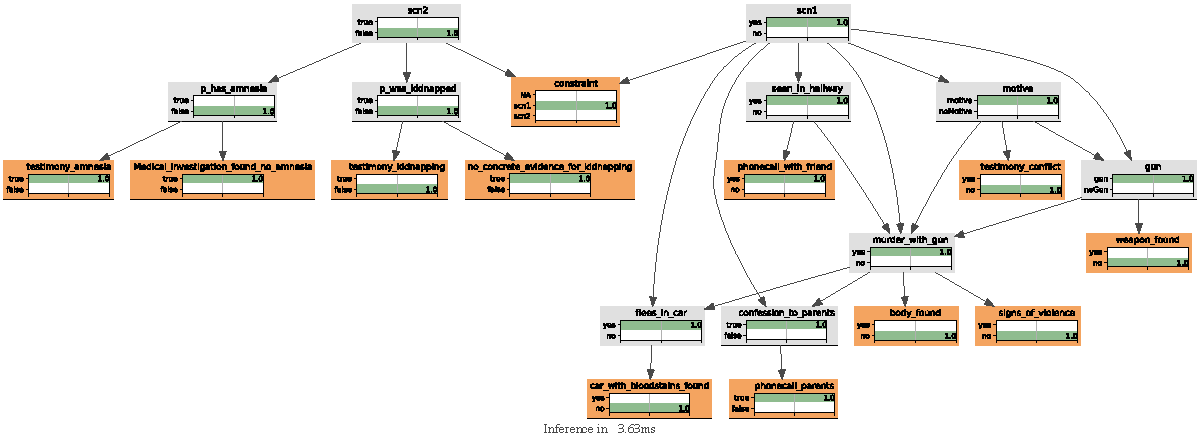
\includegraphics[width=\linewidth]{images/oldnetwork.pdf}
\caption{Example of subjective probability estimation resulting in a guilty verdict for insufficient evidence}
\label{love}
\end{figure}%


In general, it is hard for modellers to rationally consider all possible evidence states. This might lead to the bias demonstrated in the network. Though the network might respond well to situations where all evidence as presented in the trial is present. This brings up questions about the use of BNs in general: do we really need to consider these states where the evidence is different from the evidence as presented in the trial? Since specifying the joint probability distribution is necessary in BNs, we have to specify all of these numbers. Anyway, if we want to take BNs seriously, they need to be correct over all possible evidence states.

 The aim of this project is to define a method for the modeller to evaluate the BN over all possible evidence states, by grounding the BN in an agent-simulation of a crime. We can model crime cases using simulations to a level of realism we desire, measure the frequencies of events that emerge out of this simulation by running the simulation multiple times. In the agent-based system, we have full control over and full knowledge of the world that we are reasoning about, hence we can create a grounding that can be used to evaluate the BN. We can test whether our method of evaluating all possible evidence states works by comparing the predicted output of the BN with the frequency information about the output from the simulation. Then, we will discuss whether it is plausible that this method of evaluation generalises to real life\footnote{The simulation can be interacted with at \url{https://shielded-journey-34533.herokuapp.com} \\ Code for this project can be found at \url{https://github.com/aludi/simulationTest}}.

\newpage

\section{Background}

% reasoning with evidence
%Ook kort bespreken/benoemen: Di Bello and Verheij (2018) discuss how central analytic goals can be handled using each of the approaches.
We want to create grounded Bayesian Networks for reasoning with evidence. This can be done by creating a agent-based simulation, building BNs based on the events in this simulation, and testing the evaluation method on that BN. In this section, the relevant background is laid out on reasoning with evidence, Bayesian Networks, existing evaluation methods for BNs, and agent-based simulations.


\subsection{Reasoning with evidence}
We consider three main directions in the field of reasoning with evidence within law \citep{Verheij2015}, \citep{diBelloVerheij2018}. 

The first direction is via argumentation approaches, where hypotheses and evidence are represented as propositions that attack or support each other, as originating in \citep{wigmore1931} and in part unified by \citet{dung1995}, for a historical overview see \citep{benchcapon2019}. An example of argumentation research in AI and law is ASPIC+ \citep{prakkenEtal2013}. 

The second direction is via scenario approaches, where coherent hypotheses are combined into stories \citep{penningtonHastie1993}, \citep{wagenaar1993}, which are supported with evidence. Different types of stories need different pieces of evidence to be considered `valid' or `anchored' stories, and the extent to which different stories are anchored in the evidence determines how we assess them. 

The third direction is via probabilistic approaches, where hypotheses and evidence are assigned probabilities and the relation between hypothesis and evidence is represented with conditional probability, either by applying Bayes' law directly \citep{dahlman2020}, or by using Bayesian Networks. Bayesian Networks can represent aspects of a criminal case or can attempt a scenario-like hybrid and represent the entire case. Examples of this are: modelling actual crime cases \citep{kadaneSchum1996}, \citep{Fenton2019},  cases from fiction \citep{Fenton2012} or fictionalised crime cases \citep{vanLeeuwen2019}. The BN can also represent specific (forensic) aspects of a case, like DNA or blood-spatter evidence, for methods see \citep{Meester2021}. Bayesian Networks can also integrate aspects of argumentation \citep{wieten2019}, \citep{timmer2016}, or of scenario-based construction \citep{vlek2016}.



\subsection{Bayesian Networks}

A Bayesian Network (BN) is a directed acyclic graph that represents the joint probability distribution over a set of events \citep{pearl1988b}. BNs consists of nodes, arcs and conditional probability tables. A node is a random variable that represents an events. An arc represent a conditional relationships between two events, linking two nodes together. The two nodes are the parent and the child node, the probabilities in the child node are conditioned on the value that the parent node takes. The specification of these conditional probabilities is done in the conditional probability tables (CPT) of each node.


The combination of all nodes in the BN results in a full joint probability distribution over all nodes, which is 
\[P(x_1, ..., x_n)\]

We can decompose this using the product rule

\[P(x_1, ..., x_n) =  P(x_n|x_{n-1},... x_1) P(x_{n-1},...x_1)\]

Now, we see that $P(x_{n-1},...x_1)$ is also a joint distribution over all nodes, except node $x_n$. Hence, we apply the product rule again:

\[P(x_1, ..., x_n) =  P(x_n|x_{n-1},... x_1) P(x_{n-1}| x_{n-2}...x_1) P(x_{n-2},...x_1)\]

Keep applying this until we're at

\[P(x_1, ..., x_n) =  P(x_n|x_{n-1},... x_1) P(x_{n-1}| x_{n-2}...x_1) ... P(x_2 | x_1)P(x_1)\]

which is equivalent to 

\[P(x_1, ..., x_n) =  \prod_{i=1}^n P(x_i | x_{i-1},..., x_1)\]

In BNs, we know by definition that  

\[ P(x_i | x_{i-1},..., x_1) = P(x_i | parents(x_i))\]

Hence,

\[P(x_1, ..., x_n) =  \prod_{i=1}^n P(x_i | parents(x_i))\]

For every node $x$, hence, we will fill out the CPT

\[P(x_i | parents(x_i))\]




We show an example BN in Figure~\ref{exampleBN}. This is the basic form of the evidence idiom \citep{Fenton2012}: we have a cause as a parent node, and a consequence as a child node. In this context, we want to interpret the parent node as a `hypothesis', that we want to prove, but cannot observe directly. The child node is a piece of evidence that we can observe: it is either true, or false. Specifically instantiated, like in Figure~\ref{exampleBN}, we create a basic scenario: `suspect shot victim with gun' as the parent (hypothesis) node, and `bullet casings found on ground' as the child (evidence) node. We can use this network, with the probabilities as defined in the CPTs, to reason about the hypothesis given the evidence that we find.
 
In Figure~\ref{exampleBN}, the node `suspect shot victim with gun' is a hypothesis. Nodes with one or more incoming arcs are conditionally dependent on their parent node(s). In our example network, the node `bullet casings found on the ground' is conditionally dependent on its parent. The links between the nodes are links of conditional probability, and do not correspond to real-world causality, although they are sometimes interpreted as being causal \citep{Dawid2008}.

\begin{figure}[htbp]
\begin{center}
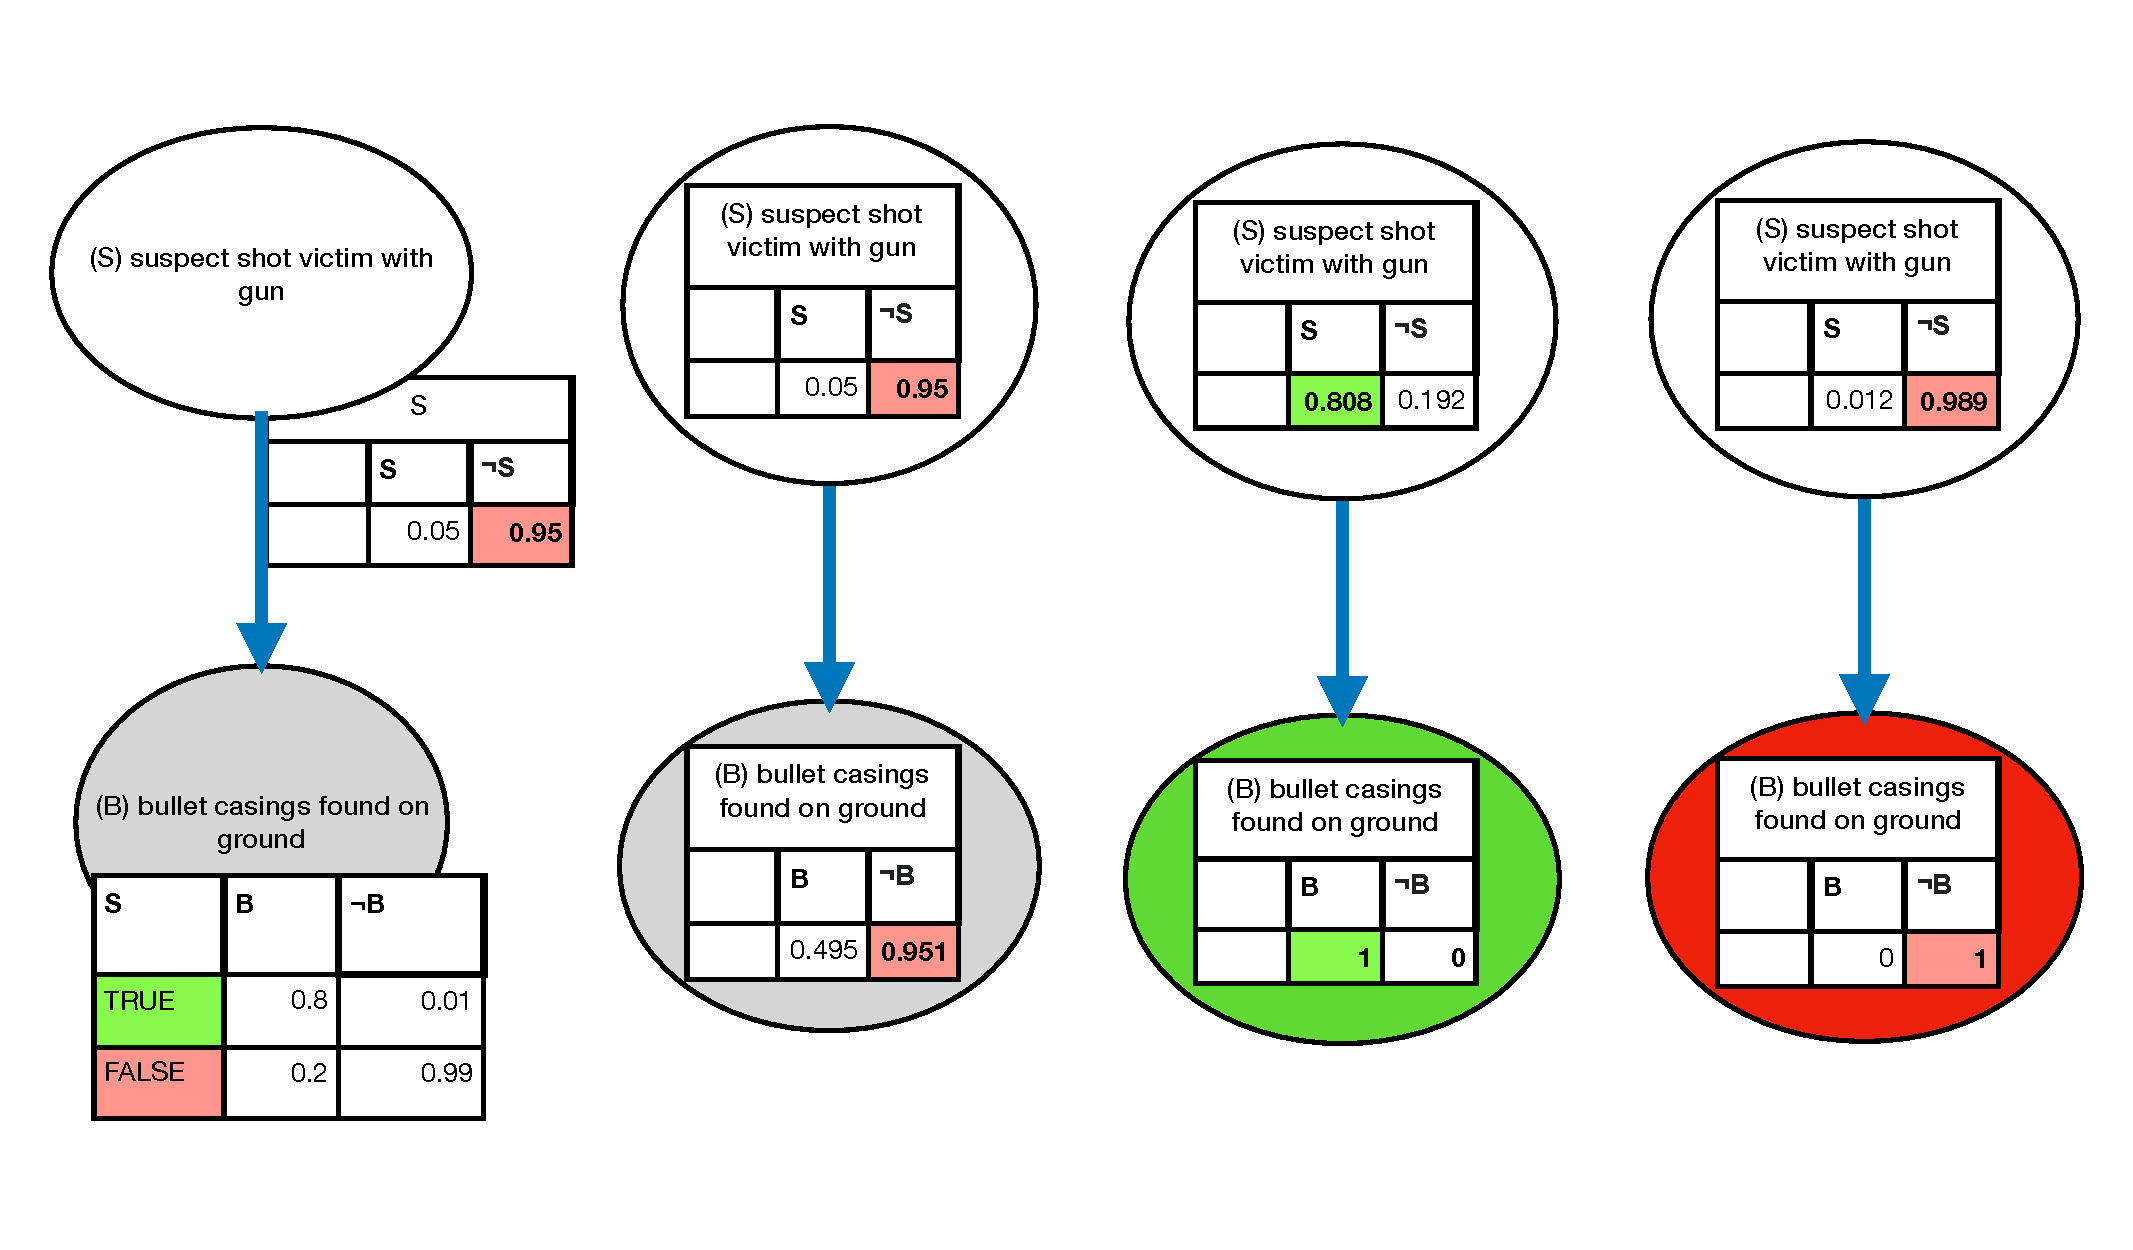
\includegraphics[width=\linewidth]{images/basicBayes}
\caption{Inference with Bayesian Networks: Defining the network with CPTS, entering no evidence, entering positive evidence, and entering negative evidence}
\label{exampleBN}
\end{center}
\end{figure}


The arcs and the CPTs tell us how we should reason about the hypothesis, given that we find some piece of evidence.


For a simple example, for a node with only one parent, we can just use Bayes law directly.


\[ P(H | E) =  \frac{P(E | H) \cdot P(H)}{P(E)}\]




To update to our network let us say that we found $B$, so there are bullet casings on the ground. We want to know what this new evidence will do to our belief in $S$. This means that we are updating our belief in $S$, or finding the posterior of $S$, based on the evidence that we found $B$.

\[ P(S | B) =  \frac{P(B | S) \cdot P(S)}{P(B)}\]
\[ P(B | S) = 0.8, P(S) = 0.05, P(B) = 0.8 \cdot 0.05 + 0.01 \cdot 0.95\]
\[ P(S | B) =  \frac{0.8 \cdot 0.05}{0.8 \cdot 0.05 + 0.01 \cdot 0.95} = 0.808\]

So now we have found the posterior of $S$, our belief in $S$ has increased from its prior probability of $0.05$, to its posterior probability of $0.808$, given evidence $B$. On the other hand, if we do not find bullet casings on the ground, our belief that the suspect shot the victim decreases from 00.5 to 0.012. 


Hence, we can exactly specify how our belief in a hypothetical event changes given all possible values of the evidence.This is the simplest form of Bayesian reasoning, with one piece of evidence, and one hypothesis. The general form of the update is more complicated (see ....).


In real-life situations, we are constantly reasoning with many pieces of evidence that might be conditioned on more than one parent node, resulting in tedious and error-prone calculations if we would do them manually. This is where Bayesian Networks are useful. 



We can outsource the Bayesian calculation to the BN, however, the network itself has to be constructed in some way. This can be done by hand by modellers, in (proprietary) software with a GUI like AgenaRisk or Hugin. They can also be built, by hand, or automatically constructed from datasets in PyAgrum, \citep{pyagrum2020}, a free Python software package. In this project, PyAgrum was used.



\subsubsection{Evaluating Bayesian Networks}

Bayesian Networks have been used to model reasoning with evidence in criminal cases, although these methods have not been used in court. However, even though there are methods for building BNs, it is unclear how we should validate and evaluate them. 

In data-rich domains, we can train Bayesian Networks on large amounts of frequency data and estimate the accuracy of the BN by cross-validation. We define a training set and a test set of the data (usually a 80/20 split). We construct the network based on the training data, 80\% of the input. Then, we test if the network learned the correct conditional probability relations on the final 20\% of the data, by comparing the expected output in the test data to the predicted output from the BN \citep{chen2012}. The 80/20 split allows us to measure to what extent the network is performing well on the entire dataset, and not just overfitting on the data that it has access to.

However, this approach towards BN validity through accuracy is implausible in BNs for court cases. The court cases involve one-of-a-kind events \citep{schum1982}, which means that it is unlikely that we can find frequency data on most of the nodes present in our BNs. This means that we cannot do an 80/20 type split in our data, as we only have one piece of data, which is the court case that we are modelling. This is why the probabilities in the BNs for court cases not pure frequencies, but instead subjective probabilities based on estimated frequencies, either elicited from experts or estimated by the modeller.

There are other ways of evaluating BNs than accuracy. The evaluation methods used by \citet{Fenton2019} and \citet{vlek2016}, who both model BNs based on real case studies, confine themselves to two approaches:

\begin{enumerate}

\item \textbf{Sensitivity analysis}

Sensitivity analysis tests the effect of small parameter changes in the CPTs of nodes on the outcome of the network. This is useful if the outcome of the network hinges on elicited or subjectively estimated probabilities. A sensitivity value of near 0 means that at the point of the CPT, a `small' change in the parameter would result in an infinitesimally small change in the output probability. That the CPT is not sensitive at all and a misestimation might not matter so much. However, a large sensitivity value means that the value is very sensitive to change : a small change in CPT might result in a meaningfully different output.  Since Bayesian Networks have many parameters per node, it is not trivial to perform a sensitivity analysis that takes into account all the nodes in the network, and interpret the results in a meaningful way - this would be an $n$-way sensitivity analysis \citep{gaag2007}.  

In \citet{vlek2016}, sensitivity analysis is mentioned, but not applied. On the other hand, in \citet{Fenton2019}, each individual hypothesis node is subjected to sensitivity analysis, to find out for how each of the parameters in the nodes need to change in order to result in a 0.95 or a 0.99 posterior for guilt. There are only a few ways that individual nodes can change that would result in a high probability of guilt, from which the authors interpret that the constructed BN is robust to small inaccuracies in subjectively elicited CPTs. However, in the paper, this is only shown for one evidence state. It is not clear how the BN would respond to `counterfactual' pieces of evidence.


\item \textbf{Cumulative evidence}

Another way of evaluating the response of the BN, is by seeing its response to cumulatively setting evidence. This way, we can see how much each piece of evidence (from the defence or the prosecution) changes our belief in the posterior of the output node(s). We could subjectively assess if it makes sense that a certain piece of evidence has a large, or small, effect on the posterior. In both \citep{Fenton2019} and \citep{vlek2016} this cumulative approach shows that, in general, the evidence from the defence decreases our belief that the suspect is guilty, and evidence from the prosecution increases our belief that the suspect is guilty. However, in both cases, the BN is only evaluated on one state of evidence. Both cases only test the cumulative probability of the output node by turning the evidence nodes to values that correspond to the findings of the court. However, this is a risky move, since this might lead to overfitting the probabilities in the CPTs, so that the network seems to reflect the right `evidence strength' on the court-found state of evidence, but is actually misrepresenting other combinations of evidence, without a way of checking if this is the case.




\end{enumerate}


Our findings in Figure~\ref{love} show that it is necessary to consider all possible combinations of evidence. If we have tunnel vision and only focus on the state of evidence that is found in court, we might create a network that overfits on one state of evidence. This means that if there was a re-trial and the court would decide that some pieces of evidence are not admissible after all, the BNs might show the unreasonable behaviour. Additionally, if we are building the BN before or during the court case, we cannot know yet which state we are in, as none of the evidence has been established yet. Therefore, the network should work correctly over all possible evidence states. If we want to take the premise behind BNs seriously, we have to create a network that gives sensible results for all possible combinations of evidence, not just the valuation of the evidence that is initially established in court.

\subsection{Simulation}

We are using agent-based simulations to investigate methods for evaluating Bayesian Networks. Agent-based modelling is a modelling primitive that allows researchers to study models in which agents interact with their environment and with other agents \citep{gilbert2000}. 

Agent-based modelling is useful for simulating criminal behaviour in spatially explicit ways. The actions of a thief and victim are constrained by geography and local knowledge. For instance, a thief cannot move through buildings like a ghost, or steal from someone they have not seen. Due to specific interactions that arise out of the circumstances in each run of the simulation, we can collect frequency information about all the relevant events in our modelled scenario that would be hard to estimate with subjective probabilities or with mathematical (non-spatially explicit) models. Since we have full knowledge of the frequency of events in the simulation, we can use it as a `grounding', or baseline. In a sense, the simulation is a data-generating environment for criminal cases. If we look at the taxonomy of agent-based model levels in \citep{gilbert2005}, where level 3 is a simulation that really reflects the real world, and level 0 is a `caricature of reality, as established with simple graphical devices', the simulation in this paper is at level 0, to reduce unnecessary modelling and time complexity. In this project, the simulations are programmed in Python using the MESA framework  \citep{mesa2020}.

\newpage

\section{Method}

Our goal is to establish a method for evaluating BNs by preventing overfitting on one evidence state. We can consider an approach in four stages.

\begin{enumerate}
\item \emph{Scenarios} We need a set of alternative scenarios that are to be modelled. These scenarios are written description of crime scenarios that contain the hypothetical events and evidence for these events, as postulated by the prosecution and defence. 

\item  \emph{Simulation} Based on this written description of the scenario(s) to be modelled, an agent-based simulation is created, by first identifying and operationalising all relevant agents, objects and environments, and secondly identifying and operationalising all relevant events. Depending on the goal and complexity of the scenarios to be modelled, the granularity and overall level of the simulation should be considered. The simulation should be repeated until we find the limiting frequency of all events. These frequencies are collected.

\item  \emph{Construction} The collected frequencies are used by the K2 algorithm to automatically build a Bayesian Network of the simulation. 

\item  \emph{Evaluation} The generated Bayesian Network is evaluated on all possible states of the evidence.

\end{enumerate}

\subsection{Scenarios}
We start our process with one or more written scenarios. These scenarios can be obtained from abridged or simplified court case descriptions of the crime, or they can be wholly fictional (such as in this paper). The scenarios should contain all and only those hypotheses and evidence that are relevant to the case. Both the prosecution and the defence should be able to select relevant events and their evidence. 

\subsection{Simulation}
We can think of the simulation as having two parts: a model of reality, and a way of observing the model by observing variables that the modellers deem interesting. In this paper, the model of reality is an agent-based simulation, and the observation procedure are random variables (or, reporters), which become nodes in the BN.

The agent-based simulation is a simulation that should include the possibilities for all the scenarios as outlined in step 1. It should contain agents, objects and an environment. The level of detail or real-world validation at which agents, objects and environments are modelled depend on the purposes of the environment.


In the simulation, certain events can be brought about. Any one of the above-mentioned events can happen. We need a way to observe these states: this is where reporters come in. A reporter is a random variable that is reports the outcome of a relevant event in the simulation and is embedded in the code. If an event happens (or does not happen), the reporter reports that the event is true (or false). In essence, the reporter ($R$) is a random variable (RV). In short, a random variable is a function that maps an event ($e$) to a truth value:

\[ R : e \rightarrow \{0, 1\} \]
No matter how many reporters we define, we can combine all reporters at the end of one run of the simulation into a global state $G$.

\[ G = (e_0 \rightarrow \{0, 1\} \times e_1 \rightarrow \{0, 1\} \times ... \times e_n \rightarrow \{0, 1\})\]
 or, for $n$ reporters:
 
\[ G = R_1 \times R_2 \times... \times R_n\]

We collect these global states over the number of runs that we do for each experiment, which results in the output $O$ of this stage of the method, is a series of global states, one for each run:

\[ O = (G_0, G_1, ... G_{runs})\]


\subsection{Construction}
The output of this method is the collection of runs $O$, where each run is the global state $G$ of the simulation, as measured by the random variables $R$. These random variables become the nodes in the Bayesian Network.

The Bayesian Network is generated automatically, using the automated BN learner method as implemented in pyAgrum. There are several learners implemented in pyAgrum.\footnote{An introduction to structure learning using PyAgrum: \url{http://webia.lip6.fr/~phw/aGrUM/docs/last/notebooks/structuralLearning.ipynb.html}} The algorithm used in this experiment to structure the Bayesian Network from the simulation data is the K2 algorithm \citep{Cooper1992}. 

The K2 algorithm is a greedy search algorithm that attempts to maximise the posterior probability of the network by correctly connecting parent nodes to child nodes. It takes an ordering on the nodes as input. The first node in the ordering $X_0$ does not have any parents. For two nodes $X_i$ and $X_j$, $X_j$ cannot be the parent node of $X_i$ if $j > i$: a node can only have a parent that is earlier in the ordering. The algorithm processes each node $X_i$ by adding possible parent nodes to $X_i$ (as constrained by the ordering), and maximising the score of the network. The algorithm stops if there are no parents to add, no parents improve the score, or the node has reached the maximal number of parents \citep{Chen2008}.

Due to this ordering constraint, the K2 algorithm is efficient. However, finding the ordering of the nodes as input for the network is not trivial. The ordering should be meaningful, to reflect causal or temporal information present in the domain. By adding the nodes to the simulation in the relevant order, we can ensure that the order is temporal. 



\subsection{Evaluation}

We can evaluate the response of the Bayesian Network using the effect of cumulative evidence on the posterior probability of the output nodes. This means that we order the evidence nodes chronologically, then instantiate every evidence node to a truth value (either T or F) in order. Then, we measure the posterior probability of all output nodes. This results in a diagram or table where we can see the evidence strength of each piece of true or false evidence reflected. We propose a method for evaluating Bayesian Networks over all possible global evidence states in this paper. This method is described here.

\begin{enumerate}
\item Select all evidence nodes (a total of $e$ states).
\item Order the evidence nodes chronologically.
\item Select all possible evidence states. An evidence state is a valuation of evidence, where for every evidence node, a truth value is specified. For this simulation, an evidence state could look like (1, 0, 0, 1), which would correspond to finding that the psychological report is true, the agent was seen on camera, but not seen stealing, and the object was lost.

If there is enough data available, as is the case in our simulation, we can extract all possible evidence states automatically. If we do not have enough data, we need to manually consider each evidence state (start with $2^e$ states, ask an elicitor to delete states that are not possible).
\item Create a baseline. For each possible evidence state, create a total probability distribution over all possible output states. Speaking generically about two alternative, non-mutually exclusive outcomes scenario 1 (scn1) and scenario 2 (scn2), we need to find a probability distribution over $scn1, \neg scn1 \land scn2, \neg scn1 \land \neg scn2$ that is constrained by $P(scn1) + P(\neg scn1 \land scn2) + P(\neg scn1 \land \neg scn2) = 1$. Or, a weaker version, we create a preference ordering on $scn1, \neg scn1 \land scn2, \neg scn1 \land \neg scn2$, without specifying probabilities. 

In our simulation, or in data-rich environments, we can automatically create this total probability distribution, since we can count the conditional frequencies that occur in simulation. In real life, a preference ordering or probability distribution over the possible outcomes would need to be elicited by modellers from experts.

\item For every possible evidence state, turn the relevant nodes in the BN on in order. At each step, record the posterior probability over the output nodes. Automatically convert the probability distribution over the outcomes into a preference ordering.
\item Compare the BN prediction of output nodes given evidence to the prediction establishes in step 4). Once all evidence is added, we can calculate the divergence of the BN prediction and the actual frequency in the simulation by \[|P(output|E) - F(output|E)|\], where $E$ is the total set of evidence in a given state.
\item Calculate the total accuracy per output node by \[\frac{\sum_{i=0}^{e}|P(output | E_i) - F(output| E_i)|}{e}\] For the preference ordering, we do the same, only we calculate a counting score: when the preference ordering extracted from the BN is the same as the one from the simulation, we give a point, otherwise we do not, then average this over all sets of evidence.
\end{enumerate}


\newpage


\section{Case Study: Robbery at Grote Markt}
We illustrate the method by means of applying it to a case study of a robbery at the Grote Markt, the central square in Groningen.

\subsection{Experimental Set-up}
BNs were created and evaluated based on different number of runs, to evaluate how the accuracy of the BN depends on the data available to it. 

We want to create both a ground truth, that are the frequencies that we're interested in, and then the probabilities that are going to approximate it so that we can check the accuracy of the network. To find the ground truth, we need to find the limiting frequencies of the events in the simulation, the simulation was run 10,000 times. One thing we want to find out is the necessity of precision on the outcome of the networks. This was done by changing the number of runs that the BN was created on. The different number of runs of the simulation were [1, 5, 10, 20, 40, 60, 100, 200, 500, 1000~] for creating the BNs.


Every simulation was run for 100 steps, or until both agents were in their target states. 


\subsection{Scenarios}


We have established three different scenarios. In all scenarios, there are two people walking around the Grote Markt. One person is young, and the other person is old and carries a valuable object. 

In scenario 1 (scn1), the young person sees the old person, assesses whether the object is valuable enough to risk stealing, and if the old person is vulnerable enough to steal from, and a motive is established. Then, if the young person has a motive, they will attempt to sneak up on the old person. When they get near, they steal from the old person.

In scenario 2 (scn2), the young person might still be doing all of the above (or they might not), however, before they can steal, or if they decide that they're not stealing at all, the old person drops the object accidentally.

In scenario 3, neither scenario 1 or scenario 2 happens. The people walk around at Grote Markt and then go home. We do not have to represent scenario 3 explicitly, it can be represented as neither scn1 nor scn2.

For our evidence, we have a psychological assessment of the young person, that assesses whether they are psychologically capable of stealing from the old person. We also have cameras at Grote Markt that show whether the young person was seen at all, or was seen stealing. Additionally, we have the fact that the object is gone or not.


%In our simulation, there are two agents walking around the area of Grote Markt. One of the agents is old and carries a valuable object. The other agent is young, and might potentially steal the object. There are three things that can happen in this simulation: nothing is stolen or lost, the object is lost accidentally by the old agent, or the object is stolen from the old agent by the potential thief. If the potential thief sees the potential victim, it decides whether the object is worth the risk of stealing, and if the potential victim is vulnerable enough to steal from. If both of these conditions are fulfilled, the agent becomes a potential thief, and now has a motive to steal from the old agent. The agent will attempt to sneak up on the victim, and steal the object from the old agent. At some point, the old agent realises that their valuable object is gone. As evidence, we have a psychological report that estimates whether the young agent is capable of the crime, we might have video footage of the thief stealing the object, and we have the fact that the potential thief shows up on camera. 

%Additionally, outside the described scenario, we also have access to the `mental' state of the potential thief, so we know whether they actually consider the old agent vulnerable, and whether they find the object itself valuable. We also know if the thief is actually intending to sneak up on the other agent.


\subsection{Simulation}		% REPLICABILITY

Now we need a way to transform the natural language descriptions of the events in the scenarios to observable events in the simulation. First, we identify all relevant actors, objects and environments in the scenario and operationalise them in a simulation. Second, we identify the relevant reporters. 



\subsubsection{Agents} 


Agents can interact with other agents and with their environment. Every agent has features, functions and roles associated with them. The agents in this simulation are created from the MESA agent class. These are goal-based agents.
Based on the scenarios as described in the previous step, we want to create one older, vulnerable agent, and one younger potential thief. In principle, the simulation is flexible enough that any agent can be a thief, as motive is determined by a risk-trade-off and not something inherent to the agents themselves. However, since we wanted to avoid problems with identity and follow the scenarios, we made sure that only one agent would be the thief, by having it have an object that was not valuable and an age that was not vulnerable. The behaviour of the agents is depicted in Figure~\ref{behaviourGM}.



All agents have the following \textbf{attributes}:
\begin{description}
\item [role] Every agent has a role of either victim or thief. In a more realistic scenario this role would be assigned based on behaviour, but in this simulation, this was done at the start (because the scenario allows for one thief, and one victim). However, the role `thief' does not mean that the agent will actually steal, and the role `victim' does not mean that the agent will be robbed\footnote{From now on the `' around the roles are dropped}: if the victim drops the object, or if the thief and victim never meet, these roles are not fulfilled by the agents. Hence, the role only implies a certain potentiality.
\item [id] Every agent has an ID. The thief has ID 1, the victim has ID 0.
\item [object] The thief has an object with a value of 0, the victim's object has a value drawn from a uniform distribution between 500 and 1000. 
\item [goal location] The goal location of the agent is either it's initial goal location that was assigned at the start, or, when the agent has a motive, it is the current location of the victim agent. The initial goal location for each agent is drawn randomly from any of the accessible locations at the edge of the map.
\item [age] The thief's age was 25, the victimt's age was drawn from a uniform distribution between 60 and 90.
\item [risk threshold] The risk threshold for the victim agent was set to 5000, such that it is never worth for it to steal, the risk threshold for the thief is randomly drawn from a uniform distribution between 800 and 1200.
\item [age threshold] The age threshold signifies at what age an agent considers another agent vulnerable: older agents are more vulnerable than younger agents. The victim's age threshold is set to 100, it will only steal from agents that are 100 years or older. The thief's threshold is randomly drawn from a uniform distribution between 50 and 100.
\item [steal state] The possible steal states are: MOTIVE, SNEAK, STEALING, SUCCESS, N, DONE, LOSER.
\end{description}

All agents have the following \textbf{actions}:

\begin{description}
\item [hang around] Agents move around randomly.
\item [walk] Using standard mesa functionality, at every step of the agent, the agent moves 1 cell in the Moore neighborhood. The agent attempts to walk towards its goal state, whether that is a moving agent or their goal state. They move towards their goal state by taking the possible step that minimises the distance between their goal and themselves using the Euclidian distance as measure (this does not take buildings into account).
\item [escape]  Given the use of Euclidian distance instead of a smarter, geographically-informed approach (using waypoints or something similar), agents can get trapped in tight corners of the simulation when they're moving towards their goal. There is an epoch tracker that counts `stuckness' and then moves the agent into the `hang around' state, of random movement, for a given time. This means eventually the agent will randomly move away from the `stuckness'.
\item [see] every agent has a visual range of 10 cells. This means that all simulation objects (agents, objects) within that radius are selected. Actual vision is only calculated based on line-of-sight, which means that for each object in range, we use the Bresenham's line algorithm to select the relevant cell that lie on the `environment grid' in between the agent and the object that it is seeing. For every cell on the straight path between the two objects, we check whether it is `accessible' or `non-accessible'. Agents, and light, cannot pass through `non-accessible' cells. This is an abstraction, in real life there are windows. So if there's one `inaccessible' cell on the list of cells that are the straight line between seeing agent and object, the agent is not able to see the object. 
\item [decide valuable] Once the thief has a targeted victim, the thief knows the value of the object of the victim. In this function, the agent decides whether the object is worth stealing. If the value of the object is larger than the risk threshold of the agent, the object is deemed valuable.
\item [decide vulnerable] Once the thief has a targeted victim, the thief knows the age of the victim. In this function, the agent decides whether the victim is vulnerable enough to steal from: if the age of the victim is older than the age threshold, the thief considers the victim vulnerable.
\item [sneak] Agent moves to the position of the victim, only it can move with a radius of 2 (hence, at higher speed).
\item [steal] Whenever the thief is in the same cell as the victim - and they're both still within the simulation (so the victim has not reached its goal yet), the thief steals successfully.
\end{description}






\subsubsection{Environment}

The environment is a discrete grid of size $x=75$, $y = 50$ that represents the geography of the Grote Markt. The real area of interest is approximately 425m x 280m, as estimated by the distance tool on Google Maps. This means that one cell in the simulation is equivalent to a square of 5.6m x 5.6m in real life. An agent can move 1 cell per time-step, which means that, given an average human walking speed of 1.4m/s \footnote{\url{https://en.wikipedia.org/wiki/Preferred_walking_speed}}, one time-step is equivalent to 4 seconds in real life. For the purposes of this simulation, this spatial and time resolution is high enough.

To simulate which parts of the Grote Markt were accessible to the agents, we had to convert a map image of the Grote Markt into an agent-readable world. This was done by writing a method to convert screenshots of maps into an agent-readable environment. The map was screenshotted from \url{http://maps.stamen.com/terrain/#18/53.21618/6.57225} and converted into greyscale. A grid was overlaid on the image. On the greyscale map, the color of the buildings was in the range of (189, 199): cells within this range were coded as `inaccessible', since agents cannot walk through buildings. All other cells were `accessible'. This resulted in a map shared by all agents that constrained their movements. The map constrains both vision and movement of the agent: we used this map to calculate the sight lines of both cameras and agents. An agent or a camera can only see another agent if there are no `inaccessible' grid cell on the sight line between the two, and the other agent is within their visual range. The environment is shown in Figure~\ref{groteMarkt}.
 
 \subsubsection{Objects} 
 There are two types of objects in the simulations, which are the valuable object, and the cameras. 

 In the scenario, an object is described as being in the possession of agents, or lost accidentally. In this simulation, the object was operationalized as being a feature of the agent, and not as an individual thing by itself.
 
 There are 5 cameras in the simulation. They are placed randomly on the `accessible' cells on the map. Every camera has a visual radius of 5, corresponding to a range of 28m, which is about equivalent to the visual range of real-life security cameras~\footnote{\url{https://securitycamcenter.com/how-far-can-security-cameras-see/}}.
 


%\item \textbf{We select all relevant events from the written description and attempt to operationalise them in the simulation.}
\subsubsection{Reporters}
We divide all all events into three classes: either an event is `evidence' (E), a `hypothesis' (H), or an ultimate `outcome' (O). 

The process of operationalisation is very subjective and depends entirely on the modeller's assumptions and their time, knowledge or skill constraints. The behaviour of agents, as reflections of actual people, can be modelled in a way that reflect real sociological theories of behaviour (such as in \citet{Gerritsen2015}), or with simple behavioural rules and a random number generator (such as here). The environment of the simulation can reflect a real-world geography with different affordances, or can be simplified. 

The operationalisation of the random variables is described below. 
\begin{description}
\item[(H) motive\_1\_0 ] agent 1's steal state is MOTIVE.
\item[(H) sneak\_1\_0 ] agent 1's steal state is SNEAK.
\item[(O) stealing\_1\_0 ] agent 1's steal state is STEALING.
\item[(O) object\_dropped\_accidentally\_0 ] At every epoch, there is a 1/500 probability that the victim agent will drop the object by accident. If the object is dropped, this reporter is turned on.
\item[(E) E\_camera\_1 ] agent 1 is seen on any one of the cameras.
\item[(E) E\_psych\_report\_1\_0 ] if the thief has a motive, we draw an estimated risk threshold and an estimated age threshold from two normal distributions (mean = victim age, sd = 20), (mean = value good, sd = 100). If the victim is older than the thief's minimal age threshold, and the object more valuable, we estimate that the psych profile states that the victim fits the thief's profile, else not. This is not represented spatially in the simulation itself.
\item[(E) E\_camera\_1 ] agent 1 is seen on any one of the cameras.
\item[(E) E\_camera\_seen\_stealing\_1\_0 ]  if any camera sees agent 1 when agent 1's steal state is STEALING.
\item[(E) E\_object\_gone\_0 ] if the object is dropped accidentally, or if the object has been stolen.
\end{description}



A global state where the thief stole the object and all the evidence pointed in this direction, would be represented as (reporters in the same order as in the listing above):
 \[1,1,1,0,1,1,1,1,1\]



\begin{figure}[htbp]
\centering
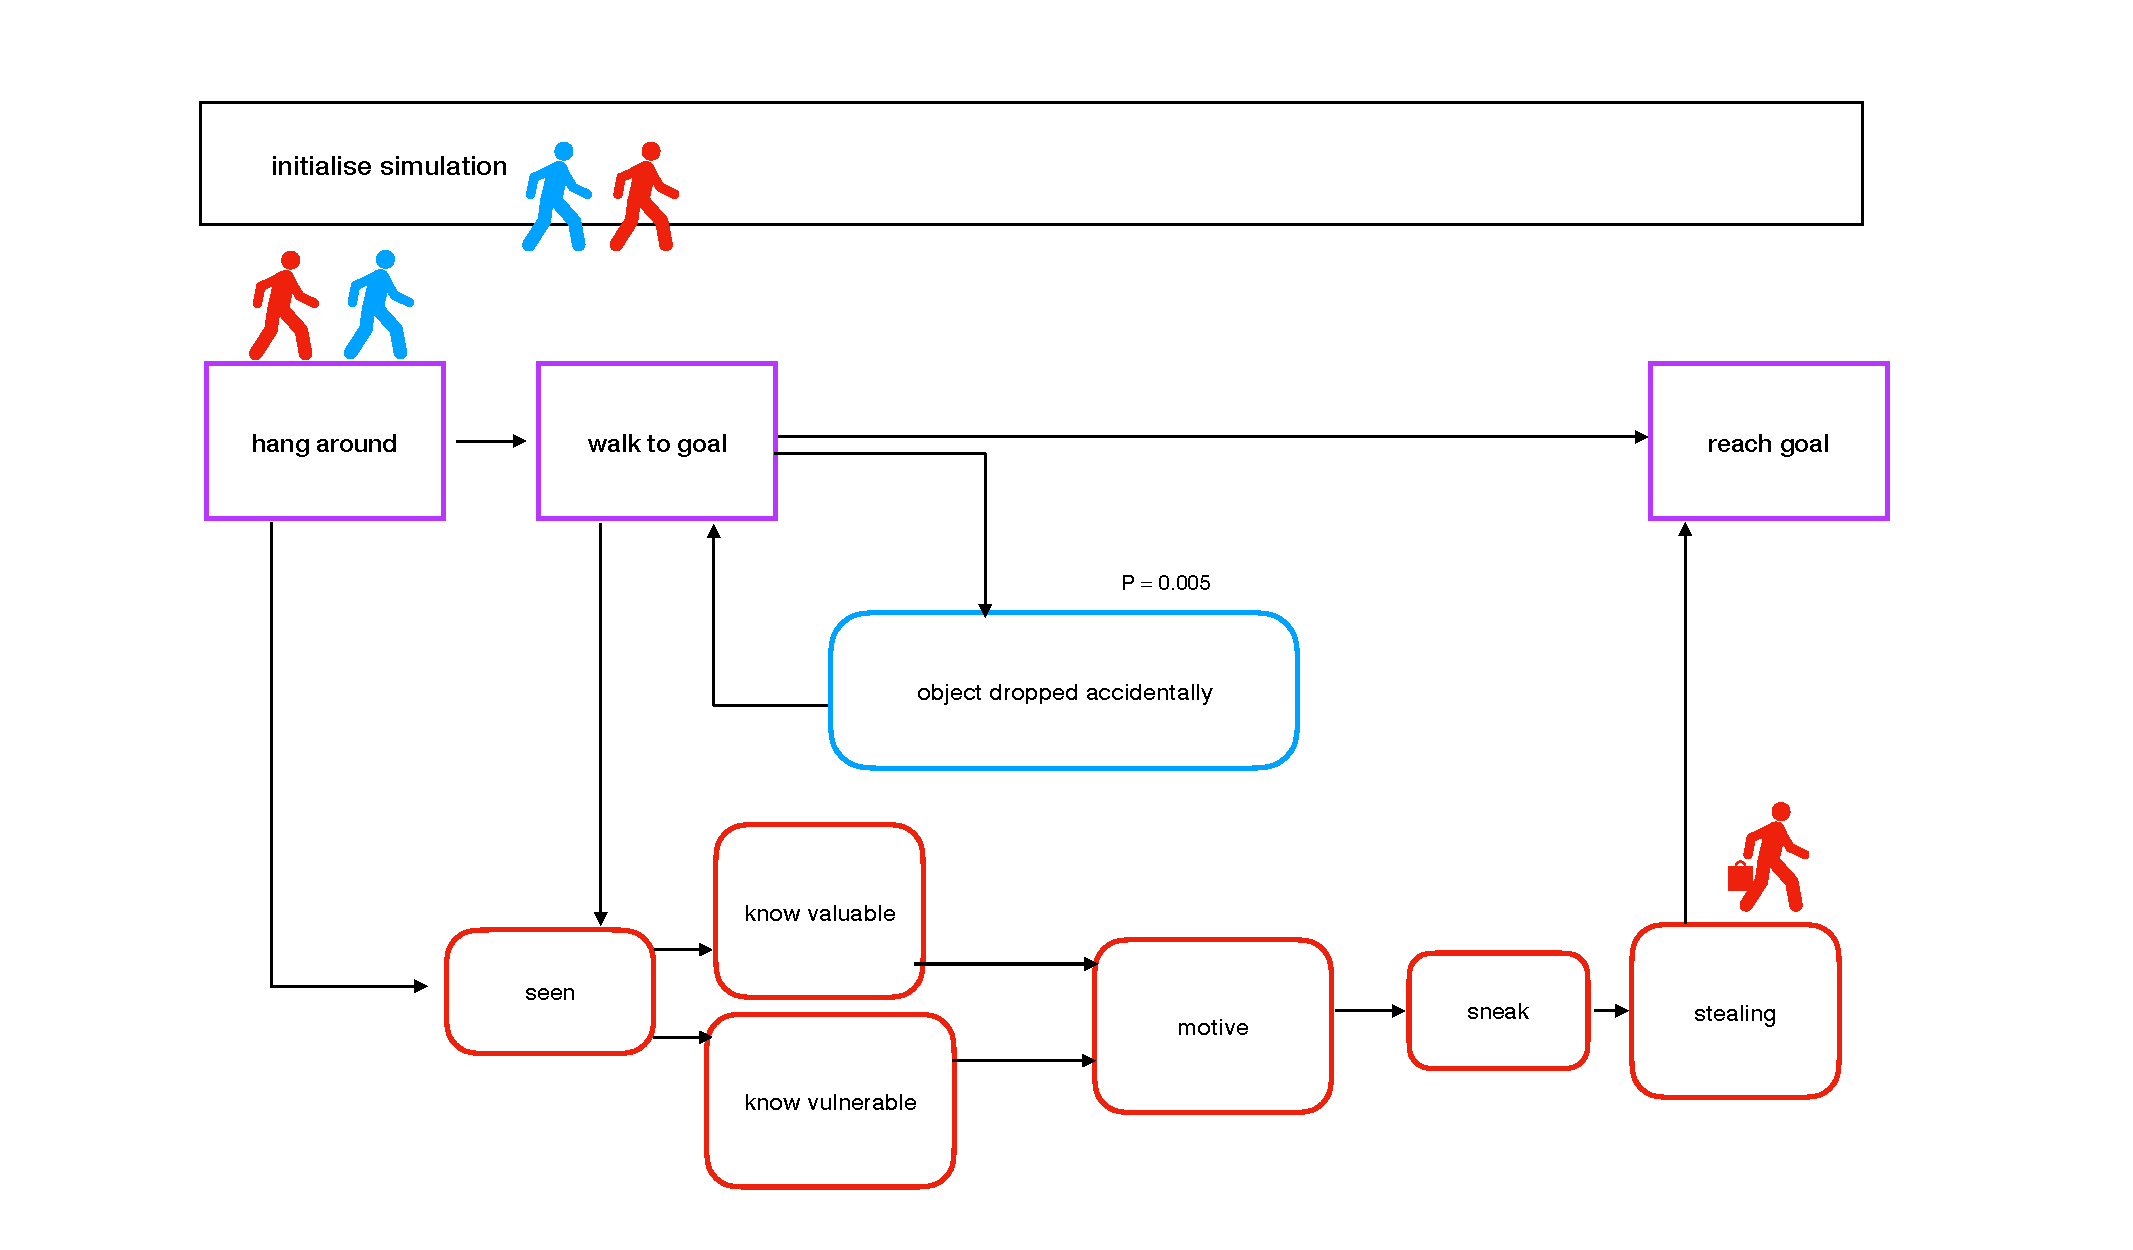
\includegraphics[width=\linewidth]{images/grotemarkt.pdf}
\caption{The behaviour of the agents. The nodes with rounded edges correspond to the nodes in the Bayesian Network.}
\label{behaviourGM}
\end{figure}

\begin{figure}[htbp]
\centering
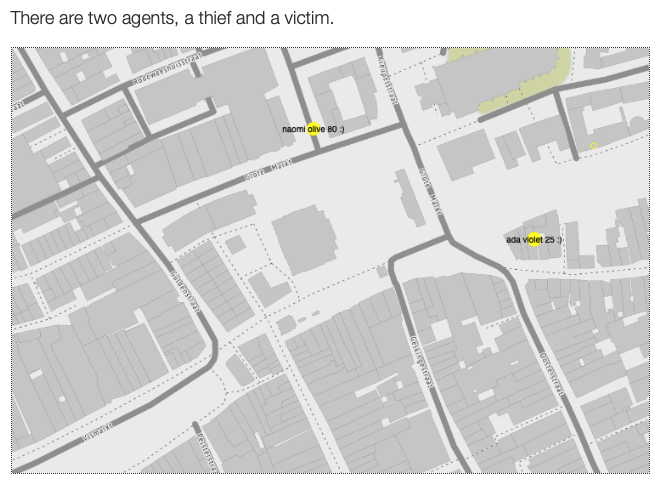
\includegraphics[width=0.75\linewidth]{images/grotemarktmap.png}
\caption{map of environment - 2 agents}
\label{groteMarkt1}
\end{figure}

\begin{figure}[htbp]
\centering
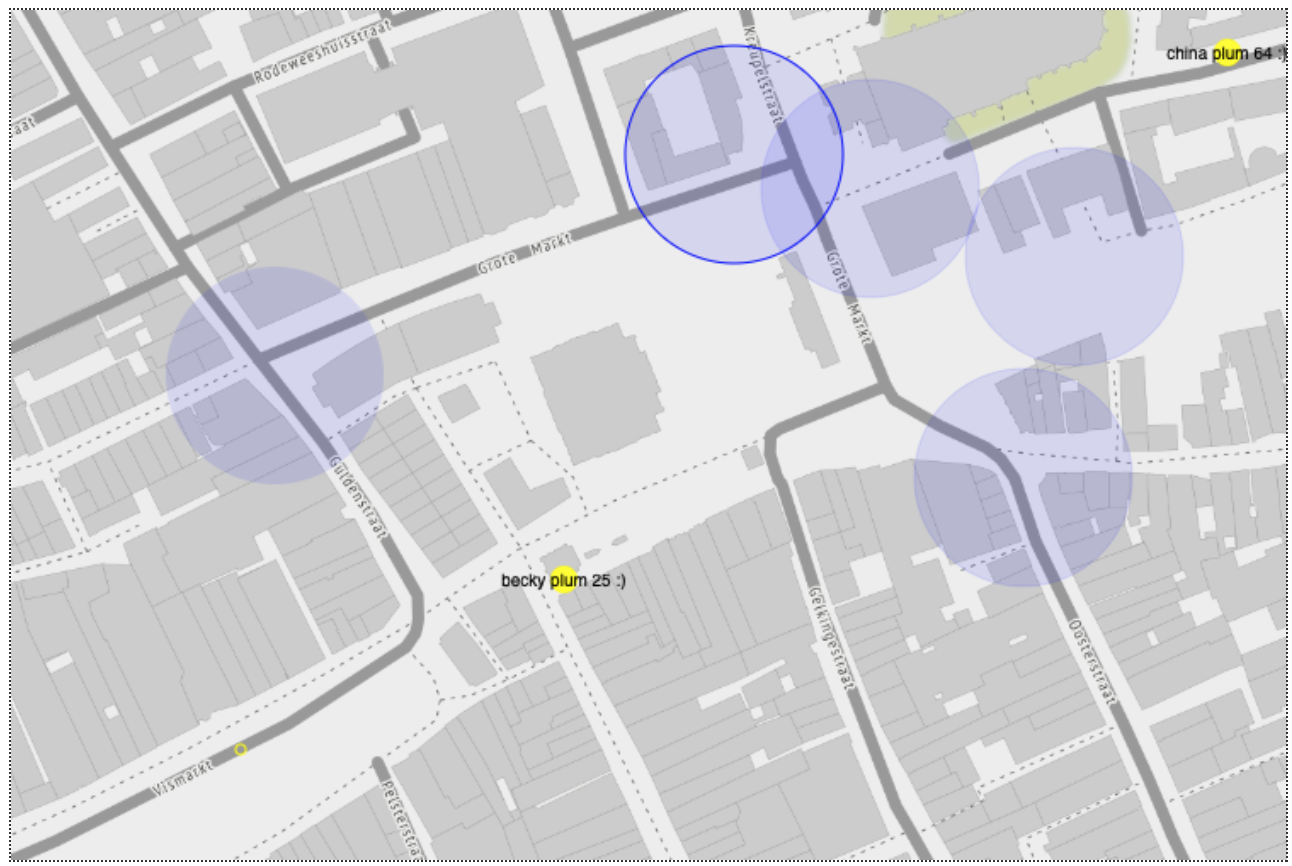
\includegraphics[width=0.75\linewidth]{images/agentGM.png}
\caption{Camera locations are randomly initialized}
\label{groteMarkt}
\end{figure}


\subsection{Construction}
K2 algorithm,  all are binary random variables. Ordering here.



\subsection{Evaluation}
Automatically done in code

Reasoning using LazyPropagation (exact inference) in Pyagrum.




\newpage

\section{Results}



We have a final Bayesian Network (Figure~\ref{bullet}), that was created from the K2 algorithm that contains all the nodes specified. The arcs between nodes are not causal but conditional. 

We have passed the structure of the network to the K2 algorithm (not automatically). 


We have a plot of the overall accuracy over all evidence sets of the network for both the `stealing\_1\_0' node and the `object\_dropped\_accidentally\_0' node (Figure~\ref{girl}). For a low number of runs, the network could not be created, hence the accuracy of 0. At around 10 runs, a network could be created, with an accuracy on all cumulative evidence states of around 0.75 for both nodes. Increasing the number of runs, hence, the data available to K2 to create the network, results in a higher accuracy. We have a frequency distribution over the possible states (Figure~\ref{fifteen}), where we see that most possible states occur infrequently, while one possible state [0, 1, 0, 0] occurs 70\% of the time. 

In Figures~\ref{nobody}, ~\ref{whirl}, we show cumulative evidence plots on both output nodes for two sets of evidence, on both a BN that was created from 10 runs, and on a BN that was created from 1000 runs of the simulation. Every plot shows the BN predicted output (bar on the left side), next to the actual frequencies in the simulation (bar on the right side).

In Tables~\ref{journal}, \ref{somebody}, we show the final cumulative probability and preference ordering for the output nodes as the worst (10 runs) and best (1000 runs) BN predicted them. In Table~\ref{heretic}, we show the frequency of the output for each possible evidence state, as well as the preference ordering, for the ground truth as found in the simulation.

\begin{figure}[htbp]
\begin{center}
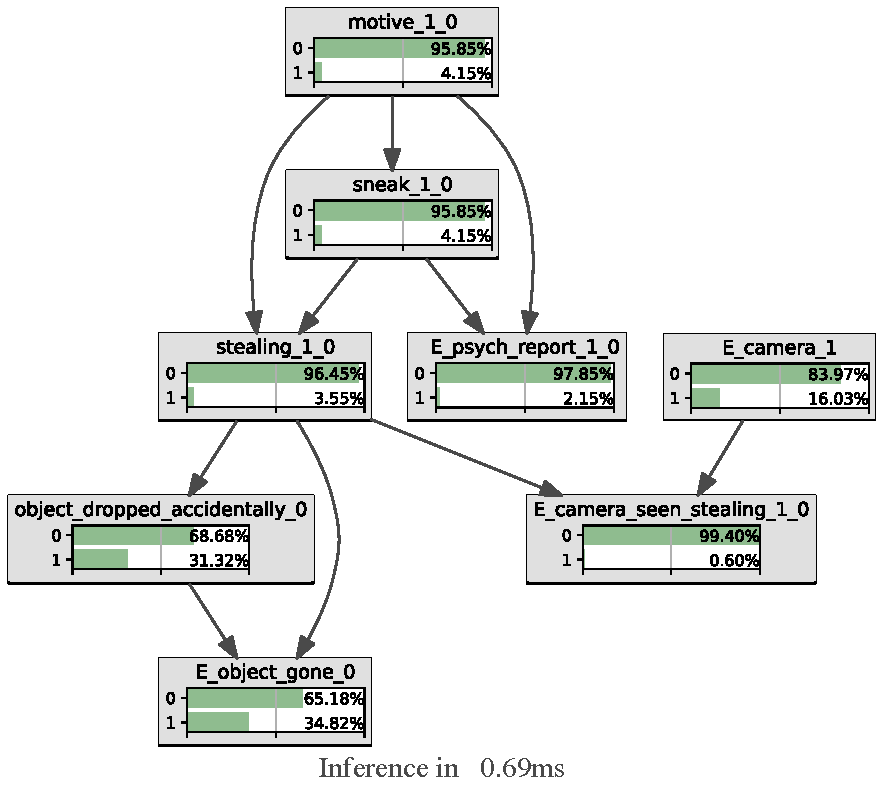
\includegraphics[width=\linewidth]{GroteMarktPrivateEND/bnImage/BNIMAGEGroteMarktPrivate.pdf}
\caption{The final network (1000 runs)}
\label{bullet}
\end{center}
\end{figure}

\begin{figure}[htbp]
\begin{center}
\begin{subfigure}{0.6\textwidth}

\includegraphics[width=\linewidth]{GroteMarktPrivateEND/plots/accuracy.pdf}
\caption{Accuracy of network based on the number of training runs}
\label{girl}
\end{subfigure}%
\begin{subfigure}{0.6\textwidth}
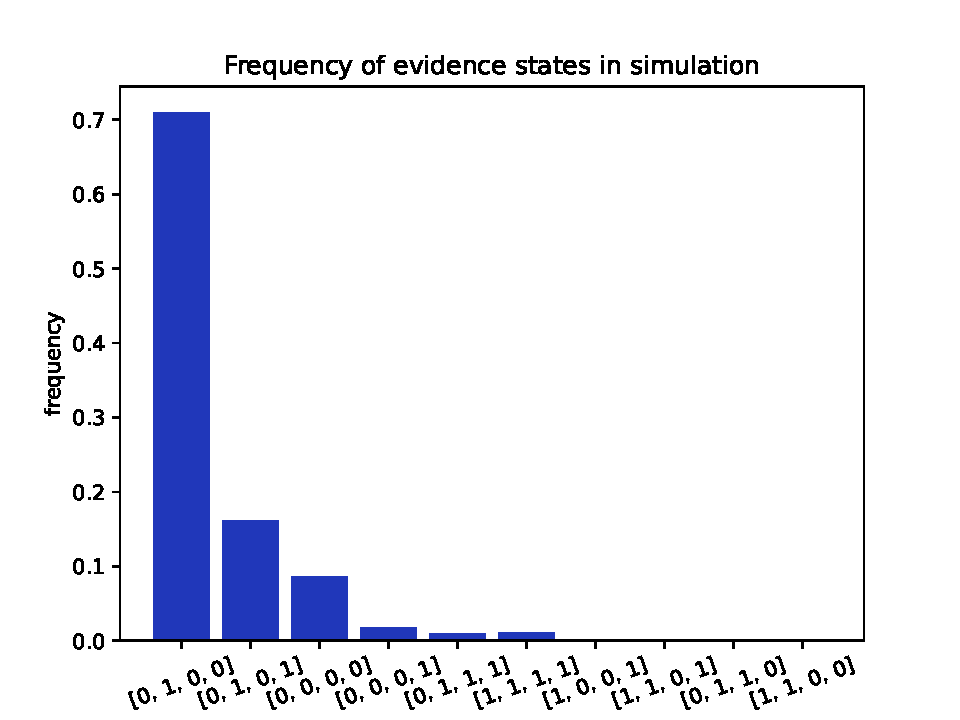
\includegraphics[width=\linewidth]{GroteMarktPrivateEND/plots/freqStates.pdf}
\caption{Frequency of states}
\label{fifteen}
\end{subfigure}
\end{center}
\end{figure}


\begin{figure}[htbp]
\begin{center}
\begin{subfigure}{\textwidth}
\makebox[\textwidth][c]{
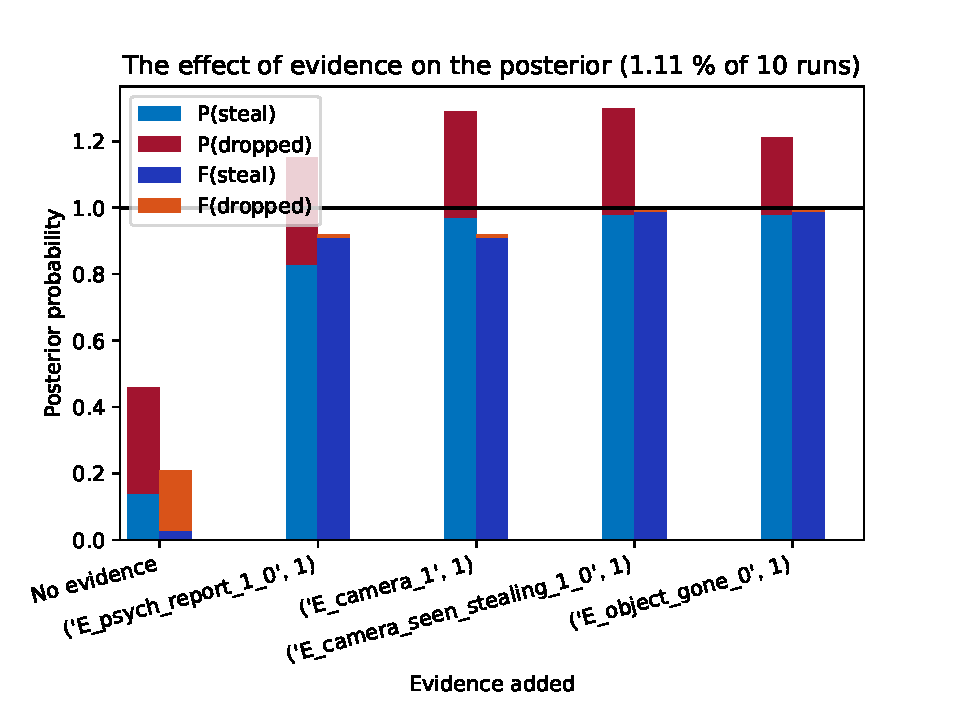
\includegraphics[width=0.7\textwidth]{GroteMarktPrivateEND/plots/freq/evidence_progress_GroteMarktPrivate_10_1.1100.pdf}
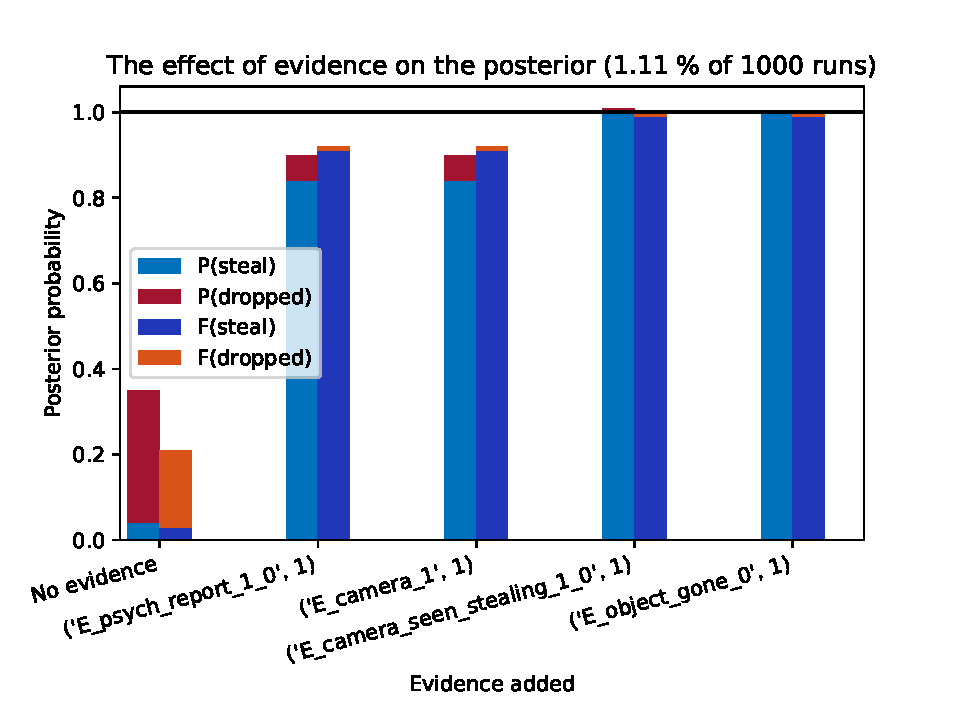
\includegraphics[width=0.7\textwidth]{GroteMarktPrivateEND/plots/freq/evidence_progress_GroteMarktPrivate_1000_1.1100.pdf}}
\caption{Most relevant }
\label{te}
\end{subfigure}
\begin{subfigure}{\textwidth}
\makebox[\textwidth][c]{
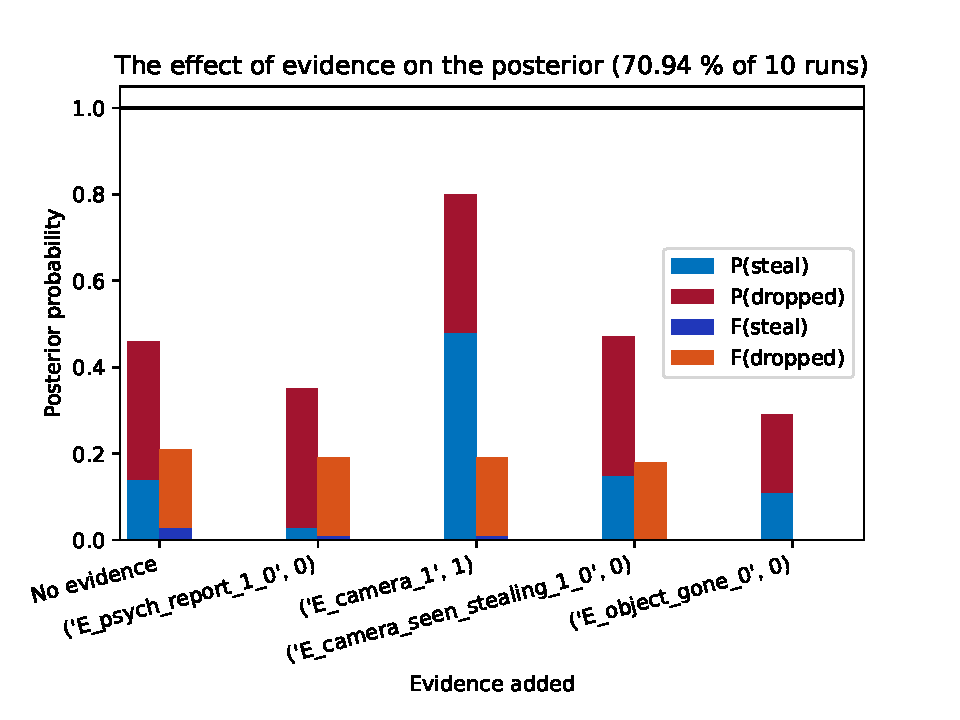
\includegraphics[width=0.7\textwidth]{GroteMarktPrivateEND/plots/freq/evidence_progress_GroteMarktPrivate_10_70.9400.pdf}
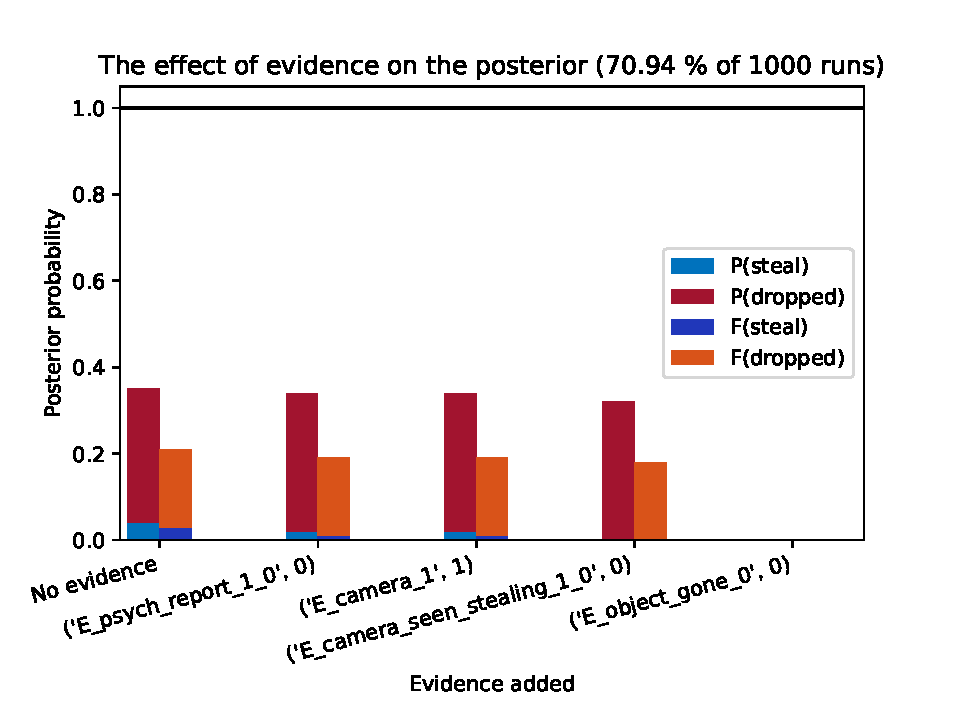
\includegraphics[width=0.7\textwidth]{GroteMarktPrivateEND/plots/freq/evidence_progress_GroteMarktPrivate_1000_70.9400.pdf}}
\caption{Most frequent}
\label{sfb}
\end{subfigure}
\end{center}
\end{figure}



\begin{table}
\begin{center}
\begin{tabular}{|l|c|c|c|}
\hline
evidence & H1 & H2 & H3 \\
\hline
(0, 1, 0, 0)&P(neither) (0.97) & P(dropped) (0.02) & P(steal) (0.01) \\
(0, 1, 0, 1)&P(dropped) (0.96) & P(neither) (0.03) & P(steal) (0.01) \\
(0, 0, 0, 0)&P(neither) (0.97) & P(dropped) (0.02) & P(steal) (0.01) \\
(0, 0, 0, 1)&P(dropped) (0.96) & P(neither) (0.03) & P(steal) (0.01) \\
(0, 1, 1, 1)&P(dropped) (0.96) & P(steal) (0.12) & P(neither) (-0.08) \\
(1, 1, 1, 1)&P(steal) (0.96) & P(dropped) (0.21) & P(neither) (-0.17) \\
(1, 0, 0, 1)&P(steal) (0.59) & P(dropped) (0.21) & P(neither) (0.20) \\
(1, 1, 0, 1)&P(steal) (0.59) & P(dropped) (0.21) & P(neither) (0.20) \\
(0, 1, 1, 0)&P(neither) (0.86) & P(steal) (0.12) & P(dropped) (0.02) \\
(1, 1, 0, 0)&P(dropped) (0.70) & P(steal) (0.59) & P(neither) (-0.29) \\
\hline
\end{tabular}
\end{center}
\caption{ Low number of runs, probability estimates for all cumulative evidence sets for runs =  10}
\label{journal}
\end{table}

\begin{table}[htbp]
\begin{center}
\begin{tabular}{|l|c|c|c|}
\hline
evidence & H1 & H2 & H3 \\
\hline
(0, 1, 0, 0)&P(neither) (1.00) & P(steal) (0.00) & P(dropped) (0.00) \\
(0, 1, 0, 1)&P(dropped) (0.99) & P(steal) (0.01) & P(neither) (0.00) \\
(0, 0, 0, 0)&P(neither) (1.00) & P(steal) (0.00) & P(dropped) (0.00) \\
(0, 0, 0, 1)&P(dropped) (0.95) & P(steal) (0.05) & P(neither) (0.00) \\
(0, 1, 1, 1)&P(steal) (1.00) & P(dropped) (0.01) & P(neither) (-0.01) \\
(1, 1, 1, 1)&P(steal) (1.00) & P(dropped) (0.00) & P(neither) (0.00) \\
(1, 0, 0, 1)&P(steal) (1.00) & P(dropped) (0.01) & P(neither) (-0.01) \\
(1, 1, 0, 1)&P(steal) (0.98) & P(dropped) (0.02) & P(neither) (0.00) \\
(0, 1, 1, 0)&P(steal) (0.41) & P(neither) (0.37) & P(dropped) (0.22) \\
(1, 1, 0, 0)&P(neither) (0.97) & P(steal) (0.02) & P(dropped) (0.01) \\
\hline
\end{tabular}
\end{center}
\caption{ Preference ordering with numbers on Bayesian Network prediction for all evidence states (runs 1000)}
\label{somebody}
\end{table}
\begin{table}[htbp]
\begin{center}
\begin{tabular}{|l|c|c|c|}
\hline
evidence & H1 & H2 & H3 \\
\hline
(0, 1, 0, 0)&F(neither) (1.00) & F(steal) (0.00) & F(dropped) (0.00) \\
(0, 1, 0, 1)&F(dropped) (0.98) & F(steal) (0.02) & F(neither) (0.00) \\
(0, 0, 0, 0)&F(neither) (1.00) & F(steal) (0.00) & F(dropped) (0.00) \\
(0, 0, 0, 1)&F(dropped) (0.94) & F(steal) (0.06) & F(neither) (0.00) \\
(0, 1, 1, 1)&F(steal) (0.95) & F(dropped) (0.05) & F(neither) (0.00) \\
(1, 1, 1, 1)&F(steal) (0.99) & F(dropped) (0.01) & F(neither) (0.00) \\
(1, 0, 0, 1)&F(steal) (1.00) & F(dropped) (0.00) & F(neither) (0.00) \\
(1, 1, 0, 1)&F(steal) (1.00) & F(dropped) (0.00) & F(neither) (0.00) \\
(0, 1, 1, 0)&F(neither) (1.00) & F(steal) (0.00) & F(dropped) (0.00) \\
(1, 1, 0, 0)&F(neither) (1.00) & F(steal) (0.00) & F(dropped) (0.00) \\
\hline
\end{tabular}
\end{center}
\caption{ Preference ordering with numbers for all evidence states on `ground truth' for runs=10000}
\label{heretic}
\end{table}


\newpage



\section{Discussion}
In this section we discuss the success of the method, its generalisability, and future research.


\subsection{Evaluating BNs over all possible evidence states using simulations}
With this method, we can show that we can create BNs that predict output probabilities that correspond to the limiting frequencies of events in the simulation. We see that both the preference ordering as well as the probabilities in the output nodes in Table~\ref{somebody} are near identical to those in Table~\ref{heretic}. This means that the best BN reflects the frequencies in the simulation well, not just on one set of cumulative evidence, but on nearly all sets of cumulative evidence. 

The only evidence set where the BN does not reflect the ground truth, is for the evidence set of (0, 1, 1, 0). This is a situation where the agent is seen stealing, but the object is not gone. In the test data of 10,000 entries, there is never an entry where both stealing and dropping are true. Hence, we find that the BN does not predict the output correctly in this case. 

When less data is available to the K2 algorithm, such as the case where the simulation was run for 10 times (Table~\ref{journal}), we find that the accuracy of the network decreases. This means that the network is less able to predict the right outcome across all possible evidence states.

This method also allows us to see when the BN is assigning probability values to mutually exclusive nodes that violate probabilistic constraints. The joint probability over all three states (steal, drop, neither) can never be greater than 1, which means that none of the probability values of steal, drop, and neither, can be smaller than 0. However, in both Table~\ref{journal}, and Table~\ref{somebody}, we find that P(`neither') can sometimes be smaller than 0. This is also visible in the cumulative probability plots (see Figure~\ref{nobody} where for E\_camera\_seen\_stealing\_1\_0, the joint probability of outcomes $>$ 1). This shows that the mutually exclusive relation between stealing and dropping is not learned correctly in the network. This improves (but is not gone), when the K2 algorithm has access to more data.


This method of evaluating a BN over all states of cumulative evidence can distinguish between better and worse BNs, shows when a BN goes wrong and gives us insight in why that happens. Modellers of data-poor BNs are might think about creating an expected preference ordering on all possible evidence states, before starting to build and test the BN, in order to check whether their BN aligns with their common-sense predictions. If the BN is wrong, this is a sign that either the modeller's estimation is wrong, or that the probabilities as entered in the BN are not correctly representing your actual beliefs.


\subsection{Can a modeller do this?}
Two questions:

Could a person/modeller find these probabilities as found in the network?
think about expert elicitation as discussed in the introduction, could a person do this?
Look at all the nodes
We cannot know this, since the simulation is so far removed from human intuition that subjective probability elicitation will not result in anything useful. 



A user would not be able to say that P(motive) = 0.3 just from the description of the variables in the case study. However, people might be able to guess the CPTs for some nodes (just based on the simulation descriptions). perhaps if the user had the chance to interact with the simulation, they might be able to estimate some frequencies at which events happen. This is something for further research. 

A lighter case: could a person/police/forensic investigators, model something using simulations?
Yes, simulations are a nicer modelling primitive than straight BNs. Could use a true simulation to generate data and cases and train a BN on that, and use decision making based on BN data. A simulation like programmed now is nice as a data-generator, but not so much as a reasoning thing. However, it is unclear unknown difficult to know in what detail one should model for a real case, instead of just a test-case.


Simulations are nice because you do not have to deal with calculating the probabilities yourself. For instance, calculating the probability of motive, means that we need to calculate vulnerable and valuable. This can be done, given that the guy has a target: valuable = (2/5)*(1/2)*(1/2) = 0.1, while vulnerable = (1/5)+(3/5)(1/2) = 0.5. Hence, motive = 0.05, or 5\%, just by bare probability calculations, which matches the probability as found in the network and the training dataset. However, tthis was relatively easy because these were straightforward uniform distributions. This calculation is going to be more complex if we're dealing with either more complex distributions (normals, etc.), or if we do not have a good idea about the underlying distributions. However, doing this using simulations makes it a lot easier, the numbers `just' emerge without any calculation. We even encounter this in the simulation right now: the probability that the camera sees the stealing is very difficult to calculate analytically. Simulations are a more natural way to think about this.The simulation can also easily become more relevant (more like a level 1 or 2 simulation in the taxonomy), by creating more realistic agent motivation models and behaviour. On the other hand, debugging simulation results is really annoying.





\subsection{Evaluating BNs over all possible evidence states using real life}

We applied this method to the network presented in \citet{vanLeeuwen2019}, shown in Figure~\ref{love}.  This network models a crime case where a suspect P murdered a tenant, then fled by car, and later called his parents to confess the crime, which is modelled as scenario 1 (scn1). In his own testimony, P states that he has amnesia and does not remember the day of the murder, and also that he was kidnapped, which is modelled as scenario 2 (scn2). The two scenarios are mutually exclusive and exhaustive. Evidence node names are shortened in table for convenience: `testimony\_amnesia' (TA), `Medical\_investigation\_found\_no\_amnesia' (MA), `testimony\_kidnapping' (TK), `no\_concrete\_evidence\_for\_kidnapping' (NK), `phonecall\_parents' (PP),  `car\_with\_bloodstains\_found' (CB), `body\_found' (BF), `signs\_of\_violence' (SV), `phonecall\_with\_friend'(PF), `testimony\_conflict' (TC), `weapon\_found' (WF).


\begin{figure}[htbp]
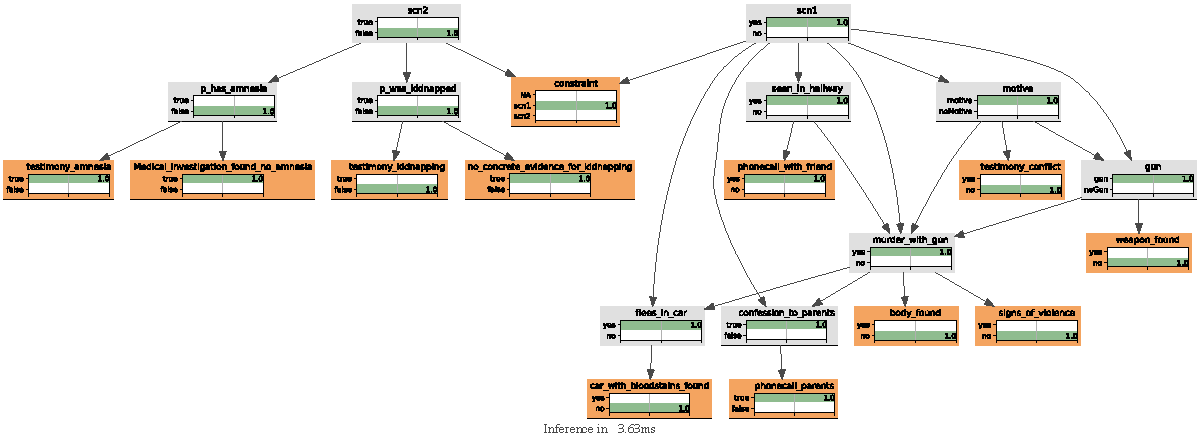
\includegraphics[width=\linewidth]{images/oldnetwork.pdf}
\caption{Example of subjective probability estimation resulting in a guilty verdict for insufficient evidence}
\label{love}
\end{figure}%

This network has 11 evidence nodes, which means a potential of $2^11 = 2048$ total combinations of evidence. Time-technically, this took 7.66 seconds. However, the network constrained some combinations of evidence states, in 56.25\% of evidence states, the combination of evidence was not allowed by virtue of the BN. In the remaining 896 evidence states (see Appendix), the evidence state was applied to the network and the posterior probability for scenario 1 and scenario 2 were calculated.

In general, we find that scenario 1 and scenario 2 are about equally preferred under the states of evidence, in 428 states, scenario 1 has a higher posterior probability, and in 468 states, scenario 2 has a higher posterior. In 768 states of evidence, it is the case that either scenario 1 or scenario 2 is equal to 1, which means that we are fully convinced that that scenario is correct: in half the cases, we fully believe scenario 1, and in the other half, we fully believe scenario 2.

We do not have an automated baseline for this network so that means that if we wanted to assess the validity of the BN, we would have to create a baseline by hand. This would mean that we have to write down our predictions for posteriors or preference ordering for every combination of evidence by hand, and check them against the outcome of the BN. This is very demanding, confusing, and boring. Hence, instead of fully performing the method outlined in this paper, we only show some interesting highlights of where we can see that the network goes wrong, or does something right. These highlights are extracted from the table in the Appendix and placed in Table~\ref{cases} (number corresponds to number in Table~\ref{cases}).


\begin{table}[htbp]
\begin{center}
\begin{tabular}{|l|l|c|c|}
\hline
 & evidence & H1 & H2  \\
\hline
1 & TA, MA, TK, NK, CB, PP, BF, SV, PF, TC, WF & scn1 (1.00) & scn2 (0.00)\\
2 & TA, $\neg$MA, $\neg$TK, $\neg$NK, $\neg$CB, PP, $\neg$BF, $\neg$SV, PF, $\neg$TC, $\neg$WF & scn1 (1.00) & scn2 (0.00)\\
3 & TA, MA, TK, NK, CB, PP, $\neg$BF, $\neg$SV, PF, $\neg$TC, $\neg$WF & scn1 (0.00) & scn2 (1.00)\\
4 & TA, MA, TK, NK, CB, PP, BF, $\neg$SV, PF, $\neg$TC, $\neg$WF & scn1 (0.40) & scn2 (0.60)\\
5 & TA, $\neg$MA, TK, $\neg$NK, $\neg$CB, PP, BF, $\neg$SV, PF, TC, WF & scn1 (0.07) & scn2 (0.93)\\
6 & $\neg$TA, $\neg$MA, $\neg$TK, $\neg$NK, $\neg$CB, $\neg$PP, $\neg$BF, $\neg$SV, $\neg$PF, $\neg$TC, $\neg$WF & None & None\\

\hline
\end{tabular}
\end{center}
\caption{ Interesting rows extracted from complete table}
\label{cases}
\end{table}


\begin{enumerate}
\item We find that, if all evidence nodes are true, which is the situation as found in the court case, the network shows that scenario 1 is the case, and that the suspect is guilty, with a probability of 1. This is the expected output, and corresponds to the outcome of \citet{vanLeeuwen2019}.
\item There is no body, no signs of violence, no car with bloodstains, no evidence of existing conflict. The only evidence that the prosecution has, are two phone calls. The outcome of the network is that the suspect is guilty (P(scn1 = `yes') = 100\%). But the evidence that is entered into this network, would not reasonably support this conclusion. No reasonable arguer would argue that this state of evidence is sufficient for a guilty verdict.
\item Here we fully believe scenario 2, so that the suspect is not guilty. However, all evidence that we have learned about scenario 2 shows that scenario 2 is not true: we have testimony for amnesia, but no medical record of it. We have testimony for kidnapping, but no concrete evidence for kidnapping. This should mean that our posterior belief in scenario 2 should decrease. We also have a little evidence on the side of scenario 1: two phone calls, and a car with bloodstains. This would not be enough for a conviction, but it should be enough that our belief in scenario 1 is not 0.
\item The same case as evidence state in case 3, but now we change our evidence. From not having a body found, we add that we find the body, and we see that our belief in scenario 1 increases, from 0 to 0.40. This is a change of our belief in a reasonable direction given new evidence. The size of the belief-change, from 0 to 0.40, is difficult to assess without a realistic baseline.
\item Here we find that the suspect says that he has amnesia and also that he was kidnapped, and this is supported by the other evidence. This adds support for scenario 2. However, we also find a lot of support for scenario 1: a body, a testimony of conflict, the phone calls, weapon found. Just not the car, and no signs of violence on the scene. Here, my subjective probability estimation machine thinks that, even though scenario 2 has some good evidence going for it, I believe that scenario 1 is more likely than 0.07. Hence, the output does not line up with my expectation.
\item This is a special case: if all evidence nodes are false, the inference engine shows the result that the evidence is altogether incompatible. Since both scenarios are mutually exclusive and exhaustive, this result is sensible and shows that the BN can indeed structure our reasoning.
\end{enumerate}

Even without using a simulation, this method can be used to gain insight in whether the BN conforms to our expectations. We can identify cases where it seems to work correctly, such as case 1) and case 3). In case 1), the output conforms to the one datapoint that we have (given all evidence, the suspect is guilty), the BN makes the same decision as the court. In case 4), we find that the network, in this circumstance, responds sensibly to a change in evidence. However, in case 2), 3) and 5), we find the performance of the network not convincing. In case 2), there is insufficient evidence for scenario 1, yet the network chooses scenario 1. In case 3), there is insufficient evidence for scenario 2, yet the network chooses scenario 2. In case 5), there is support for both scenarios, but the posterior probability for scenario 1 seems (subjectively) too low. Furthermore, we now also know which states are deemed impossible (example: case 6). However, since we do not have a simulation or real-life test-cases, we do not have a way of `objectively' checking whether the network performs correctly or not, and to objectively identify combinations of evidence for which the network is performing badly. We can only do spot-checks and manually search through the output to see if we found anything interesting. Also, if we found a case for which the network performs incorrectly, it is also not clear what we should do with that: how should we change the probabilities in the CPT in order to increase `accuracy'?

It is possible to apply this method to other networks (given that they are produced in an open-access format), to non-systematically check the performance of these networks over all possible evidence valuations. In the networks as considered in the Anjum case study in \citet{vlek2016}, or the Simonshaven case in \citet{Fenton2019}, the evidence nodes are distinguished from the hypothesis nodes. Even without considering the temporality of evidence, we can set the cumulative evidence all at once. However, since we do not have simulations for grounding, or data for grounding, we cannot actually evaluate the networks based on `objective' measures. Manually considering all evidence sets will be even more problematic than before. Instead of 11 nodes, the Simonshaven network has 13 evidence nodes, and the Anjum network has 20 evidence nodes. If we assume that calculating 1 case will take around 0.0037 seconds (as calculated from 7.66 seconds for 2048 entries, this does not hold entirely because it also depends on the number of hypothesis nodes), producing all possible Simonshaven states and posteriors should take $2^{13} = 30$ seconds, which is still reasonable, but the Anjum network would take 64 minutes. That is only considering the automatic calculation of the posteriors, and does not consider the time-complexity of creating a manual or automatic baseline. 





\subsection{Problems}

There are three main problems with this approach that limit its generalisability. These problems are the combinatorial explosion of the evidence states, the implausibilities of finding proper grounding, specifying more than we actually need, and the imprecision of the BN definitions of the random variables in real life.

\begin{enumerate}

\item For this approach, we need to consider all possible evidence states. In the worst case, if we have $e$ evidence states, this means that we have $e^2$ possible evidence states. We would have to define a preference ordering or probability distribution on the output nodes in $2^e$ cases. This is plausible in a network with 4 evidence nodes. However, as we saw in the discussion of the literature, this becomes implausible when there are many evidence nodes. 
This necessarily puts an upper bound on the level of granularity one can model in their network. If our network becomes more detailed in how evidence is represented, the higher the probability that considering all possible evidence states becomes improbable. A rough estimation shows that a 20-evidence-node network will take about an hour, but 20 pieces of evidence are not much in a complex case. Due to exponentiality, a network with 25 evidence nodes would result in 2.3 months of calculations.
There's also the combinatorial explosion, where you would need to define many more cases of evidence than you are actually reasoning with. However, we are already doing this implicitly by using a Bayesian Network for reasoning in the first place. 

\item Due to the simulation approach in this paper, we can establish a statistical ground truth in step 4) of our method. We can create both a joint probability distribution and a preference ordering automatically from the simulation. In real life, this would have to be elicited in some way. Even if we assume that we are not in a combinatorial explosion, we would still need to define either a subjective probability distribution over all possible outcomes, or a preference ordering, and use this as a baseline to test the predictions of our BN against. This involves subjectivity twice: first in defining the preference ordering or probability distribution over outcomes, and second the probabilities that are inputted in the CPTs. Future research might establish how successful people are in estimating preference orderings or probability distributions over output nodes, so that we can use these subjective orderings as a baseline, instead of an ordering generated by frequency data from the simulation. 

As we saw when we applied the method to the network without a simulation, it is not plausible to create a manual baseline, as this would be mind-numbingly boring and consume too much time.  Creating a simulation would mean that the simulation should go beyond one room, and instead model an entire city, all places that the suspect can be all the time. This requires a lot more data and attention than is possible now, and it is also unclear how we would test the validity of the simulation, which would result in all our problems just being shifted up a step (to the simulation level, instead of in the BN). This means that simulations might be a good tool to investigate the methods of BNs, but are not suitable for actually investigating real-life crimes (although they might be usable as a tool for predicting situations - stuff where we have frequency data about.

\item Too much data: in the court case, we are only considering the evidence that we believe is true. We do not have to consider these counterfactual states of evidence, all 895 of them. In a BN, these other 895 cases are 1) specified and 2) must be correct. Isn't this asking too much? Other approaches to reasoning, scenario-based, argumentative or hybrid do not need to fill out the CPTs, there they only need to consider the evidence by itself.


\item More generally, a problem with BNs is that a random variable, which is a function that maps a set of events to a `measurable space'. Informally, in this case, the RV maps an event to either T or F. There are two problems: how we define the set of events that we are mapping (domain), and the validity of the `mapping' function.

\begin{enumerate}
\item \textbf{Defining the domain, or the reference class problem:} Defining the set of events is inherently problematic, and is called `the problem of the reference class' \citep{colyvan2001}. The problem of the reference class is in picking the set of events that belong in the domain. This problem is relevant in both the simulation and the real world.  However it is not as relevant in the simulation because often there is only one interesting/relevant way to interpret the events (eg there are not two equally ``good'' `reference classes' for a node like `sneak\_1\_0'). There is only one relevant class (which is defined with respect to the agent behaviour), and that is the relevant reference class. However, in real life, you cannot know which reference class is the most `relevant' or fair to choose. It is unclear how to get out of this bind, but we know that we do reason pragmatically and informally with the reference class.
\item \textbf{Defining the mapping, and its validity:} This is no problem in the simulation, we know what the methods for determining the probabilities in the nodes are valid (which means that they always correctly reflect the underlying progress that is generating them), because it's literally programmed in this way - directly reflecting the states, we literally just count the frequencies. However, in real life, we might not even know the validity of different possible mappings for the same node. In short, how do we determine in real life that `sneak\_1\_0'? How can we determine if anyone is actually `sneaking', and how will we know if this method of determination is valid? This is also why BNs for forensic-statistical BNs are more legitimate: in these forensic-statistic fields, we have defined clear methods and we know the method through which we are mapping: these variables are operationalised. This is not the case for more `vague' nodes.
\end{enumerate}
\end{enumerate}



\subsection{Conclusion}

\subsubsection{Summary}
 
\subsubsection{Future Research}

The simulation in this paper is not complex, and does not model reality in any realistic way. The purpose of this simulation was just to generate data, and did not need to reflect any specific facts about the world. However, agent-based modelling can be useful for investigating different aspects of Bayesian Networks, or reasoning with evidence more generally. Increasing the level of the simulation from level 0 to something that reflects reality is useful to investigate problems such as the Opportunity Prior as presented in \citet{Fenton2017}. 

\newpage
\bibliographystyle{apalike}
\bibliography{masterThesisCitations}

\newpage
\section*{Appendix}

This table shows the output of the Jurix network on the states that are possible for it. For 56\% of input, the network says that the evidence entered together is not possible, which would represent impossible states. However, this leaves us with too many possible states lol.

'testimony\_amnesia' (TA), 'Medical\_investigation\_found\_no\_amnesia' (MA), 'testimony\_kidnapping' (TK), 'no\_concrete\_evidence\_for\_kidnapping' (NK), 'car\_with\_bloodstains\_found' (CB), 'phonecall\_parents' (PP), 'body\_found' (BF), 'signs\_of\_violence' (SV), 'phonecall\_with\_friend'(PF), 'testimony\_conflict' (TC), 'weapon\_found' (WF).

%\end{document}
%\begin{document}

\begin{longtable}{|l|l|c|c|} 
 \hline 
 case & evidence & scn1 & scn2  \\ 
 \hline 

1 & $\neg$TA, $\neg$MA, $\neg$TK, $\neg$NK, $\neg$CB, PP, $\neg$BF, $\neg$SV, PF, $\neg$TC, $\neg$WF & scn1 (1.00) & scn2 (0.00)\\
2 & $\neg$TA, $\neg$MA, $\neg$TK, $\neg$NK, $\neg$CB, PP, $\neg$BF, $\neg$SV, PF, $\neg$TC, WF & scn1 (1.00) & scn2 (0.00)\\
3 & $\neg$TA, $\neg$MA, $\neg$TK, $\neg$NK, $\neg$CB, PP, $\neg$BF, $\neg$SV, PF, TC, $\neg$WF & scn1 (1.00) & scn2 (0.00)\\
4 & $\neg$TA, $\neg$MA, $\neg$TK, $\neg$NK, $\neg$CB, PP, $\neg$BF, $\neg$SV, PF, TC, WF & scn1 (1.00) & scn2 (0.00)\\
5 & $\neg$TA, $\neg$MA, $\neg$TK, $\neg$NK, $\neg$CB, PP, $\neg$BF, SV, PF, $\neg$TC, $\neg$WF & scn1 (1.00) & scn2 (0.00)\\
6 & $\neg$TA, $\neg$MA, $\neg$TK, $\neg$NK, $\neg$CB, PP, $\neg$BF, SV, PF, $\neg$TC, WF & scn1 (1.00) & scn2 (0.00)\\
7 & $\neg$TA, $\neg$MA, $\neg$TK, $\neg$NK, $\neg$CB, PP, $\neg$BF, SV, PF, TC, $\neg$WF & scn1 (1.00) & scn2 (0.00)\\
8 & $\neg$TA, $\neg$MA, $\neg$TK, $\neg$NK, $\neg$CB, PP, $\neg$BF, SV, PF, TC, WF & scn1 (1.00) & scn2 (0.00)\\
9 & $\neg$TA, $\neg$MA, $\neg$TK, $\neg$NK, $\neg$CB, PP, BF, $\neg$SV, PF, $\neg$TC, $\neg$WF & scn1 (1.00) & scn2 (0.00)\\
10 & $\neg$TA, $\neg$MA, $\neg$TK, $\neg$NK, $\neg$CB, PP, BF, $\neg$SV, PF, $\neg$TC, WF & scn1 (1.00) & scn2 (0.00)\\
11 & $\neg$TA, $\neg$MA, $\neg$TK, $\neg$NK, $\neg$CB, PP, BF, $\neg$SV, PF, TC, $\neg$WF & scn1 (1.00) & scn2 (0.00)\\
12 & $\neg$TA, $\neg$MA, $\neg$TK, $\neg$NK, $\neg$CB, PP, BF, $\neg$SV, PF, TC, WF & scn1 (1.00) & scn2 (0.00)\\
13 & $\neg$TA, $\neg$MA, $\neg$TK, $\neg$NK, $\neg$CB, PP, BF, SV, PF, $\neg$TC, $\neg$WF & scn1 (1.00) & scn2 (0.00)\\
14 & $\neg$TA, $\neg$MA, $\neg$TK, $\neg$NK, $\neg$CB, PP, BF, SV, PF, $\neg$TC, WF & scn1 (1.00) & scn2 (0.00)\\
15 & $\neg$TA, $\neg$MA, $\neg$TK, $\neg$NK, $\neg$CB, PP, BF, SV, PF, TC, $\neg$WF & scn1 (1.00) & scn2 (0.00)\\
16 & $\neg$TA, $\neg$MA, $\neg$TK, $\neg$NK, $\neg$CB, PP, BF, SV, PF, TC, WF & scn1 (1.00) & scn2 (0.00)\\
17 & $\neg$TA, $\neg$MA, $\neg$TK, $\neg$NK, CB, PP, $\neg$BF, $\neg$SV, PF, $\neg$TC, $\neg$WF & scn1 (1.00) & scn2 (0.00)\\
18 & $\neg$TA, $\neg$MA, $\neg$TK, $\neg$NK, CB, PP, $\neg$BF, $\neg$SV, PF, $\neg$TC, WF & scn1 (1.00) & scn2 (0.00)\\
19 & $\neg$TA, $\neg$MA, $\neg$TK, $\neg$NK, CB, PP, $\neg$BF, $\neg$SV, PF, TC, $\neg$WF & scn1 (1.00) & scn2 (0.00)\\
20 & $\neg$TA, $\neg$MA, $\neg$TK, $\neg$NK, CB, PP, $\neg$BF, $\neg$SV, PF, TC, WF & scn1 (1.00) & scn2 (0.00)\\
21 & $\neg$TA, $\neg$MA, $\neg$TK, $\neg$NK, CB, PP, $\neg$BF, SV, PF, $\neg$TC, $\neg$WF & scn1 (1.00) & scn2 (0.00)\\
22 & $\neg$TA, $\neg$MA, $\neg$TK, $\neg$NK, CB, PP, $\neg$BF, SV, PF, $\neg$TC, WF & scn1 (1.00) & scn2 (0.00)\\
23 & $\neg$TA, $\neg$MA, $\neg$TK, $\neg$NK, CB, PP, $\neg$BF, SV, PF, TC, $\neg$WF & scn1 (1.00) & scn2 (0.00)\\
24 & $\neg$TA, $\neg$MA, $\neg$TK, $\neg$NK, CB, PP, $\neg$BF, SV, PF, TC, WF & scn1 (1.00) & scn2 (0.00)\\
25 & $\neg$TA, $\neg$MA, $\neg$TK, $\neg$NK, CB, PP, BF, $\neg$SV, PF, $\neg$TC, $\neg$WF & scn1 (1.00) & scn2 (0.00)\\
26 & $\neg$TA, $\neg$MA, $\neg$TK, $\neg$NK, CB, PP, BF, $\neg$SV, PF, $\neg$TC, WF & scn1 (1.00) & scn2 (0.00)\\
27 & $\neg$TA, $\neg$MA, $\neg$TK, $\neg$NK, CB, PP, BF, $\neg$SV, PF, TC, $\neg$WF & scn1 (1.00) & scn2 (0.00)\\
28 & $\neg$TA, $\neg$MA, $\neg$TK, $\neg$NK, CB, PP, BF, $\neg$SV, PF, TC, WF & scn1 (1.00) & scn2 (0.00)\\
29 & $\neg$TA, $\neg$MA, $\neg$TK, $\neg$NK, CB, PP, BF, SV, PF, $\neg$TC, $\neg$WF & scn1 (1.00) & scn2 (0.00)\\
30 & $\neg$TA, $\neg$MA, $\neg$TK, $\neg$NK, CB, PP, BF, SV, PF, $\neg$TC, WF & scn1 (1.00) & scn2 (0.00)\\
31 & $\neg$TA, $\neg$MA, $\neg$TK, $\neg$NK, CB, PP, BF, SV, PF, TC, $\neg$WF & scn1 (1.00) & scn2 (0.00)\\
32 & $\neg$TA, $\neg$MA, $\neg$TK, $\neg$NK, CB, PP, BF, SV, PF, TC, WF & scn1 (1.00) & scn2 (0.00)\\
33 & $\neg$TA, $\neg$MA, $\neg$TK, NK, $\neg$CB, PP, $\neg$BF, $\neg$SV, PF, $\neg$TC, $\neg$WF & scn1 (1.00) & scn2 (0.00)\\
34 & $\neg$TA, $\neg$MA, $\neg$TK, NK, $\neg$CB, PP, $\neg$BF, $\neg$SV, PF, $\neg$TC, WF & scn1 (1.00) & scn2 (0.00)\\
35 & $\neg$TA, $\neg$MA, $\neg$TK, NK, $\neg$CB, PP, $\neg$BF, $\neg$SV, PF, TC, $\neg$WF & scn1 (1.00) & scn2 (0.00)\\
36 & $\neg$TA, $\neg$MA, $\neg$TK, NK, $\neg$CB, PP, $\neg$BF, $\neg$SV, PF, TC, WF & scn1 (1.00) & scn2 (0.00)\\
37 & $\neg$TA, $\neg$MA, $\neg$TK, NK, $\neg$CB, PP, $\neg$BF, SV, PF, $\neg$TC, $\neg$WF & scn1 (1.00) & scn2 (0.00)\\
38 & $\neg$TA, $\neg$MA, $\neg$TK, NK, $\neg$CB, PP, $\neg$BF, SV, PF, $\neg$TC, WF & scn1 (1.00) & scn2 (0.00)\\
39 & $\neg$TA, $\neg$MA, $\neg$TK, NK, $\neg$CB, PP, $\neg$BF, SV, PF, TC, $\neg$WF & scn1 (1.00) & scn2 (0.00)\\
40 & $\neg$TA, $\neg$MA, $\neg$TK, NK, $\neg$CB, PP, $\neg$BF, SV, PF, TC, WF & scn1 (1.00) & scn2 (0.00)\\
41 & $\neg$TA, $\neg$MA, $\neg$TK, NK, $\neg$CB, PP, BF, $\neg$SV, PF, $\neg$TC, $\neg$WF & scn1 (1.00) & scn2 (0.00)\\
42 & $\neg$TA, $\neg$MA, $\neg$TK, NK, $\neg$CB, PP, BF, $\neg$SV, PF, $\neg$TC, WF & scn1 (1.00) & scn2 (0.00)\\
43 & $\neg$TA, $\neg$MA, $\neg$TK, NK, $\neg$CB, PP, BF, $\neg$SV, PF, TC, $\neg$WF & scn1 (1.00) & scn2 (0.00)\\
44 & $\neg$TA, $\neg$MA, $\neg$TK, NK, $\neg$CB, PP, BF, $\neg$SV, PF, TC, WF & scn1 (1.00) & scn2 (0.00)\\
45 & $\neg$TA, $\neg$MA, $\neg$TK, NK, $\neg$CB, PP, BF, SV, PF, $\neg$TC, $\neg$WF & scn1 (1.00) & scn2 (0.00)\\
46 & $\neg$TA, $\neg$MA, $\neg$TK, NK, $\neg$CB, PP, BF, SV, PF, $\neg$TC, WF & scn1 (1.00) & scn2 (0.00)\\
47 & $\neg$TA, $\neg$MA, $\neg$TK, NK, $\neg$CB, PP, BF, SV, PF, TC, $\neg$WF & scn1 (1.00) & scn2 (0.00)\\
48 & $\neg$TA, $\neg$MA, $\neg$TK, NK, $\neg$CB, PP, BF, SV, PF, TC, WF & scn1 (1.00) & scn2 (0.00)\\
49 & $\neg$TA, $\neg$MA, $\neg$TK, NK, CB, PP, $\neg$BF, $\neg$SV, PF, $\neg$TC, $\neg$WF & scn1 (1.00) & scn2 (0.00)\\
50 & $\neg$TA, $\neg$MA, $\neg$TK, NK, CB, PP, $\neg$BF, $\neg$SV, PF, $\neg$TC, WF & scn1 (1.00) & scn2 (0.00)\\
51 & $\neg$TA, $\neg$MA, $\neg$TK, NK, CB, PP, $\neg$BF, $\neg$SV, PF, TC, $\neg$WF & scn1 (1.00) & scn2 (0.00)\\
52 & $\neg$TA, $\neg$MA, $\neg$TK, NK, CB, PP, $\neg$BF, $\neg$SV, PF, TC, WF & scn1 (1.00) & scn2 (0.00)\\
53 & $\neg$TA, $\neg$MA, $\neg$TK, NK, CB, PP, $\neg$BF, SV, PF, $\neg$TC, $\neg$WF & scn1 (1.00) & scn2 (0.00)\\
54 & $\neg$TA, $\neg$MA, $\neg$TK, NK, CB, PP, $\neg$BF, SV, PF, $\neg$TC, WF & scn1 (1.00) & scn2 (0.00)\\
55 & $\neg$TA, $\neg$MA, $\neg$TK, NK, CB, PP, $\neg$BF, SV, PF, TC, $\neg$WF & scn1 (1.00) & scn2 (0.00)\\
56 & $\neg$TA, $\neg$MA, $\neg$TK, NK, CB, PP, $\neg$BF, SV, PF, TC, WF & scn1 (1.00) & scn2 (0.00)\\
57 & $\neg$TA, $\neg$MA, $\neg$TK, NK, CB, PP, BF, $\neg$SV, PF, $\neg$TC, $\neg$WF & scn1 (1.00) & scn2 (0.00)\\
58 & $\neg$TA, $\neg$MA, $\neg$TK, NK, CB, PP, BF, $\neg$SV, PF, $\neg$TC, WF & scn1 (1.00) & scn2 (0.00)\\
59 & $\neg$TA, $\neg$MA, $\neg$TK, NK, CB, PP, BF, $\neg$SV, PF, TC, $\neg$WF & scn1 (1.00) & scn2 (0.00)\\
60 & $\neg$TA, $\neg$MA, $\neg$TK, NK, CB, PP, BF, $\neg$SV, PF, TC, WF & scn1 (1.00) & scn2 (0.00)\\
61 & $\neg$TA, $\neg$MA, $\neg$TK, NK, CB, PP, BF, SV, PF, $\neg$TC, $\neg$WF & scn1 (1.00) & scn2 (0.00)\\
62 & $\neg$TA, $\neg$MA, $\neg$TK, NK, CB, PP, BF, SV, PF, $\neg$TC, WF & scn1 (1.00) & scn2 (0.00)\\
63 & $\neg$TA, $\neg$MA, $\neg$TK, NK, CB, PP, BF, SV, PF, TC, $\neg$WF & scn1 (1.00) & scn2 (0.00)\\
64 & $\neg$TA, $\neg$MA, $\neg$TK, NK, CB, PP, BF, SV, PF, TC, WF & scn1 (1.00) & scn2 (0.00)\\
65 & $\neg$TA, $\neg$MA, TK, $\neg$NK, $\neg$CB, PP, $\neg$BF, $\neg$SV, PF, $\neg$TC, $\neg$WF & scn1 (1.00) & scn2 (0.00)\\
66 & $\neg$TA, $\neg$MA, TK, $\neg$NK, $\neg$CB, PP, $\neg$BF, $\neg$SV, PF, $\neg$TC, WF & scn1 (1.00) & scn2 (0.00)\\
67 & $\neg$TA, $\neg$MA, TK, $\neg$NK, $\neg$CB, PP, $\neg$BF, $\neg$SV, PF, TC, $\neg$WF & scn1 (1.00) & scn2 (0.00)\\
68 & $\neg$TA, $\neg$MA, TK, $\neg$NK, $\neg$CB, PP, $\neg$BF, $\neg$SV, PF, TC, WF & scn1 (1.00) & scn2 (0.00)\\
69 & $\neg$TA, $\neg$MA, TK, $\neg$NK, $\neg$CB, PP, $\neg$BF, SV, PF, $\neg$TC, $\neg$WF & scn1 (1.00) & scn2 (0.00)\\
70 & $\neg$TA, $\neg$MA, TK, $\neg$NK, $\neg$CB, PP, $\neg$BF, SV, PF, $\neg$TC, WF & scn1 (1.00) & scn2 (0.00)\\
71 & $\neg$TA, $\neg$MA, TK, $\neg$NK, $\neg$CB, PP, $\neg$BF, SV, PF, TC, $\neg$WF & scn1 (1.00) & scn2 (0.00)\\
72 & $\neg$TA, $\neg$MA, TK, $\neg$NK, $\neg$CB, PP, $\neg$BF, SV, PF, TC, WF & scn1 (1.00) & scn2 (0.00)\\
73 & $\neg$TA, $\neg$MA, TK, $\neg$NK, $\neg$CB, PP, BF, $\neg$SV, PF, $\neg$TC, $\neg$WF & scn1 (1.00) & scn2 (0.00)\\
74 & $\neg$TA, $\neg$MA, TK, $\neg$NK, $\neg$CB, PP, BF, $\neg$SV, PF, $\neg$TC, WF & scn1 (1.00) & scn2 (0.00)\\
75 & $\neg$TA, $\neg$MA, TK, $\neg$NK, $\neg$CB, PP, BF, $\neg$SV, PF, TC, $\neg$WF & scn1 (1.00) & scn2 (0.00)\\
76 & $\neg$TA, $\neg$MA, TK, $\neg$NK, $\neg$CB, PP, BF, $\neg$SV, PF, TC, WF & scn1 (1.00) & scn2 (0.00)\\
77 & $\neg$TA, $\neg$MA, TK, $\neg$NK, $\neg$CB, PP, BF, SV, PF, $\neg$TC, $\neg$WF & scn1 (1.00) & scn2 (0.00)\\
78 & $\neg$TA, $\neg$MA, TK, $\neg$NK, $\neg$CB, PP, BF, SV, PF, $\neg$TC, WF & scn1 (1.00) & scn2 (0.00)\\
79 & $\neg$TA, $\neg$MA, TK, $\neg$NK, $\neg$CB, PP, BF, SV, PF, TC, $\neg$WF & scn1 (1.00) & scn2 (0.00)\\
80 & $\neg$TA, $\neg$MA, TK, $\neg$NK, $\neg$CB, PP, BF, SV, PF, TC, WF & scn1 (1.00) & scn2 (0.00)\\
81 & $\neg$TA, $\neg$MA, TK, $\neg$NK, CB, PP, $\neg$BF, $\neg$SV, PF, $\neg$TC, $\neg$WF & scn1 (1.00) & scn2 (0.00)\\
82 & $\neg$TA, $\neg$MA, TK, $\neg$NK, CB, PP, $\neg$BF, $\neg$SV, PF, $\neg$TC, WF & scn1 (1.00) & scn2 (0.00)\\
83 & $\neg$TA, $\neg$MA, TK, $\neg$NK, CB, PP, $\neg$BF, $\neg$SV, PF, TC, $\neg$WF & scn1 (1.00) & scn2 (0.00)\\
84 & $\neg$TA, $\neg$MA, TK, $\neg$NK, CB, PP, $\neg$BF, $\neg$SV, PF, TC, WF & scn1 (1.00) & scn2 (0.00)\\
85 & $\neg$TA, $\neg$MA, TK, $\neg$NK, CB, PP, $\neg$BF, SV, PF, $\neg$TC, $\neg$WF & scn1 (1.00) & scn2 (0.00)\\
86 & $\neg$TA, $\neg$MA, TK, $\neg$NK, CB, PP, $\neg$BF, SV, PF, $\neg$TC, WF & scn1 (1.00) & scn2 (0.00)\\
87 & $\neg$TA, $\neg$MA, TK, $\neg$NK, CB, PP, $\neg$BF, SV, PF, TC, $\neg$WF & scn1 (1.00) & scn2 (0.00)\\
88 & $\neg$TA, $\neg$MA, TK, $\neg$NK, CB, PP, $\neg$BF, SV, PF, TC, WF & scn1 (1.00) & scn2 (0.00)\\
89 & $\neg$TA, $\neg$MA, TK, $\neg$NK, CB, PP, BF, $\neg$SV, PF, $\neg$TC, $\neg$WF & scn1 (1.00) & scn2 (0.00)\\
90 & $\neg$TA, $\neg$MA, TK, $\neg$NK, CB, PP, BF, $\neg$SV, PF, $\neg$TC, WF & scn1 (1.00) & scn2 (0.00)\\
91 & $\neg$TA, $\neg$MA, TK, $\neg$NK, CB, PP, BF, $\neg$SV, PF, TC, $\neg$WF & scn1 (1.00) & scn2 (0.00)\\
92 & $\neg$TA, $\neg$MA, TK, $\neg$NK, CB, PP, BF, $\neg$SV, PF, TC, WF & scn1 (1.00) & scn2 (0.00)\\
93 & $\neg$TA, $\neg$MA, TK, $\neg$NK, CB, PP, BF, SV, PF, $\neg$TC, $\neg$WF & scn1 (1.00) & scn2 (0.00)\\
94 & $\neg$TA, $\neg$MA, TK, $\neg$NK, CB, PP, BF, SV, PF, $\neg$TC, WF & scn1 (1.00) & scn2 (0.00)\\
95 & $\neg$TA, $\neg$MA, TK, $\neg$NK, CB, PP, BF, SV, PF, TC, $\neg$WF & scn1 (1.00) & scn2 (0.00)\\
96 & $\neg$TA, $\neg$MA, TK, $\neg$NK, CB, PP, BF, SV, PF, TC, WF & scn1 (1.00) & scn2 (0.00)\\
97 & $\neg$TA, $\neg$MA, TK, NK, $\neg$CB, PP, $\neg$BF, $\neg$SV, PF, $\neg$TC, $\neg$WF & scn1 (1.00) & scn2 (0.00)\\
98 & $\neg$TA, $\neg$MA, TK, NK, $\neg$CB, PP, $\neg$BF, $\neg$SV, PF, $\neg$TC, WF & scn1 (1.00) & scn2 (0.00)\\
99 & $\neg$TA, $\neg$MA, TK, NK, $\neg$CB, PP, $\neg$BF, $\neg$SV, PF, TC, $\neg$WF & scn1 (1.00) & scn2 (0.00)\\
100 & $\neg$TA, $\neg$MA, TK, NK, $\neg$CB, PP, $\neg$BF, $\neg$SV, PF, TC, WF & scn1 (1.00) & scn2 (0.00)\\
101 & $\neg$TA, $\neg$MA, TK, NK, $\neg$CB, PP, $\neg$BF, SV, PF, $\neg$TC, $\neg$WF & scn1 (1.00) & scn2 (0.00)\\
102 & $\neg$TA, $\neg$MA, TK, NK, $\neg$CB, PP, $\neg$BF, SV, PF, $\neg$TC, WF & scn1 (1.00) & scn2 (0.00)\\
103 & $\neg$TA, $\neg$MA, TK, NK, $\neg$CB, PP, $\neg$BF, SV, PF, TC, $\neg$WF & scn1 (1.00) & scn2 (0.00)\\
104 & $\neg$TA, $\neg$MA, TK, NK, $\neg$CB, PP, $\neg$BF, SV, PF, TC, WF & scn1 (1.00) & scn2 (0.00)\\
105 & $\neg$TA, $\neg$MA, TK, NK, $\neg$CB, PP, BF, $\neg$SV, PF, $\neg$TC, $\neg$WF & scn1 (1.00) & scn2 (0.00)\\
106 & $\neg$TA, $\neg$MA, TK, NK, $\neg$CB, PP, BF, $\neg$SV, PF, $\neg$TC, WF & scn1 (1.00) & scn2 (0.00)\\
107 & $\neg$TA, $\neg$MA, TK, NK, $\neg$CB, PP, BF, $\neg$SV, PF, TC, $\neg$WF & scn1 (1.00) & scn2 (0.00)\\
108 & $\neg$TA, $\neg$MA, TK, NK, $\neg$CB, PP, BF, $\neg$SV, PF, TC, WF & scn1 (1.00) & scn2 (0.00)\\
109 & $\neg$TA, $\neg$MA, TK, NK, $\neg$CB, PP, BF, SV, PF, $\neg$TC, $\neg$WF & scn1 (1.00) & scn2 (0.00)\\
110 & $\neg$TA, $\neg$MA, TK, NK, $\neg$CB, PP, BF, SV, PF, $\neg$TC, WF & scn1 (1.00) & scn2 (0.00)\\
111 & $\neg$TA, $\neg$MA, TK, NK, $\neg$CB, PP, BF, SV, PF, TC, $\neg$WF & scn1 (1.00) & scn2 (0.00)\\
112 & $\neg$TA, $\neg$MA, TK, NK, $\neg$CB, PP, BF, SV, PF, TC, WF & scn1 (1.00) & scn2 (0.00)\\
113 & $\neg$TA, $\neg$MA, TK, NK, CB, PP, $\neg$BF, $\neg$SV, PF, $\neg$TC, $\neg$WF & scn1 (1.00) & scn2 (0.00)\\
114 & $\neg$TA, $\neg$MA, TK, NK, CB, PP, $\neg$BF, $\neg$SV, PF, $\neg$TC, WF & scn1 (1.00) & scn2 (0.00)\\
115 & $\neg$TA, $\neg$MA, TK, NK, CB, PP, $\neg$BF, $\neg$SV, PF, TC, $\neg$WF & scn1 (1.00) & scn2 (0.00)\\
116 & $\neg$TA, $\neg$MA, TK, NK, CB, PP, $\neg$BF, $\neg$SV, PF, TC, WF & scn1 (1.00) & scn2 (0.00)\\
117 & $\neg$TA, $\neg$MA, TK, NK, CB, PP, $\neg$BF, SV, PF, $\neg$TC, $\neg$WF & scn1 (1.00) & scn2 (0.00)\\
118 & $\neg$TA, $\neg$MA, TK, NK, CB, PP, $\neg$BF, SV, PF, $\neg$TC, WF & scn1 (1.00) & scn2 (0.00)\\
119 & $\neg$TA, $\neg$MA, TK, NK, CB, PP, $\neg$BF, SV, PF, TC, $\neg$WF & scn1 (1.00) & scn2 (0.00)\\
120 & $\neg$TA, $\neg$MA, TK, NK, CB, PP, $\neg$BF, SV, PF, TC, WF & scn1 (1.00) & scn2 (0.00)\\
121 & $\neg$TA, $\neg$MA, TK, NK, CB, PP, BF, $\neg$SV, PF, $\neg$TC, $\neg$WF & scn1 (1.00) & scn2 (0.00)\\
122 & $\neg$TA, $\neg$MA, TK, NK, CB, PP, BF, $\neg$SV, PF, $\neg$TC, WF & scn1 (1.00) & scn2 (0.00)\\
123 & $\neg$TA, $\neg$MA, TK, NK, CB, PP, BF, $\neg$SV, PF, TC, $\neg$WF & scn1 (1.00) & scn2 (0.00)\\
124 & $\neg$TA, $\neg$MA, TK, NK, CB, PP, BF, $\neg$SV, PF, TC, WF & scn1 (1.00) & scn2 (0.00)\\
125 & $\neg$TA, $\neg$MA, TK, NK, CB, PP, BF, SV, PF, $\neg$TC, $\neg$WF & scn1 (1.00) & scn2 (0.00)\\
126 & $\neg$TA, $\neg$MA, TK, NK, CB, PP, BF, SV, PF, $\neg$TC, WF & scn1 (1.00) & scn2 (0.00)\\
127 & $\neg$TA, $\neg$MA, TK, NK, CB, PP, BF, SV, PF, TC, $\neg$WF & scn1 (1.00) & scn2 (0.00)\\
128 & $\neg$TA, $\neg$MA, TK, NK, CB, PP, BF, SV, PF, TC, WF & scn1 (1.00) & scn2 (0.00)\\
129 & $\neg$TA, MA, $\neg$TK, $\neg$NK, $\neg$CB, PP, $\neg$BF, $\neg$SV, PF, $\neg$TC, $\neg$WF & scn1 (1.00) & scn2 (0.00)\\
130 & $\neg$TA, MA, $\neg$TK, $\neg$NK, $\neg$CB, PP, $\neg$BF, $\neg$SV, PF, $\neg$TC, WF & scn1 (1.00) & scn2 (0.00)\\
131 & $\neg$TA, MA, $\neg$TK, $\neg$NK, $\neg$CB, PP, $\neg$BF, $\neg$SV, PF, TC, $\neg$WF & scn1 (1.00) & scn2 (0.00)\\
132 & $\neg$TA, MA, $\neg$TK, $\neg$NK, $\neg$CB, PP, $\neg$BF, $\neg$SV, PF, TC, WF & scn1 (1.00) & scn2 (0.00)\\
133 & $\neg$TA, MA, $\neg$TK, $\neg$NK, $\neg$CB, PP, $\neg$BF, SV, PF, $\neg$TC, $\neg$WF & scn1 (1.00) & scn2 (0.00)\\
134 & $\neg$TA, MA, $\neg$TK, $\neg$NK, $\neg$CB, PP, $\neg$BF, SV, PF, $\neg$TC, WF & scn1 (1.00) & scn2 (0.00)\\
135 & $\neg$TA, MA, $\neg$TK, $\neg$NK, $\neg$CB, PP, $\neg$BF, SV, PF, TC, $\neg$WF & scn1 (1.00) & scn2 (0.00)\\
136 & $\neg$TA, MA, $\neg$TK, $\neg$NK, $\neg$CB, PP, $\neg$BF, SV, PF, TC, WF & scn1 (1.00) & scn2 (0.00)\\
137 & $\neg$TA, MA, $\neg$TK, $\neg$NK, $\neg$CB, PP, BF, $\neg$SV, PF, $\neg$TC, $\neg$WF & scn1 (1.00) & scn2 (0.00)\\
138 & $\neg$TA, MA, $\neg$TK, $\neg$NK, $\neg$CB, PP, BF, $\neg$SV, PF, $\neg$TC, WF & scn1 (1.00) & scn2 (0.00)\\
139 & $\neg$TA, MA, $\neg$TK, $\neg$NK, $\neg$CB, PP, BF, $\neg$SV, PF, TC, $\neg$WF & scn1 (1.00) & scn2 (0.00)\\
140 & $\neg$TA, MA, $\neg$TK, $\neg$NK, $\neg$CB, PP, BF, $\neg$SV, PF, TC, WF & scn1 (1.00) & scn2 (0.00)\\
141 & $\neg$TA, MA, $\neg$TK, $\neg$NK, $\neg$CB, PP, BF, SV, PF, $\neg$TC, $\neg$WF & scn1 (1.00) & scn2 (0.00)\\
142 & $\neg$TA, MA, $\neg$TK, $\neg$NK, $\neg$CB, PP, BF, SV, PF, $\neg$TC, WF & scn1 (1.00) & scn2 (0.00)\\
143 & $\neg$TA, MA, $\neg$TK, $\neg$NK, $\neg$CB, PP, BF, SV, PF, TC, $\neg$WF & scn1 (1.00) & scn2 (0.00)\\
144 & $\neg$TA, MA, $\neg$TK, $\neg$NK, $\neg$CB, PP, BF, SV, PF, TC, WF & scn1 (1.00) & scn2 (0.00)\\
145 & $\neg$TA, MA, $\neg$TK, $\neg$NK, CB, PP, $\neg$BF, $\neg$SV, PF, $\neg$TC, $\neg$WF & scn1 (1.00) & scn2 (0.00)\\
146 & $\neg$TA, MA, $\neg$TK, $\neg$NK, CB, PP, $\neg$BF, $\neg$SV, PF, $\neg$TC, WF & scn1 (1.00) & scn2 (0.00)\\
147 & $\neg$TA, MA, $\neg$TK, $\neg$NK, CB, PP, $\neg$BF, $\neg$SV, PF, TC, $\neg$WF & scn1 (1.00) & scn2 (0.00)\\
148 & $\neg$TA, MA, $\neg$TK, $\neg$NK, CB, PP, $\neg$BF, $\neg$SV, PF, TC, WF & scn1 (1.00) & scn2 (0.00)\\
149 & $\neg$TA, MA, $\neg$TK, $\neg$NK, CB, PP, $\neg$BF, SV, PF, $\neg$TC, $\neg$WF & scn1 (1.00) & scn2 (0.00)\\
150 & $\neg$TA, MA, $\neg$TK, $\neg$NK, CB, PP, $\neg$BF, SV, PF, $\neg$TC, WF & scn1 (1.00) & scn2 (0.00)\\
151 & $\neg$TA, MA, $\neg$TK, $\neg$NK, CB, PP, $\neg$BF, SV, PF, TC, $\neg$WF & scn1 (1.00) & scn2 (0.00)\\
152 & $\neg$TA, MA, $\neg$TK, $\neg$NK, CB, PP, $\neg$BF, SV, PF, TC, WF & scn1 (1.00) & scn2 (0.00)\\
153 & $\neg$TA, MA, $\neg$TK, $\neg$NK, CB, PP, BF, $\neg$SV, PF, $\neg$TC, $\neg$WF & scn1 (1.00) & scn2 (0.00)\\
154 & $\neg$TA, MA, $\neg$TK, $\neg$NK, CB, PP, BF, $\neg$SV, PF, $\neg$TC, WF & scn1 (1.00) & scn2 (0.00)\\
155 & $\neg$TA, MA, $\neg$TK, $\neg$NK, CB, PP, BF, $\neg$SV, PF, TC, $\neg$WF & scn1 (1.00) & scn2 (0.00)\\
156 & $\neg$TA, MA, $\neg$TK, $\neg$NK, CB, PP, BF, $\neg$SV, PF, TC, WF & scn1 (1.00) & scn2 (0.00)\\
157 & $\neg$TA, MA, $\neg$TK, $\neg$NK, CB, PP, BF, SV, PF, $\neg$TC, $\neg$WF & scn1 (1.00) & scn2 (0.00)\\
158 & $\neg$TA, MA, $\neg$TK, $\neg$NK, CB, PP, BF, SV, PF, $\neg$TC, WF & scn1 (1.00) & scn2 (0.00)\\
159 & $\neg$TA, MA, $\neg$TK, $\neg$NK, CB, PP, BF, SV, PF, TC, $\neg$WF & scn1 (1.00) & scn2 (0.00)\\
160 & $\neg$TA, MA, $\neg$TK, $\neg$NK, CB, PP, BF, SV, PF, TC, WF & scn1 (1.00) & scn2 (0.00)\\
161 & $\neg$TA, MA, $\neg$TK, NK, $\neg$CB, PP, $\neg$BF, $\neg$SV, PF, $\neg$TC, $\neg$WF & scn1 (1.00) & scn2 (0.00)\\
162 & $\neg$TA, MA, $\neg$TK, NK, $\neg$CB, PP, $\neg$BF, $\neg$SV, PF, $\neg$TC, WF & scn1 (1.00) & scn2 (0.00)\\
163 & $\neg$TA, MA, $\neg$TK, NK, $\neg$CB, PP, $\neg$BF, $\neg$SV, PF, TC, $\neg$WF & scn1 (1.00) & scn2 (0.00)\\
164 & $\neg$TA, MA, $\neg$TK, NK, $\neg$CB, PP, $\neg$BF, $\neg$SV, PF, TC, WF & scn1 (1.00) & scn2 (0.00)\\
165 & $\neg$TA, MA, $\neg$TK, NK, $\neg$CB, PP, $\neg$BF, SV, PF, $\neg$TC, $\neg$WF & scn1 (1.00) & scn2 (0.00)\\
166 & $\neg$TA, MA, $\neg$TK, NK, $\neg$CB, PP, $\neg$BF, SV, PF, $\neg$TC, WF & scn1 (1.00) & scn2 (0.00)\\
167 & $\neg$TA, MA, $\neg$TK, NK, $\neg$CB, PP, $\neg$BF, SV, PF, TC, $\neg$WF & scn1 (1.00) & scn2 (0.00)\\
168 & $\neg$TA, MA, $\neg$TK, NK, $\neg$CB, PP, $\neg$BF, SV, PF, TC, WF & scn1 (1.00) & scn2 (0.00)\\
169 & $\neg$TA, MA, $\neg$TK, NK, $\neg$CB, PP, BF, $\neg$SV, PF, $\neg$TC, $\neg$WF & scn1 (1.00) & scn2 (0.00)\\
170 & $\neg$TA, MA, $\neg$TK, NK, $\neg$CB, PP, BF, $\neg$SV, PF, $\neg$TC, WF & scn1 (1.00) & scn2 (0.00)\\
171 & $\neg$TA, MA, $\neg$TK, NK, $\neg$CB, PP, BF, $\neg$SV, PF, TC, $\neg$WF & scn1 (1.00) & scn2 (0.00)\\
172 & $\neg$TA, MA, $\neg$TK, NK, $\neg$CB, PP, BF, $\neg$SV, PF, TC, WF & scn1 (1.00) & scn2 (0.00)\\
173 & $\neg$TA, MA, $\neg$TK, NK, $\neg$CB, PP, BF, SV, PF, $\neg$TC, $\neg$WF & scn1 (1.00) & scn2 (0.00)\\
174 & $\neg$TA, MA, $\neg$TK, NK, $\neg$CB, PP, BF, SV, PF, $\neg$TC, WF & scn1 (1.00) & scn2 (0.00)\\
175 & $\neg$TA, MA, $\neg$TK, NK, $\neg$CB, PP, BF, SV, PF, TC, $\neg$WF & scn1 (1.00) & scn2 (0.00)\\
176 & $\neg$TA, MA, $\neg$TK, NK, $\neg$CB, PP, BF, SV, PF, TC, WF & scn1 (1.00) & scn2 (0.00)\\
177 & $\neg$TA, MA, $\neg$TK, NK, CB, PP, $\neg$BF, $\neg$SV, PF, $\neg$TC, $\neg$WF & scn1 (1.00) & scn2 (0.00)\\
178 & $\neg$TA, MA, $\neg$TK, NK, CB, PP, $\neg$BF, $\neg$SV, PF, $\neg$TC, WF & scn1 (1.00) & scn2 (0.00)\\
179 & $\neg$TA, MA, $\neg$TK, NK, CB, PP, $\neg$BF, $\neg$SV, PF, TC, $\neg$WF & scn1 (1.00) & scn2 (0.00)\\
180 & $\neg$TA, MA, $\neg$TK, NK, CB, PP, $\neg$BF, $\neg$SV, PF, TC, WF & scn1 (1.00) & scn2 (0.00)\\
181 & $\neg$TA, MA, $\neg$TK, NK, CB, PP, $\neg$BF, SV, PF, $\neg$TC, $\neg$WF & scn1 (1.00) & scn2 (0.00)\\
182 & $\neg$TA, MA, $\neg$TK, NK, CB, PP, $\neg$BF, SV, PF, $\neg$TC, WF & scn1 (1.00) & scn2 (0.00)\\
183 & $\neg$TA, MA, $\neg$TK, NK, CB, PP, $\neg$BF, SV, PF, TC, $\neg$WF & scn1 (1.00) & scn2 (0.00)\\
184 & $\neg$TA, MA, $\neg$TK, NK, CB, PP, $\neg$BF, SV, PF, TC, WF & scn1 (1.00) & scn2 (0.00)\\
185 & $\neg$TA, MA, $\neg$TK, NK, CB, PP, BF, $\neg$SV, PF, $\neg$TC, $\neg$WF & scn1 (1.00) & scn2 (0.00)\\
186 & $\neg$TA, MA, $\neg$TK, NK, CB, PP, BF, $\neg$SV, PF, $\neg$TC, WF & scn1 (1.00) & scn2 (0.00)\\
187 & $\neg$TA, MA, $\neg$TK, NK, CB, PP, BF, $\neg$SV, PF, TC, $\neg$WF & scn1 (1.00) & scn2 (0.00)\\
188 & $\neg$TA, MA, $\neg$TK, NK, CB, PP, BF, $\neg$SV, PF, TC, WF & scn1 (1.00) & scn2 (0.00)\\
189 & $\neg$TA, MA, $\neg$TK, NK, CB, PP, BF, SV, PF, $\neg$TC, $\neg$WF & scn1 (1.00) & scn2 (0.00)\\
190 & $\neg$TA, MA, $\neg$TK, NK, CB, PP, BF, SV, PF, $\neg$TC, WF & scn1 (1.00) & scn2 (0.00)\\
191 & $\neg$TA, MA, $\neg$TK, NK, CB, PP, BF, SV, PF, TC, $\neg$WF & scn1 (1.00) & scn2 (0.00)\\
192 & $\neg$TA, MA, $\neg$TK, NK, CB, PP, BF, SV, PF, TC, WF & scn1 (1.00) & scn2 (0.00)\\
193 & $\neg$TA, MA, TK, $\neg$NK, $\neg$CB, PP, $\neg$BF, $\neg$SV, PF, $\neg$TC, $\neg$WF & scn1 (1.00) & scn2 (0.00)\\
194 & $\neg$TA, MA, TK, $\neg$NK, $\neg$CB, PP, $\neg$BF, $\neg$SV, PF, $\neg$TC, WF & scn1 (1.00) & scn2 (0.00)\\
195 & $\neg$TA, MA, TK, $\neg$NK, $\neg$CB, PP, $\neg$BF, $\neg$SV, PF, TC, $\neg$WF & scn1 (1.00) & scn2 (0.00)\\
196 & $\neg$TA, MA, TK, $\neg$NK, $\neg$CB, PP, $\neg$BF, $\neg$SV, PF, TC, WF & scn1 (1.00) & scn2 (0.00)\\
197 & $\neg$TA, MA, TK, $\neg$NK, $\neg$CB, PP, $\neg$BF, SV, PF, $\neg$TC, $\neg$WF & scn1 (1.00) & scn2 (0.00)\\
198 & $\neg$TA, MA, TK, $\neg$NK, $\neg$CB, PP, $\neg$BF, SV, PF, $\neg$TC, WF & scn1 (1.00) & scn2 (0.00)\\
199 & $\neg$TA, MA, TK, $\neg$NK, $\neg$CB, PP, $\neg$BF, SV, PF, TC, $\neg$WF & scn1 (1.00) & scn2 (0.00)\\
200 & $\neg$TA, MA, TK, $\neg$NK, $\neg$CB, PP, $\neg$BF, SV, PF, TC, WF & scn1 (1.00) & scn2 (0.00)\\
201 & $\neg$TA, MA, TK, $\neg$NK, $\neg$CB, PP, BF, $\neg$SV, PF, $\neg$TC, $\neg$WF & scn1 (1.00) & scn2 (0.00)\\
202 & $\neg$TA, MA, TK, $\neg$NK, $\neg$CB, PP, BF, $\neg$SV, PF, $\neg$TC, WF & scn1 (1.00) & scn2 (0.00)\\
203 & $\neg$TA, MA, TK, $\neg$NK, $\neg$CB, PP, BF, $\neg$SV, PF, TC, $\neg$WF & scn1 (1.00) & scn2 (0.00)\\
204 & $\neg$TA, MA, TK, $\neg$NK, $\neg$CB, PP, BF, $\neg$SV, PF, TC, WF & scn1 (1.00) & scn2 (0.00)\\
205 & $\neg$TA, MA, TK, $\neg$NK, $\neg$CB, PP, BF, SV, PF, $\neg$TC, $\neg$WF & scn1 (1.00) & scn2 (0.00)\\
206 & $\neg$TA, MA, TK, $\neg$NK, $\neg$CB, PP, BF, SV, PF, $\neg$TC, WF & scn1 (1.00) & scn2 (0.00)\\
207 & $\neg$TA, MA, TK, $\neg$NK, $\neg$CB, PP, BF, SV, PF, TC, $\neg$WF & scn1 (1.00) & scn2 (0.00)\\
208 & $\neg$TA, MA, TK, $\neg$NK, $\neg$CB, PP, BF, SV, PF, TC, WF & scn1 (1.00) & scn2 (0.00)\\
209 & $\neg$TA, MA, TK, $\neg$NK, CB, PP, $\neg$BF, $\neg$SV, PF, $\neg$TC, $\neg$WF & scn1 (1.00) & scn2 (0.00)\\
210 & $\neg$TA, MA, TK, $\neg$NK, CB, PP, $\neg$BF, $\neg$SV, PF, $\neg$TC, WF & scn1 (1.00) & scn2 (0.00)\\
211 & $\neg$TA, MA, TK, $\neg$NK, CB, PP, $\neg$BF, $\neg$SV, PF, TC, $\neg$WF & scn1 (1.00) & scn2 (0.00)\\
212 & $\neg$TA, MA, TK, $\neg$NK, CB, PP, $\neg$BF, $\neg$SV, PF, TC, WF & scn1 (1.00) & scn2 (0.00)\\
213 & $\neg$TA, MA, TK, $\neg$NK, CB, PP, $\neg$BF, SV, PF, $\neg$TC, $\neg$WF & scn1 (1.00) & scn2 (0.00)\\
214 & $\neg$TA, MA, TK, $\neg$NK, CB, PP, $\neg$BF, SV, PF, $\neg$TC, WF & scn1 (1.00) & scn2 (0.00)\\
215 & $\neg$TA, MA, TK, $\neg$NK, CB, PP, $\neg$BF, SV, PF, TC, $\neg$WF & scn1 (1.00) & scn2 (0.00)\\
216 & $\neg$TA, MA, TK, $\neg$NK, CB, PP, $\neg$BF, SV, PF, TC, WF & scn1 (1.00) & scn2 (0.00)\\
217 & $\neg$TA, MA, TK, $\neg$NK, CB, PP, BF, $\neg$SV, PF, $\neg$TC, $\neg$WF & scn1 (1.00) & scn2 (0.00)\\
218 & $\neg$TA, MA, TK, $\neg$NK, CB, PP, BF, $\neg$SV, PF, $\neg$TC, WF & scn1 (1.00) & scn2 (0.00)\\
219 & $\neg$TA, MA, TK, $\neg$NK, CB, PP, BF, $\neg$SV, PF, TC, $\neg$WF & scn1 (1.00) & scn2 (0.00)\\
220 & $\neg$TA, MA, TK, $\neg$NK, CB, PP, BF, $\neg$SV, PF, TC, WF & scn1 (1.00) & scn2 (0.00)\\
221 & $\neg$TA, MA, TK, $\neg$NK, CB, PP, BF, SV, PF, $\neg$TC, $\neg$WF & scn1 (1.00) & scn2 (0.00)\\
222 & $\neg$TA, MA, TK, $\neg$NK, CB, PP, BF, SV, PF, $\neg$TC, WF & scn1 (1.00) & scn2 (0.00)\\
223 & $\neg$TA, MA, TK, $\neg$NK, CB, PP, BF, SV, PF, TC, $\neg$WF & scn1 (1.00) & scn2 (0.00)\\
224 & $\neg$TA, MA, TK, $\neg$NK, CB, PP, BF, SV, PF, TC, WF & scn1 (1.00) & scn2 (0.00)\\
225 & $\neg$TA, MA, TK, NK, $\neg$CB, PP, $\neg$BF, $\neg$SV, PF, $\neg$TC, $\neg$WF & scn1 (1.00) & scn2 (0.00)\\
226 & $\neg$TA, MA, TK, NK, $\neg$CB, PP, $\neg$BF, $\neg$SV, PF, $\neg$TC, WF & scn1 (1.00) & scn2 (0.00)\\
227 & $\neg$TA, MA, TK, NK, $\neg$CB, PP, $\neg$BF, $\neg$SV, PF, TC, $\neg$WF & scn1 (1.00) & scn2 (0.00)\\
228 & $\neg$TA, MA, TK, NK, $\neg$CB, PP, $\neg$BF, $\neg$SV, PF, TC, WF & scn1 (1.00) & scn2 (0.00)\\
229 & $\neg$TA, MA, TK, NK, $\neg$CB, PP, $\neg$BF, SV, PF, $\neg$TC, $\neg$WF & scn1 (1.00) & scn2 (0.00)\\
230 & $\neg$TA, MA, TK, NK, $\neg$CB, PP, $\neg$BF, SV, PF, $\neg$TC, WF & scn1 (1.00) & scn2 (0.00)\\
231 & $\neg$TA, MA, TK, NK, $\neg$CB, PP, $\neg$BF, SV, PF, TC, $\neg$WF & scn1 (1.00) & scn2 (0.00)\\
232 & $\neg$TA, MA, TK, NK, $\neg$CB, PP, $\neg$BF, SV, PF, TC, WF & scn1 (1.00) & scn2 (0.00)\\
233 & $\neg$TA, MA, TK, NK, $\neg$CB, PP, BF, $\neg$SV, PF, $\neg$TC, $\neg$WF & scn1 (1.00) & scn2 (0.00)\\
234 & $\neg$TA, MA, TK, NK, $\neg$CB, PP, BF, $\neg$SV, PF, $\neg$TC, WF & scn1 (1.00) & scn2 (0.00)\\
235 & $\neg$TA, MA, TK, NK, $\neg$CB, PP, BF, $\neg$SV, PF, TC, $\neg$WF & scn1 (1.00) & scn2 (0.00)\\
236 & $\neg$TA, MA, TK, NK, $\neg$CB, PP, BF, $\neg$SV, PF, TC, WF & scn1 (1.00) & scn2 (0.00)\\
237 & $\neg$TA, MA, TK, NK, $\neg$CB, PP, BF, SV, PF, $\neg$TC, $\neg$WF & scn1 (1.00) & scn2 (0.00)\\
238 & $\neg$TA, MA, TK, NK, $\neg$CB, PP, BF, SV, PF, $\neg$TC, WF & scn1 (1.00) & scn2 (0.00)\\
239 & $\neg$TA, MA, TK, NK, $\neg$CB, PP, BF, SV, PF, TC, $\neg$WF & scn1 (1.00) & scn2 (0.00)\\
240 & $\neg$TA, MA, TK, NK, $\neg$CB, PP, BF, SV, PF, TC, WF & scn1 (1.00) & scn2 (0.00)\\
241 & $\neg$TA, MA, TK, NK, CB, PP, $\neg$BF, $\neg$SV, PF, $\neg$TC, $\neg$WF & scn1 (1.00) & scn2 (0.00)\\
242 & $\neg$TA, MA, TK, NK, CB, PP, $\neg$BF, $\neg$SV, PF, $\neg$TC, WF & scn1 (1.00) & scn2 (0.00)\\
243 & $\neg$TA, MA, TK, NK, CB, PP, $\neg$BF, $\neg$SV, PF, TC, $\neg$WF & scn1 (1.00) & scn2 (0.00)\\
244 & $\neg$TA, MA, TK, NK, CB, PP, $\neg$BF, $\neg$SV, PF, TC, WF & scn1 (1.00) & scn2 (0.00)\\
245 & $\neg$TA, MA, TK, NK, CB, PP, $\neg$BF, SV, PF, $\neg$TC, $\neg$WF & scn1 (1.00) & scn2 (0.00)\\
246 & $\neg$TA, MA, TK, NK, CB, PP, $\neg$BF, SV, PF, $\neg$TC, WF & scn1 (1.00) & scn2 (0.00)\\
247 & $\neg$TA, MA, TK, NK, CB, PP, $\neg$BF, SV, PF, TC, $\neg$WF & scn1 (1.00) & scn2 (0.00)\\
248 & $\neg$TA, MA, TK, NK, CB, PP, $\neg$BF, SV, PF, TC, WF & scn1 (1.00) & scn2 (0.00)\\
249 & $\neg$TA, MA, TK, NK, CB, PP, BF, $\neg$SV, PF, $\neg$TC, $\neg$WF & scn1 (1.00) & scn2 (0.00)\\
250 & $\neg$TA, MA, TK, NK, CB, PP, BF, $\neg$SV, PF, $\neg$TC, WF & scn1 (1.00) & scn2 (0.00)\\
251 & $\neg$TA, MA, TK, NK, CB, PP, BF, $\neg$SV, PF, TC, $\neg$WF & scn1 (1.00) & scn2 (0.00)\\
252 & $\neg$TA, MA, TK, NK, CB, PP, BF, $\neg$SV, PF, TC, WF & scn1 (1.00) & scn2 (0.00)\\
253 & $\neg$TA, MA, TK, NK, CB, PP, BF, SV, PF, $\neg$TC, $\neg$WF & scn1 (1.00) & scn2 (0.00)\\
254 & $\neg$TA, MA, TK, NK, CB, PP, BF, SV, PF, $\neg$TC, WF & scn1 (1.00) & scn2 (0.00)\\
255 & $\neg$TA, MA, TK, NK, CB, PP, BF, SV, PF, TC, $\neg$WF & scn1 (1.00) & scn2 (0.00)\\
256 & $\neg$TA, MA, TK, NK, CB, PP, BF, SV, PF, TC, WF & scn1 (1.00) & scn2 (0.00)\\
257 & TA, $\neg$MA, $\neg$TK, $\neg$NK, $\neg$CB, PP, $\neg$BF, $\neg$SV, PF, $\neg$TC, $\neg$WF & scn1 (1.00) & scn2 (0.00)\\
258 & TA, $\neg$MA, $\neg$TK, $\neg$NK, $\neg$CB, PP, $\neg$BF, $\neg$SV, PF, $\neg$TC, WF & scn1 (1.00) & scn2 (0.00)\\
259 & TA, $\neg$MA, $\neg$TK, $\neg$NK, $\neg$CB, PP, $\neg$BF, $\neg$SV, PF, TC, $\neg$WF & scn1 (1.00) & scn2 (0.00)\\
260 & TA, $\neg$MA, $\neg$TK, $\neg$NK, $\neg$CB, PP, $\neg$BF, $\neg$SV, PF, TC, WF & scn1 (1.00) & scn2 (0.00)\\
261 & TA, $\neg$MA, $\neg$TK, $\neg$NK, $\neg$CB, PP, $\neg$BF, SV, PF, $\neg$TC, $\neg$WF & scn1 (1.00) & scn2 (0.00)\\
262 & TA, $\neg$MA, $\neg$TK, $\neg$NK, $\neg$CB, PP, $\neg$BF, SV, PF, $\neg$TC, WF & scn1 (1.00) & scn2 (0.00)\\
263 & TA, $\neg$MA, $\neg$TK, $\neg$NK, $\neg$CB, PP, $\neg$BF, SV, PF, TC, $\neg$WF & scn1 (1.00) & scn2 (0.00)\\
264 & TA, $\neg$MA, $\neg$TK, $\neg$NK, $\neg$CB, PP, $\neg$BF, SV, PF, TC, WF & scn1 (1.00) & scn2 (0.00)\\
265 & TA, $\neg$MA, $\neg$TK, $\neg$NK, $\neg$CB, PP, BF, $\neg$SV, PF, $\neg$TC, $\neg$WF & scn1 (1.00) & scn2 (0.00)\\
266 & TA, $\neg$MA, $\neg$TK, $\neg$NK, $\neg$CB, PP, BF, $\neg$SV, PF, $\neg$TC, WF & scn1 (1.00) & scn2 (0.00)\\
267 & TA, $\neg$MA, $\neg$TK, $\neg$NK, $\neg$CB, PP, BF, $\neg$SV, PF, TC, $\neg$WF & scn1 (1.00) & scn2 (0.00)\\
268 & TA, $\neg$MA, $\neg$TK, $\neg$NK, $\neg$CB, PP, BF, $\neg$SV, PF, TC, WF & scn1 (1.00) & scn2 (0.00)\\
269 & TA, $\neg$MA, $\neg$TK, $\neg$NK, $\neg$CB, PP, BF, SV, PF, $\neg$TC, $\neg$WF & scn1 (1.00) & scn2 (0.00)\\
270 & TA, $\neg$MA, $\neg$TK, $\neg$NK, $\neg$CB, PP, BF, SV, PF, $\neg$TC, WF & scn1 (1.00) & scn2 (0.00)\\
271 & TA, $\neg$MA, $\neg$TK, $\neg$NK, $\neg$CB, PP, BF, SV, PF, TC, $\neg$WF & scn1 (1.00) & scn2 (0.00)\\
272 & TA, $\neg$MA, $\neg$TK, $\neg$NK, $\neg$CB, PP, BF, SV, PF, TC, WF & scn1 (1.00) & scn2 (0.00)\\
273 & TA, $\neg$MA, $\neg$TK, $\neg$NK, CB, PP, $\neg$BF, $\neg$SV, PF, $\neg$TC, $\neg$WF & scn1 (1.00) & scn2 (0.00)\\
274 & TA, $\neg$MA, $\neg$TK, $\neg$NK, CB, PP, $\neg$BF, $\neg$SV, PF, $\neg$TC, WF & scn1 (1.00) & scn2 (0.00)\\
275 & TA, $\neg$MA, $\neg$TK, $\neg$NK, CB, PP, $\neg$BF, $\neg$SV, PF, TC, $\neg$WF & scn1 (1.00) & scn2 (0.00)\\
276 & TA, $\neg$MA, $\neg$TK, $\neg$NK, CB, PP, $\neg$BF, $\neg$SV, PF, TC, WF & scn1 (1.00) & scn2 (0.00)\\
277 & TA, $\neg$MA, $\neg$TK, $\neg$NK, CB, PP, $\neg$BF, SV, PF, $\neg$TC, $\neg$WF & scn1 (1.00) & scn2 (0.00)\\
278 & TA, $\neg$MA, $\neg$TK, $\neg$NK, CB, PP, $\neg$BF, SV, PF, $\neg$TC, WF & scn1 (1.00) & scn2 (0.00)\\
279 & TA, $\neg$MA, $\neg$TK, $\neg$NK, CB, PP, $\neg$BF, SV, PF, TC, $\neg$WF & scn1 (1.00) & scn2 (0.00)\\
280 & TA, $\neg$MA, $\neg$TK, $\neg$NK, CB, PP, $\neg$BF, SV, PF, TC, WF & scn1 (1.00) & scn2 (0.00)\\
281 & TA, $\neg$MA, $\neg$TK, $\neg$NK, CB, PP, BF, $\neg$SV, PF, $\neg$TC, $\neg$WF & scn1 (1.00) & scn2 (0.00)\\
282 & TA, $\neg$MA, $\neg$TK, $\neg$NK, CB, PP, BF, $\neg$SV, PF, $\neg$TC, WF & scn1 (1.00) & scn2 (0.00)\\
283 & TA, $\neg$MA, $\neg$TK, $\neg$NK, CB, PP, BF, $\neg$SV, PF, TC, $\neg$WF & scn1 (1.00) & scn2 (0.00)\\
284 & TA, $\neg$MA, $\neg$TK, $\neg$NK, CB, PP, BF, $\neg$SV, PF, TC, WF & scn1 (1.00) & scn2 (0.00)\\
285 & TA, $\neg$MA, $\neg$TK, $\neg$NK, CB, PP, BF, SV, PF, $\neg$TC, $\neg$WF & scn1 (1.00) & scn2 (0.00)\\
286 & TA, $\neg$MA, $\neg$TK, $\neg$NK, CB, PP, BF, SV, PF, $\neg$TC, WF & scn1 (1.00) & scn2 (0.00)\\
287 & TA, $\neg$MA, $\neg$TK, $\neg$NK, CB, PP, BF, SV, PF, TC, $\neg$WF & scn1 (1.00) & scn2 (0.00)\\
288 & TA, $\neg$MA, $\neg$TK, $\neg$NK, CB, PP, BF, SV, PF, TC, WF & scn1 (1.00) & scn2 (0.00)\\
289 & TA, $\neg$MA, $\neg$TK, NK, $\neg$CB, PP, $\neg$BF, $\neg$SV, PF, $\neg$TC, $\neg$WF & scn1 (1.00) & scn2 (0.00)\\
290 & TA, $\neg$MA, $\neg$TK, NK, $\neg$CB, PP, $\neg$BF, $\neg$SV, PF, $\neg$TC, WF & scn1 (1.00) & scn2 (0.00)\\
291 & TA, $\neg$MA, $\neg$TK, NK, $\neg$CB, PP, $\neg$BF, $\neg$SV, PF, TC, $\neg$WF & scn1 (1.00) & scn2 (0.00)\\
292 & TA, $\neg$MA, $\neg$TK, NK, $\neg$CB, PP, $\neg$BF, $\neg$SV, PF, TC, WF & scn1 (1.00) & scn2 (0.00)\\
293 & TA, $\neg$MA, $\neg$TK, NK, $\neg$CB, PP, $\neg$BF, SV, PF, $\neg$TC, $\neg$WF & scn1 (1.00) & scn2 (0.00)\\
294 & TA, $\neg$MA, $\neg$TK, NK, $\neg$CB, PP, $\neg$BF, SV, PF, $\neg$TC, WF & scn1 (1.00) & scn2 (0.00)\\
295 & TA, $\neg$MA, $\neg$TK, NK, $\neg$CB, PP, $\neg$BF, SV, PF, TC, $\neg$WF & scn1 (1.00) & scn2 (0.00)\\
296 & TA, $\neg$MA, $\neg$TK, NK, $\neg$CB, PP, $\neg$BF, SV, PF, TC, WF & scn1 (1.00) & scn2 (0.00)\\
297 & TA, $\neg$MA, $\neg$TK, NK, $\neg$CB, PP, BF, $\neg$SV, PF, $\neg$TC, $\neg$WF & scn1 (1.00) & scn2 (0.00)\\
298 & TA, $\neg$MA, $\neg$TK, NK, $\neg$CB, PP, BF, $\neg$SV, PF, $\neg$TC, WF & scn1 (1.00) & scn2 (0.00)\\
299 & TA, $\neg$MA, $\neg$TK, NK, $\neg$CB, PP, BF, $\neg$SV, PF, TC, $\neg$WF & scn1 (1.00) & scn2 (0.00)\\
300 & TA, $\neg$MA, $\neg$TK, NK, $\neg$CB, PP, BF, $\neg$SV, PF, TC, WF & scn1 (1.00) & scn2 (0.00)\\
301 & TA, $\neg$MA, $\neg$TK, NK, $\neg$CB, PP, BF, SV, PF, $\neg$TC, $\neg$WF & scn1 (1.00) & scn2 (0.00)\\
302 & TA, $\neg$MA, $\neg$TK, NK, $\neg$CB, PP, BF, SV, PF, $\neg$TC, WF & scn1 (1.00) & scn2 (0.00)\\
303 & TA, $\neg$MA, $\neg$TK, NK, $\neg$CB, PP, BF, SV, PF, TC, $\neg$WF & scn1 (1.00) & scn2 (0.00)\\
304 & TA, $\neg$MA, $\neg$TK, NK, $\neg$CB, PP, BF, SV, PF, TC, WF & scn1 (1.00) & scn2 (0.00)\\
305 & TA, $\neg$MA, $\neg$TK, NK, CB, PP, $\neg$BF, $\neg$SV, PF, $\neg$TC, $\neg$WF & scn1 (1.00) & scn2 (0.00)\\
306 & TA, $\neg$MA, $\neg$TK, NK, CB, PP, $\neg$BF, $\neg$SV, PF, $\neg$TC, WF & scn1 (1.00) & scn2 (0.00)\\
307 & TA, $\neg$MA, $\neg$TK, NK, CB, PP, $\neg$BF, $\neg$SV, PF, TC, $\neg$WF & scn1 (1.00) & scn2 (0.00)\\
308 & TA, $\neg$MA, $\neg$TK, NK, CB, PP, $\neg$BF, $\neg$SV, PF, TC, WF & scn1 (1.00) & scn2 (0.00)\\
309 & TA, $\neg$MA, $\neg$TK, NK, CB, PP, $\neg$BF, SV, PF, $\neg$TC, $\neg$WF & scn1 (1.00) & scn2 (0.00)\\
310 & TA, $\neg$MA, $\neg$TK, NK, CB, PP, $\neg$BF, SV, PF, $\neg$TC, WF & scn1 (1.00) & scn2 (0.00)\\
311 & TA, $\neg$MA, $\neg$TK, NK, CB, PP, $\neg$BF, SV, PF, TC, $\neg$WF & scn1 (1.00) & scn2 (0.00)\\
312 & TA, $\neg$MA, $\neg$TK, NK, CB, PP, $\neg$BF, SV, PF, TC, WF & scn1 (1.00) & scn2 (0.00)\\
313 & TA, $\neg$MA, $\neg$TK, NK, CB, PP, BF, $\neg$SV, PF, $\neg$TC, $\neg$WF & scn1 (1.00) & scn2 (0.00)\\
314 & TA, $\neg$MA, $\neg$TK, NK, CB, PP, BF, $\neg$SV, PF, $\neg$TC, WF & scn1 (1.00) & scn2 (0.00)\\
315 & TA, $\neg$MA, $\neg$TK, NK, CB, PP, BF, $\neg$SV, PF, TC, $\neg$WF & scn1 (1.00) & scn2 (0.00)\\
316 & TA, $\neg$MA, $\neg$TK, NK, CB, PP, BF, $\neg$SV, PF, TC, WF & scn1 (1.00) & scn2 (0.00)\\
317 & TA, $\neg$MA, $\neg$TK, NK, CB, PP, BF, SV, PF, $\neg$TC, $\neg$WF & scn1 (1.00) & scn2 (0.00)\\
318 & TA, $\neg$MA, $\neg$TK, NK, CB, PP, BF, SV, PF, $\neg$TC, WF & scn1 (1.00) & scn2 (0.00)\\
319 & TA, $\neg$MA, $\neg$TK, NK, CB, PP, BF, SV, PF, TC, $\neg$WF & scn1 (1.00) & scn2 (0.00)\\
320 & TA, $\neg$MA, $\neg$TK, NK, CB, PP, BF, SV, PF, TC, WF & scn1 (1.00) & scn2 (0.00)\\
321 & TA, $\neg$MA, TK, $\neg$NK, $\neg$CB, $\neg$PP, $\neg$BF, $\neg$SV, $\neg$PF, $\neg$TC, $\neg$WF & scn1 (0.00) & scn2 (1.00)\\
322 & TA, $\neg$MA, TK, $\neg$NK, $\neg$CB, $\neg$PP, $\neg$BF, $\neg$SV, $\neg$PF, $\neg$TC, WF & scn1 (0.00) & scn2 (1.00)\\
323 & TA, $\neg$MA, TK, $\neg$NK, $\neg$CB, $\neg$PP, $\neg$BF, $\neg$SV, $\neg$PF, TC, $\neg$WF & scn1 (0.00) & scn2 (1.00)\\
324 & TA, $\neg$MA, TK, $\neg$NK, $\neg$CB, $\neg$PP, $\neg$BF, $\neg$SV, $\neg$PF, TC, WF & scn1 (0.00) & scn2 (1.00)\\
325 & TA, $\neg$MA, TK, $\neg$NK, $\neg$CB, $\neg$PP, $\neg$BF, $\neg$SV, PF, $\neg$TC, $\neg$WF & scn1 (0.00) & scn2 (1.00)\\
326 & TA, $\neg$MA, TK, $\neg$NK, $\neg$CB, $\neg$PP, $\neg$BF, $\neg$SV, PF, $\neg$TC, WF & scn1 (0.00) & scn2 (1.00)\\
327 & TA, $\neg$MA, TK, $\neg$NK, $\neg$CB, $\neg$PP, $\neg$BF, $\neg$SV, PF, TC, $\neg$WF & scn1 (0.00) & scn2 (1.00)\\
328 & TA, $\neg$MA, TK, $\neg$NK, $\neg$CB, $\neg$PP, $\neg$BF, $\neg$SV, PF, TC, WF & scn1 (0.00) & scn2 (1.00)\\
329 & TA, $\neg$MA, TK, $\neg$NK, $\neg$CB, $\neg$PP, $\neg$BF, SV, $\neg$PF, $\neg$TC, $\neg$WF & scn1 (0.00) & scn2 (1.00)\\
330 & TA, $\neg$MA, TK, $\neg$NK, $\neg$CB, $\neg$PP, $\neg$BF, SV, $\neg$PF, $\neg$TC, WF & scn1 (0.00) & scn2 (1.00)\\
331 & TA, $\neg$MA, TK, $\neg$NK, $\neg$CB, $\neg$PP, $\neg$BF, SV, $\neg$PF, TC, $\neg$WF & scn1 (0.00) & scn2 (1.00)\\
332 & TA, $\neg$MA, TK, $\neg$NK, $\neg$CB, $\neg$PP, $\neg$BF, SV, $\neg$PF, TC, WF & scn1 (0.00) & scn2 (1.00)\\
333 & TA, $\neg$MA, TK, $\neg$NK, $\neg$CB, $\neg$PP, $\neg$BF, SV, PF, $\neg$TC, $\neg$WF & scn1 (0.00) & scn2 (1.00)\\
334 & TA, $\neg$MA, TK, $\neg$NK, $\neg$CB, $\neg$PP, $\neg$BF, SV, PF, $\neg$TC, WF & scn1 (0.00) & scn2 (1.00)\\
335 & TA, $\neg$MA, TK, $\neg$NK, $\neg$CB, $\neg$PP, $\neg$BF, SV, PF, TC, $\neg$WF & scn1 (0.00) & scn2 (1.00)\\
336 & TA, $\neg$MA, TK, $\neg$NK, $\neg$CB, $\neg$PP, $\neg$BF, SV, PF, TC, WF & scn1 (0.00) & scn2 (1.00)\\
337 & TA, $\neg$MA, TK, $\neg$NK, $\neg$CB, $\neg$PP, BF, $\neg$SV, $\neg$PF, $\neg$TC, $\neg$WF & scn1 (0.00) & scn2 (1.00)\\
338 & TA, $\neg$MA, TK, $\neg$NK, $\neg$CB, $\neg$PP, BF, $\neg$SV, $\neg$PF, $\neg$TC, WF & scn1 (0.00) & scn2 (1.00)\\
339 & TA, $\neg$MA, TK, $\neg$NK, $\neg$CB, $\neg$PP, BF, $\neg$SV, $\neg$PF, TC, $\neg$WF & scn1 (0.00) & scn2 (1.00)\\
340 & TA, $\neg$MA, TK, $\neg$NK, $\neg$CB, $\neg$PP, BF, $\neg$SV, $\neg$PF, TC, WF & scn1 (0.00) & scn2 (1.00)\\
341 & TA, $\neg$MA, TK, $\neg$NK, $\neg$CB, $\neg$PP, BF, $\neg$SV, PF, $\neg$TC, $\neg$WF & scn1 (0.00) & scn2 (1.00)\\
342 & TA, $\neg$MA, TK, $\neg$NK, $\neg$CB, $\neg$PP, BF, $\neg$SV, PF, $\neg$TC, WF & scn1 (0.00) & scn2 (1.00)\\
343 & TA, $\neg$MA, TK, $\neg$NK, $\neg$CB, $\neg$PP, BF, $\neg$SV, PF, TC, $\neg$WF & scn1 (0.00) & scn2 (1.00)\\
344 & TA, $\neg$MA, TK, $\neg$NK, $\neg$CB, $\neg$PP, BF, $\neg$SV, PF, TC, WF & scn1 (0.00) & scn2 (1.00)\\
345 & TA, $\neg$MA, TK, $\neg$NK, $\neg$CB, $\neg$PP, BF, SV, $\neg$PF, $\neg$TC, $\neg$WF & scn1 (0.00) & scn2 (1.00)\\
346 & TA, $\neg$MA, TK, $\neg$NK, $\neg$CB, $\neg$PP, BF, SV, $\neg$PF, $\neg$TC, WF & scn1 (0.00) & scn2 (1.00)\\
347 & TA, $\neg$MA, TK, $\neg$NK, $\neg$CB, $\neg$PP, BF, SV, $\neg$PF, TC, $\neg$WF & scn1 (0.00) & scn2 (1.00)\\
348 & TA, $\neg$MA, TK, $\neg$NK, $\neg$CB, $\neg$PP, BF, SV, $\neg$PF, TC, WF & scn1 (0.00) & scn2 (1.00)\\
349 & TA, $\neg$MA, TK, $\neg$NK, $\neg$CB, $\neg$PP, BF, SV, PF, $\neg$TC, $\neg$WF & scn1 (0.00) & scn2 (1.00)\\
350 & TA, $\neg$MA, TK, $\neg$NK, $\neg$CB, $\neg$PP, BF, SV, PF, $\neg$TC, WF & scn1 (0.00) & scn2 (1.00)\\
351 & TA, $\neg$MA, TK, $\neg$NK, $\neg$CB, $\neg$PP, BF, SV, PF, TC, $\neg$WF & scn1 (0.00) & scn2 (1.00)\\
352 & TA, $\neg$MA, TK, $\neg$NK, $\neg$CB, $\neg$PP, BF, SV, PF, TC, WF & scn1 (0.00) & scn2 (1.00)\\
353 & TA, $\neg$MA, TK, $\neg$NK, $\neg$CB, PP, $\neg$BF, $\neg$SV, $\neg$PF, $\neg$TC, $\neg$WF & scn1 (0.00) & scn2 (1.00)\\
354 & TA, $\neg$MA, TK, $\neg$NK, $\neg$CB, PP, $\neg$BF, $\neg$SV, $\neg$PF, $\neg$TC, WF & scn1 (0.00) & scn2 (1.00)\\
355 & TA, $\neg$MA, TK, $\neg$NK, $\neg$CB, PP, $\neg$BF, $\neg$SV, $\neg$PF, TC, $\neg$WF & scn1 (0.00) & scn2 (1.00)\\
356 & TA, $\neg$MA, TK, $\neg$NK, $\neg$CB, PP, $\neg$BF, $\neg$SV, $\neg$PF, TC, WF & scn1 (0.00) & scn2 (1.00)\\
357 & TA, $\neg$MA, TK, $\neg$NK, $\neg$CB, PP, $\neg$BF, $\neg$SV, PF, $\neg$TC, $\neg$WF & scn1 (0.00) & scn2 (1.00)\\
358 & TA, $\neg$MA, TK, $\neg$NK, $\neg$CB, PP, $\neg$BF, $\neg$SV, PF, $\neg$TC, WF & scn1 (0.00) & scn2 (1.00)\\
359 & TA, $\neg$MA, TK, $\neg$NK, $\neg$CB, PP, $\neg$BF, $\neg$SV, PF, TC, $\neg$WF & scn1 (0.00) & scn2 (1.00)\\
360 & TA, $\neg$MA, TK, $\neg$NK, $\neg$CB, PP, $\neg$BF, $\neg$SV, PF, TC, WF & scn1 (0.00) & scn2 (1.00)\\
361 & TA, $\neg$MA, TK, $\neg$NK, $\neg$CB, PP, $\neg$BF, SV, $\neg$PF, $\neg$TC, $\neg$WF & scn1 (0.00) & scn2 (1.00)\\
362 & TA, $\neg$MA, TK, $\neg$NK, $\neg$CB, PP, $\neg$BF, SV, $\neg$PF, $\neg$TC, WF & scn1 (0.00) & scn2 (1.00)\\
363 & TA, $\neg$MA, TK, $\neg$NK, $\neg$CB, PP, $\neg$BF, SV, $\neg$PF, TC, $\neg$WF & scn1 (0.00) & scn2 (1.00)\\
364 & TA, $\neg$MA, TK, $\neg$NK, $\neg$CB, PP, $\neg$BF, SV, $\neg$PF, TC, WF & scn1 (0.00) & scn2 (1.00)\\
365 & TA, $\neg$MA, TK, $\neg$NK, $\neg$CB, PP, $\neg$BF, SV, PF, $\neg$TC, $\neg$WF & scn1 (0.00) & scn2 (1.00)\\
366 & TA, $\neg$MA, TK, $\neg$NK, $\neg$CB, PP, $\neg$BF, SV, PF, $\neg$TC, WF & scn1 (0.01) & scn2 (0.99)\\
367 & TA, $\neg$MA, TK, $\neg$NK, $\neg$CB, PP, $\neg$BF, SV, PF, TC, $\neg$WF & scn1 (0.00) & scn2 (1.00)\\
368 & TA, $\neg$MA, TK, $\neg$NK, $\neg$CB, PP, $\neg$BF, SV, PF, TC, WF & scn1 (0.01) & scn2 (0.99)\\
369 & TA, $\neg$MA, TK, $\neg$NK, $\neg$CB, PP, BF, $\neg$SV, $\neg$PF, $\neg$TC, $\neg$WF & scn1 (0.00) & scn2 (1.00)\\
370 & TA, $\neg$MA, TK, $\neg$NK, $\neg$CB, PP, BF, $\neg$SV, $\neg$PF, $\neg$TC, WF & scn1 (0.00) & scn2 (1.00)\\
371 & TA, $\neg$MA, TK, $\neg$NK, $\neg$CB, PP, BF, $\neg$SV, $\neg$PF, TC, $\neg$WF & scn1 (0.00) & scn2 (1.00)\\
372 & TA, $\neg$MA, TK, $\neg$NK, $\neg$CB, PP, BF, $\neg$SV, $\neg$PF, TC, WF & scn1 (0.00) & scn2 (1.00)\\
373 & TA, $\neg$MA, TK, $\neg$NK, $\neg$CB, PP, BF, $\neg$SV, PF, $\neg$TC, $\neg$WF & scn1 (0.00) & scn2 (1.00)\\
374 & TA, $\neg$MA, TK, $\neg$NK, $\neg$CB, PP, BF, $\neg$SV, PF, $\neg$TC, WF & scn1 (0.04) & scn2 (0.96)\\
375 & TA, $\neg$MA, TK, $\neg$NK, $\neg$CB, PP, BF, $\neg$SV, PF, TC, $\neg$WF & scn1 (0.00) & scn2 (1.00)\\
376 & TA, $\neg$MA, TK, $\neg$NK, $\neg$CB, PP, BF, $\neg$SV, PF, TC, WF & scn1 (0.07) & scn2 (0.93)\\
377 & TA, $\neg$MA, TK, $\neg$NK, $\neg$CB, PP, BF, SV, $\neg$PF, $\neg$TC, $\neg$WF & scn1 (0.00) & scn2 (1.00)\\
378 & TA, $\neg$MA, TK, $\neg$NK, $\neg$CB, PP, BF, SV, $\neg$PF, $\neg$TC, WF & scn1 (0.00) & scn2 (1.00)\\
379 & TA, $\neg$MA, TK, $\neg$NK, $\neg$CB, PP, BF, SV, $\neg$PF, TC, $\neg$WF & scn1 (0.00) & scn2 (1.00)\\
380 & TA, $\neg$MA, TK, $\neg$NK, $\neg$CB, PP, BF, SV, $\neg$PF, TC, WF & scn1 (0.00) & scn2 (1.00)\\
381 & TA, $\neg$MA, TK, $\neg$NK, $\neg$CB, PP, BF, SV, PF, $\neg$TC, $\neg$WF & scn1 (0.00) & scn2 (1.00)\\
382 & TA, $\neg$MA, TK, $\neg$NK, $\neg$CB, PP, BF, SV, PF, $\neg$TC, WF & scn1 (0.13) & scn2 (0.87)\\
383 & TA, $\neg$MA, TK, $\neg$NK, $\neg$CB, PP, BF, SV, PF, TC, $\neg$WF & scn1 (0.00) & scn2 (1.00)\\
384 & TA, $\neg$MA, TK, $\neg$NK, $\neg$CB, PP, BF, SV, PF, TC, WF & scn1 (0.13) & scn2 (0.87)\\
385 & TA, $\neg$MA, TK, $\neg$NK, CB, $\neg$PP, $\neg$BF, $\neg$SV, $\neg$PF, $\neg$TC, $\neg$WF & scn1 (0.00) & scn2 (1.00)\\
386 & TA, $\neg$MA, TK, $\neg$NK, CB, $\neg$PP, $\neg$BF, $\neg$SV, $\neg$PF, $\neg$TC, WF & scn1 (0.00) & scn2 (1.00)\\
387 & TA, $\neg$MA, TK, $\neg$NK, CB, $\neg$PP, $\neg$BF, $\neg$SV, $\neg$PF, TC, $\neg$WF & scn1 (0.00) & scn2 (1.00)\\
388 & TA, $\neg$MA, TK, $\neg$NK, CB, $\neg$PP, $\neg$BF, $\neg$SV, $\neg$PF, TC, WF & scn1 (0.00) & scn2 (1.00)\\
389 & TA, $\neg$MA, TK, $\neg$NK, CB, $\neg$PP, $\neg$BF, $\neg$SV, PF, $\neg$TC, $\neg$WF & scn1 (0.00) & scn2 (1.00)\\
390 & TA, $\neg$MA, TK, $\neg$NK, CB, $\neg$PP, $\neg$BF, $\neg$SV, PF, $\neg$TC, WF & scn1 (0.00) & scn2 (1.00)\\
391 & TA, $\neg$MA, TK, $\neg$NK, CB, $\neg$PP, $\neg$BF, $\neg$SV, PF, TC, $\neg$WF & scn1 (0.00) & scn2 (1.00)\\
392 & TA, $\neg$MA, TK, $\neg$NK, CB, $\neg$PP, $\neg$BF, $\neg$SV, PF, TC, WF & scn1 (0.00) & scn2 (1.00)\\
393 & TA, $\neg$MA, TK, $\neg$NK, CB, $\neg$PP, $\neg$BF, SV, $\neg$PF, $\neg$TC, $\neg$WF & scn1 (0.00) & scn2 (1.00)\\
394 & TA, $\neg$MA, TK, $\neg$NK, CB, $\neg$PP, $\neg$BF, SV, $\neg$PF, $\neg$TC, WF & scn1 (0.00) & scn2 (1.00)\\
395 & TA, $\neg$MA, TK, $\neg$NK, CB, $\neg$PP, $\neg$BF, SV, $\neg$PF, TC, $\neg$WF & scn1 (0.00) & scn2 (1.00)\\
396 & TA, $\neg$MA, TK, $\neg$NK, CB, $\neg$PP, $\neg$BF, SV, $\neg$PF, TC, WF & scn1 (0.00) & scn2 (1.00)\\
397 & TA, $\neg$MA, TK, $\neg$NK, CB, $\neg$PP, $\neg$BF, SV, PF, $\neg$TC, $\neg$WF & scn1 (0.00) & scn2 (1.00)\\
398 & TA, $\neg$MA, TK, $\neg$NK, CB, $\neg$PP, $\neg$BF, SV, PF, $\neg$TC, WF & scn1 (0.00) & scn2 (1.00)\\
399 & TA, $\neg$MA, TK, $\neg$NK, CB, $\neg$PP, $\neg$BF, SV, PF, TC, $\neg$WF & scn1 (0.00) & scn2 (1.00)\\
400 & TA, $\neg$MA, TK, $\neg$NK, CB, $\neg$PP, $\neg$BF, SV, PF, TC, WF & scn1 (0.00) & scn2 (1.00)\\
401 & TA, $\neg$MA, TK, $\neg$NK, CB, $\neg$PP, BF, $\neg$SV, $\neg$PF, $\neg$TC, $\neg$WF & scn1 (0.00) & scn2 (1.00)\\
402 & TA, $\neg$MA, TK, $\neg$NK, CB, $\neg$PP, BF, $\neg$SV, $\neg$PF, $\neg$TC, WF & scn1 (0.00) & scn2 (1.00)\\
403 & TA, $\neg$MA, TK, $\neg$NK, CB, $\neg$PP, BF, $\neg$SV, $\neg$PF, TC, $\neg$WF & scn1 (0.00) & scn2 (1.00)\\
404 & TA, $\neg$MA, TK, $\neg$NK, CB, $\neg$PP, BF, $\neg$SV, $\neg$PF, TC, WF & scn1 (0.00) & scn2 (1.00)\\
405 & TA, $\neg$MA, TK, $\neg$NK, CB, $\neg$PP, BF, $\neg$SV, PF, $\neg$TC, $\neg$WF & scn1 (0.00) & scn2 (1.00)\\
406 & TA, $\neg$MA, TK, $\neg$NK, CB, $\neg$PP, BF, $\neg$SV, PF, $\neg$TC, WF & scn1 (0.00) & scn2 (1.00)\\
407 & TA, $\neg$MA, TK, $\neg$NK, CB, $\neg$PP, BF, $\neg$SV, PF, TC, $\neg$WF & scn1 (0.00) & scn2 (1.00)\\
408 & TA, $\neg$MA, TK, $\neg$NK, CB, $\neg$PP, BF, $\neg$SV, PF, TC, WF & scn1 (0.00) & scn2 (1.00)\\
409 & TA, $\neg$MA, TK, $\neg$NK, CB, $\neg$PP, BF, SV, $\neg$PF, $\neg$TC, $\neg$WF & scn1 (0.00) & scn2 (1.00)\\
410 & TA, $\neg$MA, TK, $\neg$NK, CB, $\neg$PP, BF, SV, $\neg$PF, $\neg$TC, WF & scn1 (0.00) & scn2 (1.00)\\
411 & TA, $\neg$MA, TK, $\neg$NK, CB, $\neg$PP, BF, SV, $\neg$PF, TC, $\neg$WF & scn1 (0.00) & scn2 (1.00)\\
412 & TA, $\neg$MA, TK, $\neg$NK, CB, $\neg$PP, BF, SV, $\neg$PF, TC, WF & scn1 (0.00) & scn2 (1.00)\\
413 & TA, $\neg$MA, TK, $\neg$NK, CB, $\neg$PP, BF, SV, PF, $\neg$TC, $\neg$WF & scn1 (0.00) & scn2 (1.00)\\
414 & TA, $\neg$MA, TK, $\neg$NK, CB, $\neg$PP, BF, SV, PF, $\neg$TC, WF & scn1 (0.00) & scn2 (1.00)\\
415 & TA, $\neg$MA, TK, $\neg$NK, CB, $\neg$PP, BF, SV, PF, TC, $\neg$WF & scn1 (0.00) & scn2 (1.00)\\
416 & TA, $\neg$MA, TK, $\neg$NK, CB, $\neg$PP, BF, SV, PF, TC, WF & scn1 (0.00) & scn2 (1.00)\\
417 & TA, $\neg$MA, TK, $\neg$NK, CB, PP, $\neg$BF, $\neg$SV, $\neg$PF, $\neg$TC, $\neg$WF & scn1 (0.00) & scn2 (1.00)\\
418 & TA, $\neg$MA, TK, $\neg$NK, CB, PP, $\neg$BF, $\neg$SV, $\neg$PF, $\neg$TC, WF & scn1 (0.00) & scn2 (1.00)\\
419 & TA, $\neg$MA, TK, $\neg$NK, CB, PP, $\neg$BF, $\neg$SV, $\neg$PF, TC, $\neg$WF & scn1 (0.00) & scn2 (1.00)\\
420 & TA, $\neg$MA, TK, $\neg$NK, CB, PP, $\neg$BF, $\neg$SV, $\neg$PF, TC, WF & scn1 (0.00) & scn2 (1.00)\\
421 & TA, $\neg$MA, TK, $\neg$NK, CB, PP, $\neg$BF, $\neg$SV, PF, $\neg$TC, $\neg$WF & scn1 (0.00) & scn2 (1.00)\\
422 & TA, $\neg$MA, TK, $\neg$NK, CB, PP, $\neg$BF, $\neg$SV, PF, $\neg$TC, WF & scn1 (0.01) & scn2 (0.99)\\
423 & TA, $\neg$MA, TK, $\neg$NK, CB, PP, $\neg$BF, $\neg$SV, PF, TC, $\neg$WF & scn1 (0.00) & scn2 (1.00)\\
424 & TA, $\neg$MA, TK, $\neg$NK, CB, PP, $\neg$BF, $\neg$SV, PF, TC, WF & scn1 (0.01) & scn2 (0.99)\\
425 & TA, $\neg$MA, TK, $\neg$NK, CB, PP, $\neg$BF, SV, $\neg$PF, $\neg$TC, $\neg$WF & scn1 (0.00) & scn2 (1.00)\\
426 & TA, $\neg$MA, TK, $\neg$NK, CB, PP, $\neg$BF, SV, $\neg$PF, $\neg$TC, WF & scn1 (0.00) & scn2 (1.00)\\
427 & TA, $\neg$MA, TK, $\neg$NK, CB, PP, $\neg$BF, SV, $\neg$PF, TC, $\neg$WF & scn1 (0.00) & scn2 (1.00)\\
428 & TA, $\neg$MA, TK, $\neg$NK, CB, PP, $\neg$BF, SV, $\neg$PF, TC, WF & scn1 (0.00) & scn2 (1.00)\\
429 & TA, $\neg$MA, TK, $\neg$NK, CB, PP, $\neg$BF, SV, PF, $\neg$TC, $\neg$WF & scn1 (0.00) & scn2 (1.00)\\
430 & TA, $\neg$MA, TK, $\neg$NK, CB, PP, $\neg$BF, SV, PF, $\neg$TC, WF & scn1 (0.26) & scn2 (0.74)\\
431 & TA, $\neg$MA, TK, $\neg$NK, CB, PP, $\neg$BF, SV, PF, TC, $\neg$WF & scn1 (0.00) & scn2 (1.00)\\
432 & TA, $\neg$MA, TK, $\neg$NK, CB, PP, $\neg$BF, SV, PF, TC, WF & scn1 (0.35) & scn2 (0.65)\\
433 & TA, $\neg$MA, TK, $\neg$NK, CB, PP, BF, $\neg$SV, $\neg$PF, $\neg$TC, $\neg$WF & scn1 (0.00) & scn2 (1.00)\\
434 & TA, $\neg$MA, TK, $\neg$NK, CB, PP, BF, $\neg$SV, $\neg$PF, $\neg$TC, WF & scn1 (0.00) & scn2 (1.00)\\
435 & TA, $\neg$MA, TK, $\neg$NK, CB, PP, BF, $\neg$SV, $\neg$PF, TC, $\neg$WF & scn1 (0.00) & scn2 (1.00)\\
436 & TA, $\neg$MA, TK, $\neg$NK, CB, PP, BF, $\neg$SV, $\neg$PF, TC, WF & scn1 (0.00) & scn2 (1.00)\\
437 & TA, $\neg$MA, TK, $\neg$NK, CB, PP, BF, $\neg$SV, PF, $\neg$TC, $\neg$WF & scn1 (0.00) & scn2 (1.00)\\
438 & TA, $\neg$MA, TK, $\neg$NK, CB, PP, BF, $\neg$SV, PF, $\neg$TC, WF & scn1 (0.48) & scn2 (0.52)\\
439 & TA, $\neg$MA, TK, $\neg$NK, CB, PP, BF, $\neg$SV, PF, TC, $\neg$WF & scn1 (0.00) & scn2 (1.00)\\
440 & TA, $\neg$MA, TK, $\neg$NK, CB, PP, BF, $\neg$SV, PF, TC, WF & scn1 (0.50) & scn2 (0.50)\\
441 & TA, $\neg$MA, TK, $\neg$NK, CB, PP, BF, SV, $\neg$PF, $\neg$TC, $\neg$WF & scn1 (0.00) & scn2 (1.00)\\
442 & TA, $\neg$MA, TK, $\neg$NK, CB, PP, BF, SV, $\neg$PF, $\neg$TC, WF & scn1 (0.00) & scn2 (1.00)\\
443 & TA, $\neg$MA, TK, $\neg$NK, CB, PP, BF, SV, $\neg$PF, TC, $\neg$WF & scn1 (0.00) & scn2 (1.00)\\
444 & TA, $\neg$MA, TK, $\neg$NK, CB, PP, BF, SV, $\neg$PF, TC, WF & scn1 (0.00) & scn2 (1.00)\\
445 & TA, $\neg$MA, TK, $\neg$NK, CB, PP, BF, SV, PF, $\neg$TC, $\neg$WF & scn1 (0.06) & scn2 (0.94)\\
446 & TA, $\neg$MA, TK, $\neg$NK, CB, PP, BF, SV, PF, $\neg$TC, WF & scn1 (0.53) & scn2 (0.47)\\
447 & TA, $\neg$MA, TK, $\neg$NK, CB, PP, BF, SV, PF, TC, $\neg$WF & scn1 (0.22) & scn2 (0.78)\\
448 & TA, $\neg$MA, TK, $\neg$NK, CB, PP, BF, SV, PF, TC, WF & scn1 (0.53) & scn2 (0.47)\\
449 & TA, $\neg$MA, TK, NK, $\neg$CB, $\neg$PP, $\neg$BF, $\neg$SV, $\neg$PF, $\neg$TC, $\neg$WF & scn1 (0.00) & scn2 (1.00)\\
450 & TA, $\neg$MA, TK, NK, $\neg$CB, $\neg$PP, $\neg$BF, $\neg$SV, $\neg$PF, $\neg$TC, WF & scn1 (0.00) & scn2 (1.00)\\
451 & TA, $\neg$MA, TK, NK, $\neg$CB, $\neg$PP, $\neg$BF, $\neg$SV, $\neg$PF, TC, $\neg$WF & scn1 (0.00) & scn2 (1.00)\\
452 & TA, $\neg$MA, TK, NK, $\neg$CB, $\neg$PP, $\neg$BF, $\neg$SV, $\neg$PF, TC, WF & scn1 (0.00) & scn2 (1.00)\\
453 & TA, $\neg$MA, TK, NK, $\neg$CB, $\neg$PP, $\neg$BF, $\neg$SV, PF, $\neg$TC, $\neg$WF & scn1 (0.00) & scn2 (1.00)\\
454 & TA, $\neg$MA, TK, NK, $\neg$CB, $\neg$PP, $\neg$BF, $\neg$SV, PF, $\neg$TC, WF & scn1 (0.00) & scn2 (1.00)\\
455 & TA, $\neg$MA, TK, NK, $\neg$CB, $\neg$PP, $\neg$BF, $\neg$SV, PF, TC, $\neg$WF & scn1 (0.00) & scn2 (1.00)\\
456 & TA, $\neg$MA, TK, NK, $\neg$CB, $\neg$PP, $\neg$BF, $\neg$SV, PF, TC, WF & scn1 (0.00) & scn2 (1.00)\\
457 & TA, $\neg$MA, TK, NK, $\neg$CB, $\neg$PP, $\neg$BF, SV, $\neg$PF, $\neg$TC, $\neg$WF & scn1 (0.00) & scn2 (1.00)\\
458 & TA, $\neg$MA, TK, NK, $\neg$CB, $\neg$PP, $\neg$BF, SV, $\neg$PF, $\neg$TC, WF & scn1 (0.00) & scn2 (1.00)\\
459 & TA, $\neg$MA, TK, NK, $\neg$CB, $\neg$PP, $\neg$BF, SV, $\neg$PF, TC, $\neg$WF & scn1 (0.00) & scn2 (1.00)\\
460 & TA, $\neg$MA, TK, NK, $\neg$CB, $\neg$PP, $\neg$BF, SV, $\neg$PF, TC, WF & scn1 (0.00) & scn2 (1.00)\\
461 & TA, $\neg$MA, TK, NK, $\neg$CB, $\neg$PP, $\neg$BF, SV, PF, $\neg$TC, $\neg$WF & scn1 (0.00) & scn2 (1.00)\\
462 & TA, $\neg$MA, TK, NK, $\neg$CB, $\neg$PP, $\neg$BF, SV, PF, $\neg$TC, WF & scn1 (0.00) & scn2 (1.00)\\
463 & TA, $\neg$MA, TK, NK, $\neg$CB, $\neg$PP, $\neg$BF, SV, PF, TC, $\neg$WF & scn1 (0.00) & scn2 (1.00)\\
464 & TA, $\neg$MA, TK, NK, $\neg$CB, $\neg$PP, $\neg$BF, SV, PF, TC, WF & scn1 (0.00) & scn2 (1.00)\\
465 & TA, $\neg$MA, TK, NK, $\neg$CB, $\neg$PP, BF, $\neg$SV, $\neg$PF, $\neg$TC, $\neg$WF & scn1 (0.00) & scn2 (1.00)\\
466 & TA, $\neg$MA, TK, NK, $\neg$CB, $\neg$PP, BF, $\neg$SV, $\neg$PF, $\neg$TC, WF & scn1 (0.00) & scn2 (1.00)\\
467 & TA, $\neg$MA, TK, NK, $\neg$CB, $\neg$PP, BF, $\neg$SV, $\neg$PF, TC, $\neg$WF & scn1 (0.00) & scn2 (1.00)\\
468 & TA, $\neg$MA, TK, NK, $\neg$CB, $\neg$PP, BF, $\neg$SV, $\neg$PF, TC, WF & scn1 (0.00) & scn2 (1.00)\\
469 & TA, $\neg$MA, TK, NK, $\neg$CB, $\neg$PP, BF, $\neg$SV, PF, $\neg$TC, $\neg$WF & scn1 (0.00) & scn2 (1.00)\\
470 & TA, $\neg$MA, TK, NK, $\neg$CB, $\neg$PP, BF, $\neg$SV, PF, $\neg$TC, WF & scn1 (0.00) & scn2 (1.00)\\
471 & TA, $\neg$MA, TK, NK, $\neg$CB, $\neg$PP, BF, $\neg$SV, PF, TC, $\neg$WF & scn1 (0.00) & scn2 (1.00)\\
472 & TA, $\neg$MA, TK, NK, $\neg$CB, $\neg$PP, BF, $\neg$SV, PF, TC, WF & scn1 (0.00) & scn2 (1.00)\\
473 & TA, $\neg$MA, TK, NK, $\neg$CB, $\neg$PP, BF, SV, $\neg$PF, $\neg$TC, $\neg$WF & scn1 (0.00) & scn2 (1.00)\\
474 & TA, $\neg$MA, TK, NK, $\neg$CB, $\neg$PP, BF, SV, $\neg$PF, $\neg$TC, WF & scn1 (0.00) & scn2 (1.00)\\
475 & TA, $\neg$MA, TK, NK, $\neg$CB, $\neg$PP, BF, SV, $\neg$PF, TC, $\neg$WF & scn1 (0.00) & scn2 (1.00)\\
476 & TA, $\neg$MA, TK, NK, $\neg$CB, $\neg$PP, BF, SV, $\neg$PF, TC, WF & scn1 (0.00) & scn2 (1.00)\\
477 & TA, $\neg$MA, TK, NK, $\neg$CB, $\neg$PP, BF, SV, PF, $\neg$TC, $\neg$WF & scn1 (0.00) & scn2 (1.00)\\
478 & TA, $\neg$MA, TK, NK, $\neg$CB, $\neg$PP, BF, SV, PF, $\neg$TC, WF & scn1 (0.00) & scn2 (1.00)\\
479 & TA, $\neg$MA, TK, NK, $\neg$CB, $\neg$PP, BF, SV, PF, TC, $\neg$WF & scn1 (0.00) & scn2 (1.00)\\
480 & TA, $\neg$MA, TK, NK, $\neg$CB, $\neg$PP, BF, SV, PF, TC, WF & scn1 (0.00) & scn2 (1.00)\\
481 & TA, $\neg$MA, TK, NK, $\neg$CB, PP, $\neg$BF, $\neg$SV, $\neg$PF, $\neg$TC, $\neg$WF & scn1 (0.00) & scn2 (1.00)\\
482 & TA, $\neg$MA, TK, NK, $\neg$CB, PP, $\neg$BF, $\neg$SV, $\neg$PF, $\neg$TC, WF & scn1 (0.00) & scn2 (1.00)\\
483 & TA, $\neg$MA, TK, NK, $\neg$CB, PP, $\neg$BF, $\neg$SV, $\neg$PF, TC, $\neg$WF & scn1 (0.00) & scn2 (1.00)\\
484 & TA, $\neg$MA, TK, NK, $\neg$CB, PP, $\neg$BF, $\neg$SV, $\neg$PF, TC, WF & scn1 (0.00) & scn2 (1.00)\\
485 & TA, $\neg$MA, TK, NK, $\neg$CB, PP, $\neg$BF, $\neg$SV, PF, $\neg$TC, $\neg$WF & scn1 (0.00) & scn2 (1.00)\\
486 & TA, $\neg$MA, TK, NK, $\neg$CB, PP, $\neg$BF, $\neg$SV, PF, $\neg$TC, WF & scn1 (0.00) & scn2 (1.00)\\
487 & TA, $\neg$MA, TK, NK, $\neg$CB, PP, $\neg$BF, $\neg$SV, PF, TC, $\neg$WF & scn1 (0.00) & scn2 (1.00)\\
488 & TA, $\neg$MA, TK, NK, $\neg$CB, PP, $\neg$BF, $\neg$SV, PF, TC, WF & scn1 (0.01) & scn2 (0.99)\\
489 & TA, $\neg$MA, TK, NK, $\neg$CB, PP, $\neg$BF, SV, $\neg$PF, $\neg$TC, $\neg$WF & scn1 (0.00) & scn2 (1.00)\\
490 & TA, $\neg$MA, TK, NK, $\neg$CB, PP, $\neg$BF, SV, $\neg$PF, $\neg$TC, WF & scn1 (0.00) & scn2 (1.00)\\
491 & TA, $\neg$MA, TK, NK, $\neg$CB, PP, $\neg$BF, SV, $\neg$PF, TC, $\neg$WF & scn1 (0.00) & scn2 (1.00)\\
492 & TA, $\neg$MA, TK, NK, $\neg$CB, PP, $\neg$BF, SV, $\neg$PF, TC, WF & scn1 (0.00) & scn2 (1.00)\\
493 & TA, $\neg$MA, TK, NK, $\neg$CB, PP, $\neg$BF, SV, PF, $\neg$TC, $\neg$WF & scn1 (0.00) & scn2 (1.00)\\
494 & TA, $\neg$MA, TK, NK, $\neg$CB, PP, $\neg$BF, SV, PF, $\neg$TC, WF & scn1 (0.18) & scn2 (0.82)\\
495 & TA, $\neg$MA, TK, NK, $\neg$CB, PP, $\neg$BF, SV, PF, TC, $\neg$WF & scn1 (0.00) & scn2 (1.00)\\
496 & TA, $\neg$MA, TK, NK, $\neg$CB, PP, $\neg$BF, SV, PF, TC, WF & scn1 (0.30) & scn2 (0.70)\\
497 & TA, $\neg$MA, TK, NK, $\neg$CB, PP, BF, $\neg$SV, $\neg$PF, $\neg$TC, $\neg$WF & scn1 (0.00) & scn2 (1.00)\\
498 & TA, $\neg$MA, TK, NK, $\neg$CB, PP, BF, $\neg$SV, $\neg$PF, $\neg$TC, WF & scn1 (0.00) & scn2 (1.00)\\
499 & TA, $\neg$MA, TK, NK, $\neg$CB, PP, BF, $\neg$SV, $\neg$PF, TC, $\neg$WF & scn1 (0.00) & scn2 (1.00)\\
500 & TA, $\neg$MA, TK, NK, $\neg$CB, PP, BF, $\neg$SV, $\neg$PF, TC, WF & scn1 (0.00) & scn2 (1.00)\\
501 & TA, $\neg$MA, TK, NK, $\neg$CB, PP, BF, $\neg$SV, PF, $\neg$TC, $\neg$WF & scn1 (0.00) & scn2 (1.00)\\
502 & TA, $\neg$MA, TK, NK, $\neg$CB, PP, BF, $\neg$SV, PF, $\neg$TC, WF & scn1 (0.63) & scn2 (0.37)\\
503 & TA, $\neg$MA, TK, NK, $\neg$CB, PP, BF, $\neg$SV, PF, TC, $\neg$WF & scn1 (0.00) & scn2 (1.00)\\
504 & TA, $\neg$MA, TK, NK, $\neg$CB, PP, BF, $\neg$SV, PF, TC, WF & scn1 (0.72) & scn2 (0.28)\\
505 & TA, $\neg$MA, TK, NK, $\neg$CB, PP, BF, SV, $\neg$PF, $\neg$TC, $\neg$WF & scn1 (0.00) & scn2 (1.00)\\
506 & TA, $\neg$MA, TK, NK, $\neg$CB, PP, BF, SV, $\neg$PF, $\neg$TC, WF & scn1 (0.00) & scn2 (1.00)\\
507 & TA, $\neg$MA, TK, NK, $\neg$CB, PP, BF, SV, $\neg$PF, TC, $\neg$WF & scn1 (0.00) & scn2 (1.00)\\
508 & TA, $\neg$MA, TK, NK, $\neg$CB, PP, BF, SV, $\neg$PF, TC, WF & scn1 (0.00) & scn2 (1.00)\\
509 & TA, $\neg$MA, TK, NK, $\neg$CB, PP, BF, SV, PF, $\neg$TC, $\neg$WF & scn1 (0.03) & scn2 (0.97)\\
510 & TA, $\neg$MA, TK, NK, $\neg$CB, PP, BF, SV, PF, $\neg$TC, WF & scn1 (0.84) & scn2 (0.16)\\
511 & TA, $\neg$MA, TK, NK, $\neg$CB, PP, BF, SV, PF, TC, $\neg$WF & scn1 (0.14) & scn2 (0.86)\\
512 & TA, $\neg$MA, TK, NK, $\neg$CB, PP, BF, SV, PF, TC, WF & scn1 (0.84) & scn2 (0.16)\\
513 & TA, $\neg$MA, TK, NK, CB, $\neg$PP, $\neg$BF, $\neg$SV, $\neg$PF, $\neg$TC, $\neg$WF & scn1 (0.00) & scn2 (1.00)\\
514 & TA, $\neg$MA, TK, NK, CB, $\neg$PP, $\neg$BF, $\neg$SV, $\neg$PF, $\neg$TC, WF & scn1 (0.00) & scn2 (1.00)\\
515 & TA, $\neg$MA, TK, NK, CB, $\neg$PP, $\neg$BF, $\neg$SV, $\neg$PF, TC, $\neg$WF & scn1 (0.00) & scn2 (1.00)\\
516 & TA, $\neg$MA, TK, NK, CB, $\neg$PP, $\neg$BF, $\neg$SV, $\neg$PF, TC, WF & scn1 (0.00) & scn2 (1.00)\\
517 & TA, $\neg$MA, TK, NK, CB, $\neg$PP, $\neg$BF, $\neg$SV, PF, $\neg$TC, $\neg$WF & scn1 (0.00) & scn2 (1.00)\\
518 & TA, $\neg$MA, TK, NK, CB, $\neg$PP, $\neg$BF, $\neg$SV, PF, $\neg$TC, WF & scn1 (0.00) & scn2 (1.00)\\
519 & TA, $\neg$MA, TK, NK, CB, $\neg$PP, $\neg$BF, $\neg$SV, PF, TC, $\neg$WF & scn1 (0.00) & scn2 (1.00)\\
520 & TA, $\neg$MA, TK, NK, CB, $\neg$PP, $\neg$BF, $\neg$SV, PF, TC, WF & scn1 (0.00) & scn2 (1.00)\\
521 & TA, $\neg$MA, TK, NK, CB, $\neg$PP, $\neg$BF, SV, $\neg$PF, $\neg$TC, $\neg$WF & scn1 (0.00) & scn2 (1.00)\\
522 & TA, $\neg$MA, TK, NK, CB, $\neg$PP, $\neg$BF, SV, $\neg$PF, $\neg$TC, WF & scn1 (0.00) & scn2 (1.00)\\
523 & TA, $\neg$MA, TK, NK, CB, $\neg$PP, $\neg$BF, SV, $\neg$PF, TC, $\neg$WF & scn1 (0.00) & scn2 (1.00)\\
524 & TA, $\neg$MA, TK, NK, CB, $\neg$PP, $\neg$BF, SV, $\neg$PF, TC, WF & scn1 (0.00) & scn2 (1.00)\\
525 & TA, $\neg$MA, TK, NK, CB, $\neg$PP, $\neg$BF, SV, PF, $\neg$TC, $\neg$WF & scn1 (0.00) & scn2 (1.00)\\
526 & TA, $\neg$MA, TK, NK, CB, $\neg$PP, $\neg$BF, SV, PF, $\neg$TC, WF & scn1 (0.00) & scn2 (1.00)\\
527 & TA, $\neg$MA, TK, NK, CB, $\neg$PP, $\neg$BF, SV, PF, TC, $\neg$WF & scn1 (0.00) & scn2 (1.00)\\
528 & TA, $\neg$MA, TK, NK, CB, $\neg$PP, $\neg$BF, SV, PF, TC, WF & scn1 (0.00) & scn2 (1.00)\\
529 & TA, $\neg$MA, TK, NK, CB, $\neg$PP, BF, $\neg$SV, $\neg$PF, $\neg$TC, $\neg$WF & scn1 (0.00) & scn2 (1.00)\\
530 & TA, $\neg$MA, TK, NK, CB, $\neg$PP, BF, $\neg$SV, $\neg$PF, $\neg$TC, WF & scn1 (0.00) & scn2 (1.00)\\
531 & TA, $\neg$MA, TK, NK, CB, $\neg$PP, BF, $\neg$SV, $\neg$PF, TC, $\neg$WF & scn1 (0.00) & scn2 (1.00)\\
532 & TA, $\neg$MA, TK, NK, CB, $\neg$PP, BF, $\neg$SV, $\neg$PF, TC, WF & scn1 (0.00) & scn2 (1.00)\\
533 & TA, $\neg$MA, TK, NK, CB, $\neg$PP, BF, $\neg$SV, PF, $\neg$TC, $\neg$WF & scn1 (0.00) & scn2 (1.00)\\
534 & TA, $\neg$MA, TK, NK, CB, $\neg$PP, BF, $\neg$SV, PF, $\neg$TC, WF & scn1 (0.00) & scn2 (1.00)\\
535 & TA, $\neg$MA, TK, NK, CB, $\neg$PP, BF, $\neg$SV, PF, TC, $\neg$WF & scn1 (0.00) & scn2 (1.00)\\
536 & TA, $\neg$MA, TK, NK, CB, $\neg$PP, BF, $\neg$SV, PF, TC, WF & scn1 (0.00) & scn2 (1.00)\\
537 & TA, $\neg$MA, TK, NK, CB, $\neg$PP, BF, SV, $\neg$PF, $\neg$TC, $\neg$WF & scn1 (0.00) & scn2 (1.00)\\
538 & TA, $\neg$MA, TK, NK, CB, $\neg$PP, BF, SV, $\neg$PF, $\neg$TC, WF & scn1 (0.00) & scn2 (1.00)\\
539 & TA, $\neg$MA, TK, NK, CB, $\neg$PP, BF, SV, $\neg$PF, TC, $\neg$WF & scn1 (0.00) & scn2 (1.00)\\
540 & TA, $\neg$MA, TK, NK, CB, $\neg$PP, BF, SV, $\neg$PF, TC, WF & scn1 (0.00) & scn2 (1.00)\\
541 & TA, $\neg$MA, TK, NK, CB, $\neg$PP, BF, SV, PF, $\neg$TC, $\neg$WF & scn1 (0.00) & scn2 (1.00)\\
542 & TA, $\neg$MA, TK, NK, CB, $\neg$PP, BF, SV, PF, $\neg$TC, WF & scn1 (0.00) & scn2 (1.00)\\
543 & TA, $\neg$MA, TK, NK, CB, $\neg$PP, BF, SV, PF, TC, $\neg$WF & scn1 (0.00) & scn2 (1.00)\\
544 & TA, $\neg$MA, TK, NK, CB, $\neg$PP, BF, SV, PF, TC, WF & scn1 (0.00) & scn2 (1.00)\\
545 & TA, $\neg$MA, TK, NK, CB, PP, $\neg$BF, $\neg$SV, $\neg$PF, $\neg$TC, $\neg$WF & scn1 (0.00) & scn2 (1.00)\\
546 & TA, $\neg$MA, TK, NK, CB, PP, $\neg$BF, $\neg$SV, $\neg$PF, $\neg$TC, WF & scn1 (0.00) & scn2 (1.00)\\
547 & TA, $\neg$MA, TK, NK, CB, PP, $\neg$BF, $\neg$SV, $\neg$PF, TC, $\neg$WF & scn1 (0.00) & scn2 (1.00)\\
548 & TA, $\neg$MA, TK, NK, CB, PP, $\neg$BF, $\neg$SV, $\neg$PF, TC, WF & scn1 (0.00) & scn2 (1.00)\\
549 & TA, $\neg$MA, TK, NK, CB, PP, $\neg$BF, $\neg$SV, PF, $\neg$TC, $\neg$WF & scn1 (0.00) & scn2 (1.00)\\
550 & TA, $\neg$MA, TK, NK, CB, PP, $\neg$BF, $\neg$SV, PF, $\neg$TC, WF & scn1 (0.18) & scn2 (0.82)\\
551 & TA, $\neg$MA, TK, NK, CB, PP, $\neg$BF, $\neg$SV, PF, TC, $\neg$WF & scn1 (0.00) & scn2 (1.00)\\
552 & TA, $\neg$MA, TK, NK, CB, PP, $\neg$BF, $\neg$SV, PF, TC, WF & scn1 (0.31) & scn2 (0.69)\\
553 & TA, $\neg$MA, TK, NK, CB, PP, $\neg$BF, SV, $\neg$PF, $\neg$TC, $\neg$WF & scn1 (0.00) & scn2 (1.00)\\
554 & TA, $\neg$MA, TK, NK, CB, PP, $\neg$BF, SV, $\neg$PF, $\neg$TC, WF & scn1 (0.00) & scn2 (1.00)\\
555 & TA, $\neg$MA, TK, NK, CB, PP, $\neg$BF, SV, $\neg$PF, TC, $\neg$WF & scn1 (0.00) & scn2 (1.00)\\
556 & TA, $\neg$MA, TK, NK, CB, PP, $\neg$BF, SV, $\neg$PF, TC, WF & scn1 (0.00) & scn2 (1.00)\\
557 & TA, $\neg$MA, TK, NK, CB, PP, $\neg$BF, SV, PF, $\neg$TC, $\neg$WF & scn1 (0.00) & scn2 (1.00)\\
558 & TA, $\neg$MA, TK, NK, CB, PP, $\neg$BF, SV, PF, $\neg$TC, WF & scn1 (0.93) & scn2 (0.07)\\
559 & TA, $\neg$MA, TK, NK, CB, PP, $\neg$BF, SV, PF, TC, $\neg$WF & scn1 (0.02) & scn2 (0.98)\\
560 & TA, $\neg$MA, TK, NK, CB, PP, $\neg$BF, SV, PF, TC, WF & scn1 (0.95) & scn2 (0.05)\\
561 & TA, $\neg$MA, TK, NK, CB, PP, BF, $\neg$SV, $\neg$PF, $\neg$TC, $\neg$WF & scn1 (0.00) & scn2 (1.00)\\
562 & TA, $\neg$MA, TK, NK, CB, PP, BF, $\neg$SV, $\neg$PF, $\neg$TC, WF & scn1 (0.00) & scn2 (1.00)\\
563 & TA, $\neg$MA, TK, NK, CB, PP, BF, $\neg$SV, $\neg$PF, TC, $\neg$WF & scn1 (0.00) & scn2 (1.00)\\
564 & TA, $\neg$MA, TK, NK, CB, PP, BF, $\neg$SV, $\neg$PF, TC, WF & scn1 (0.00) & scn2 (1.00)\\
565 & TA, $\neg$MA, TK, NK, CB, PP, BF, $\neg$SV, PF, $\neg$TC, $\neg$WF & scn1 (0.03) & scn2 (0.97)\\
566 & TA, $\neg$MA, TK, NK, CB, PP, BF, $\neg$SV, PF, $\neg$TC, WF & scn1 (0.97) & scn2 (0.03)\\
567 & TA, $\neg$MA, TK, NK, CB, PP, BF, $\neg$SV, PF, TC, $\neg$WF & scn1 (0.14) & scn2 (0.86)\\
568 & TA, $\neg$MA, TK, NK, CB, PP, BF, $\neg$SV, PF, TC, WF & scn1 (0.97) & scn2 (0.03)\\
569 & TA, $\neg$MA, TK, NK, CB, PP, BF, SV, $\neg$PF, $\neg$TC, $\neg$WF & scn1 (0.00) & scn2 (1.00)\\
570 & TA, $\neg$MA, TK, NK, CB, PP, BF, SV, $\neg$PF, $\neg$TC, WF & scn1 (0.00) & scn2 (1.00)\\
571 & TA, $\neg$MA, TK, NK, CB, PP, BF, SV, $\neg$PF, TC, $\neg$WF & scn1 (0.00) & scn2 (1.00)\\
572 & TA, $\neg$MA, TK, NK, CB, PP, BF, SV, $\neg$PF, TC, WF & scn1 (0.00) & scn2 (1.00)\\
573 & TA, $\neg$MA, TK, NK, CB, PP, BF, SV, PF, $\neg$TC, $\neg$WF & scn1 (0.71) & scn2 (0.29)\\
574 & TA, $\neg$MA, TK, NK, CB, PP, BF, SV, PF, $\neg$TC, WF & scn1 (0.98) & scn2 (0.02)\\
575 & TA, $\neg$MA, TK, NK, CB, PP, BF, SV, PF, TC, $\neg$WF & scn1 (0.91) & scn2 (0.09)\\
576 & TA, $\neg$MA, TK, NK, CB, PP, BF, SV, PF, TC, WF & scn1 (0.98) & scn2 (0.02)\\
577 & TA, MA, $\neg$TK, $\neg$NK, $\neg$CB, PP, $\neg$BF, $\neg$SV, PF, $\neg$TC, $\neg$WF & scn1 (1.00) & scn2 (0.00)\\
578 & TA, MA, $\neg$TK, $\neg$NK, $\neg$CB, PP, $\neg$BF, $\neg$SV, PF, $\neg$TC, WF & scn1 (1.00) & scn2 (0.00)\\
579 & TA, MA, $\neg$TK, $\neg$NK, $\neg$CB, PP, $\neg$BF, $\neg$SV, PF, TC, $\neg$WF & scn1 (1.00) & scn2 (0.00)\\
580 & TA, MA, $\neg$TK, $\neg$NK, $\neg$CB, PP, $\neg$BF, $\neg$SV, PF, TC, WF & scn1 (1.00) & scn2 (0.00)\\
581 & TA, MA, $\neg$TK, $\neg$NK, $\neg$CB, PP, $\neg$BF, SV, PF, $\neg$TC, $\neg$WF & scn1 (1.00) & scn2 (0.00)\\
582 & TA, MA, $\neg$TK, $\neg$NK, $\neg$CB, PP, $\neg$BF, SV, PF, $\neg$TC, WF & scn1 (1.00) & scn2 (0.00)\\
583 & TA, MA, $\neg$TK, $\neg$NK, $\neg$CB, PP, $\neg$BF, SV, PF, TC, $\neg$WF & scn1 (1.00) & scn2 (0.00)\\
584 & TA, MA, $\neg$TK, $\neg$NK, $\neg$CB, PP, $\neg$BF, SV, PF, TC, WF & scn1 (1.00) & scn2 (0.00)\\
585 & TA, MA, $\neg$TK, $\neg$NK, $\neg$CB, PP, BF, $\neg$SV, PF, $\neg$TC, $\neg$WF & scn1 (1.00) & scn2 (0.00)\\
586 & TA, MA, $\neg$TK, $\neg$NK, $\neg$CB, PP, BF, $\neg$SV, PF, $\neg$TC, WF & scn1 (1.00) & scn2 (0.00)\\
587 & TA, MA, $\neg$TK, $\neg$NK, $\neg$CB, PP, BF, $\neg$SV, PF, TC, $\neg$WF & scn1 (1.00) & scn2 (0.00)\\
588 & TA, MA, $\neg$TK, $\neg$NK, $\neg$CB, PP, BF, $\neg$SV, PF, TC, WF & scn1 (1.00) & scn2 (0.00)\\
589 & TA, MA, $\neg$TK, $\neg$NK, $\neg$CB, PP, BF, SV, PF, $\neg$TC, $\neg$WF & scn1 (1.00) & scn2 (0.00)\\
590 & TA, MA, $\neg$TK, $\neg$NK, $\neg$CB, PP, BF, SV, PF, $\neg$TC, WF & scn1 (1.00) & scn2 (0.00)\\
591 & TA, MA, $\neg$TK, $\neg$NK, $\neg$CB, PP, BF, SV, PF, TC, $\neg$WF & scn1 (1.00) & scn2 (0.00)\\
592 & TA, MA, $\neg$TK, $\neg$NK, $\neg$CB, PP, BF, SV, PF, TC, WF & scn1 (1.00) & scn2 (0.00)\\
593 & TA, MA, $\neg$TK, $\neg$NK, CB, PP, $\neg$BF, $\neg$SV, PF, $\neg$TC, $\neg$WF & scn1 (1.00) & scn2 (0.00)\\
594 & TA, MA, $\neg$TK, $\neg$NK, CB, PP, $\neg$BF, $\neg$SV, PF, $\neg$TC, WF & scn1 (1.00) & scn2 (0.00)\\
595 & TA, MA, $\neg$TK, $\neg$NK, CB, PP, $\neg$BF, $\neg$SV, PF, TC, $\neg$WF & scn1 (1.00) & scn2 (0.00)\\
596 & TA, MA, $\neg$TK, $\neg$NK, CB, PP, $\neg$BF, $\neg$SV, PF, TC, WF & scn1 (1.00) & scn2 (0.00)\\
597 & TA, MA, $\neg$TK, $\neg$NK, CB, PP, $\neg$BF, SV, PF, $\neg$TC, $\neg$WF & scn1 (1.00) & scn2 (0.00)\\
598 & TA, MA, $\neg$TK, $\neg$NK, CB, PP, $\neg$BF, SV, PF, $\neg$TC, WF & scn1 (1.00) & scn2 (0.00)\\
599 & TA, MA, $\neg$TK, $\neg$NK, CB, PP, $\neg$BF, SV, PF, TC, $\neg$WF & scn1 (1.00) & scn2 (0.00)\\
600 & TA, MA, $\neg$TK, $\neg$NK, CB, PP, $\neg$BF, SV, PF, TC, WF & scn1 (1.00) & scn2 (0.00)\\
601 & TA, MA, $\neg$TK, $\neg$NK, CB, PP, BF, $\neg$SV, PF, $\neg$TC, $\neg$WF & scn1 (1.00) & scn2 (0.00)\\
602 & TA, MA, $\neg$TK, $\neg$NK, CB, PP, BF, $\neg$SV, PF, $\neg$TC, WF & scn1 (1.00) & scn2 (0.00)\\
603 & TA, MA, $\neg$TK, $\neg$NK, CB, PP, BF, $\neg$SV, PF, TC, $\neg$WF & scn1 (1.00) & scn2 (0.00)\\
604 & TA, MA, $\neg$TK, $\neg$NK, CB, PP, BF, $\neg$SV, PF, TC, WF & scn1 (1.00) & scn2 (0.00)\\
605 & TA, MA, $\neg$TK, $\neg$NK, CB, PP, BF, SV, PF, $\neg$TC, $\neg$WF & scn1 (1.00) & scn2 (0.00)\\
606 & TA, MA, $\neg$TK, $\neg$NK, CB, PP, BF, SV, PF, $\neg$TC, WF & scn1 (1.00) & scn2 (0.00)\\
607 & TA, MA, $\neg$TK, $\neg$NK, CB, PP, BF, SV, PF, TC, $\neg$WF & scn1 (1.00) & scn2 (0.00)\\
608 & TA, MA, $\neg$TK, $\neg$NK, CB, PP, BF, SV, PF, TC, WF & scn1 (1.00) & scn2 (0.00)\\
609 & TA, MA, $\neg$TK, NK, $\neg$CB, PP, $\neg$BF, $\neg$SV, PF, $\neg$TC, $\neg$WF & scn1 (1.00) & scn2 (0.00)\\
610 & TA, MA, $\neg$TK, NK, $\neg$CB, PP, $\neg$BF, $\neg$SV, PF, $\neg$TC, WF & scn1 (1.00) & scn2 (0.00)\\
611 & TA, MA, $\neg$TK, NK, $\neg$CB, PP, $\neg$BF, $\neg$SV, PF, TC, $\neg$WF & scn1 (1.00) & scn2 (0.00)\\
612 & TA, MA, $\neg$TK, NK, $\neg$CB, PP, $\neg$BF, $\neg$SV, PF, TC, WF & scn1 (1.00) & scn2 (0.00)\\
613 & TA, MA, $\neg$TK, NK, $\neg$CB, PP, $\neg$BF, SV, PF, $\neg$TC, $\neg$WF & scn1 (1.00) & scn2 (0.00)\\
614 & TA, MA, $\neg$TK, NK, $\neg$CB, PP, $\neg$BF, SV, PF, $\neg$TC, WF & scn1 (1.00) & scn2 (0.00)\\
615 & TA, MA, $\neg$TK, NK, $\neg$CB, PP, $\neg$BF, SV, PF, TC, $\neg$WF & scn1 (1.00) & scn2 (0.00)\\
616 & TA, MA, $\neg$TK, NK, $\neg$CB, PP, $\neg$BF, SV, PF, TC, WF & scn1 (1.00) & scn2 (0.00)\\
617 & TA, MA, $\neg$TK, NK, $\neg$CB, PP, BF, $\neg$SV, PF, $\neg$TC, $\neg$WF & scn1 (1.00) & scn2 (0.00)\\
618 & TA, MA, $\neg$TK, NK, $\neg$CB, PP, BF, $\neg$SV, PF, $\neg$TC, WF & scn1 (1.00) & scn2 (0.00)\\
619 & TA, MA, $\neg$TK, NK, $\neg$CB, PP, BF, $\neg$SV, PF, TC, $\neg$WF & scn1 (1.00) & scn2 (0.00)\\
620 & TA, MA, $\neg$TK, NK, $\neg$CB, PP, BF, $\neg$SV, PF, TC, WF & scn1 (1.00) & scn2 (0.00)\\
621 & TA, MA, $\neg$TK, NK, $\neg$CB, PP, BF, SV, PF, $\neg$TC, $\neg$WF & scn1 (1.00) & scn2 (0.00)\\
622 & TA, MA, $\neg$TK, NK, $\neg$CB, PP, BF, SV, PF, $\neg$TC, WF & scn1 (1.00) & scn2 (0.00)\\
623 & TA, MA, $\neg$TK, NK, $\neg$CB, PP, BF, SV, PF, TC, $\neg$WF & scn1 (1.00) & scn2 (0.00)\\
624 & TA, MA, $\neg$TK, NK, $\neg$CB, PP, BF, SV, PF, TC, WF & scn1 (1.00) & scn2 (0.00)\\
625 & TA, MA, $\neg$TK, NK, CB, PP, $\neg$BF, $\neg$SV, PF, $\neg$TC, $\neg$WF & scn1 (1.00) & scn2 (0.00)\\
626 & TA, MA, $\neg$TK, NK, CB, PP, $\neg$BF, $\neg$SV, PF, $\neg$TC, WF & scn1 (1.00) & scn2 (0.00)\\
627 & TA, MA, $\neg$TK, NK, CB, PP, $\neg$BF, $\neg$SV, PF, TC, $\neg$WF & scn1 (1.00) & scn2 (0.00)\\
628 & TA, MA, $\neg$TK, NK, CB, PP, $\neg$BF, $\neg$SV, PF, TC, WF & scn1 (1.00) & scn2 (0.00)\\
629 & TA, MA, $\neg$TK, NK, CB, PP, $\neg$BF, SV, PF, $\neg$TC, $\neg$WF & scn1 (1.00) & scn2 (0.00)\\
630 & TA, MA, $\neg$TK, NK, CB, PP, $\neg$BF, SV, PF, $\neg$TC, WF & scn1 (1.00) & scn2 (0.00)\\
631 & TA, MA, $\neg$TK, NK, CB, PP, $\neg$BF, SV, PF, TC, $\neg$WF & scn1 (1.00) & scn2 (0.00)\\
632 & TA, MA, $\neg$TK, NK, CB, PP, $\neg$BF, SV, PF, TC, WF & scn1 (1.00) & scn2 (0.00)\\
633 & TA, MA, $\neg$TK, NK, CB, PP, BF, $\neg$SV, PF, $\neg$TC, $\neg$WF & scn1 (1.00) & scn2 (0.00)\\
634 & TA, MA, $\neg$TK, NK, CB, PP, BF, $\neg$SV, PF, $\neg$TC, WF & scn1 (1.00) & scn2 (0.00)\\
635 & TA, MA, $\neg$TK, NK, CB, PP, BF, $\neg$SV, PF, TC, $\neg$WF & scn1 (1.00) & scn2 (0.00)\\
636 & TA, MA, $\neg$TK, NK, CB, PP, BF, $\neg$SV, PF, TC, WF & scn1 (1.00) & scn2 (0.00)\\
637 & TA, MA, $\neg$TK, NK, CB, PP, BF, SV, PF, $\neg$TC, $\neg$WF & scn1 (1.00) & scn2 (0.00)\\
638 & TA, MA, $\neg$TK, NK, CB, PP, BF, SV, PF, $\neg$TC, WF & scn1 (1.00) & scn2 (0.00)\\
639 & TA, MA, $\neg$TK, NK, CB, PP, BF, SV, PF, TC, $\neg$WF & scn1 (1.00) & scn2 (0.00)\\
640 & TA, MA, $\neg$TK, NK, CB, PP, BF, SV, PF, TC, WF & scn1 (1.00) & scn2 (0.00)\\
641 & TA, MA, TK, $\neg$NK, $\neg$CB, $\neg$PP, $\neg$BF, $\neg$SV, $\neg$PF, $\neg$TC, $\neg$WF & scn1 (0.00) & scn2 (1.00)\\
642 & TA, MA, TK, $\neg$NK, $\neg$CB, $\neg$PP, $\neg$BF, $\neg$SV, $\neg$PF, $\neg$TC, WF & scn1 (0.00) & scn2 (1.00)\\
643 & TA, MA, TK, $\neg$NK, $\neg$CB, $\neg$PP, $\neg$BF, $\neg$SV, $\neg$PF, TC, $\neg$WF & scn1 (0.00) & scn2 (1.00)\\
644 & TA, MA, TK, $\neg$NK, $\neg$CB, $\neg$PP, $\neg$BF, $\neg$SV, $\neg$PF, TC, WF & scn1 (0.00) & scn2 (1.00)\\
645 & TA, MA, TK, $\neg$NK, $\neg$CB, $\neg$PP, $\neg$BF, $\neg$SV, PF, $\neg$TC, $\neg$WF & scn1 (0.00) & scn2 (1.00)\\
646 & TA, MA, TK, $\neg$NK, $\neg$CB, $\neg$PP, $\neg$BF, $\neg$SV, PF, $\neg$TC, WF & scn1 (0.00) & scn2 (1.00)\\
647 & TA, MA, TK, $\neg$NK, $\neg$CB, $\neg$PP, $\neg$BF, $\neg$SV, PF, TC, $\neg$WF & scn1 (0.00) & scn2 (1.00)\\
648 & TA, MA, TK, $\neg$NK, $\neg$CB, $\neg$PP, $\neg$BF, $\neg$SV, PF, TC, WF & scn1 (0.00) & scn2 (1.00)\\
649 & TA, MA, TK, $\neg$NK, $\neg$CB, $\neg$PP, $\neg$BF, SV, $\neg$PF, $\neg$TC, $\neg$WF & scn1 (0.00) & scn2 (1.00)\\
650 & TA, MA, TK, $\neg$NK, $\neg$CB, $\neg$PP, $\neg$BF, SV, $\neg$PF, $\neg$TC, WF & scn1 (0.00) & scn2 (1.00)\\
651 & TA, MA, TK, $\neg$NK, $\neg$CB, $\neg$PP, $\neg$BF, SV, $\neg$PF, TC, $\neg$WF & scn1 (0.00) & scn2 (1.00)\\
652 & TA, MA, TK, $\neg$NK, $\neg$CB, $\neg$PP, $\neg$BF, SV, $\neg$PF, TC, WF & scn1 (0.00) & scn2 (1.00)\\
653 & TA, MA, TK, $\neg$NK, $\neg$CB, $\neg$PP, $\neg$BF, SV, PF, $\neg$TC, $\neg$WF & scn1 (0.00) & scn2 (1.00)\\
654 & TA, MA, TK, $\neg$NK, $\neg$CB, $\neg$PP, $\neg$BF, SV, PF, $\neg$TC, WF & scn1 (0.00) & scn2 (1.00)\\
655 & TA, MA, TK, $\neg$NK, $\neg$CB, $\neg$PP, $\neg$BF, SV, PF, TC, $\neg$WF & scn1 (0.00) & scn2 (1.00)\\
656 & TA, MA, TK, $\neg$NK, $\neg$CB, $\neg$PP, $\neg$BF, SV, PF, TC, WF & scn1 (0.00) & scn2 (1.00)\\
657 & TA, MA, TK, $\neg$NK, $\neg$CB, $\neg$PP, BF, $\neg$SV, $\neg$PF, $\neg$TC, $\neg$WF & scn1 (0.00) & scn2 (1.00)\\
658 & TA, MA, TK, $\neg$NK, $\neg$CB, $\neg$PP, BF, $\neg$SV, $\neg$PF, $\neg$TC, WF & scn1 (0.00) & scn2 (1.00)\\
659 & TA, MA, TK, $\neg$NK, $\neg$CB, $\neg$PP, BF, $\neg$SV, $\neg$PF, TC, $\neg$WF & scn1 (0.00) & scn2 (1.00)\\
660 & TA, MA, TK, $\neg$NK, $\neg$CB, $\neg$PP, BF, $\neg$SV, $\neg$PF, TC, WF & scn1 (0.00) & scn2 (1.00)\\
661 & TA, MA, TK, $\neg$NK, $\neg$CB, $\neg$PP, BF, $\neg$SV, PF, $\neg$TC, $\neg$WF & scn1 (0.00) & scn2 (1.00)\\
662 & TA, MA, TK, $\neg$NK, $\neg$CB, $\neg$PP, BF, $\neg$SV, PF, $\neg$TC, WF & scn1 (0.00) & scn2 (1.00)\\
663 & TA, MA, TK, $\neg$NK, $\neg$CB, $\neg$PP, BF, $\neg$SV, PF, TC, $\neg$WF & scn1 (0.00) & scn2 (1.00)\\
664 & TA, MA, TK, $\neg$NK, $\neg$CB, $\neg$PP, BF, $\neg$SV, PF, TC, WF & scn1 (0.00) & scn2 (1.00)\\
665 & TA, MA, TK, $\neg$NK, $\neg$CB, $\neg$PP, BF, SV, $\neg$PF, $\neg$TC, $\neg$WF & scn1 (0.00) & scn2 (1.00)\\
666 & TA, MA, TK, $\neg$NK, $\neg$CB, $\neg$PP, BF, SV, $\neg$PF, $\neg$TC, WF & scn1 (0.00) & scn2 (1.00)\\
667 & TA, MA, TK, $\neg$NK, $\neg$CB, $\neg$PP, BF, SV, $\neg$PF, TC, $\neg$WF & scn1 (0.00) & scn2 (1.00)\\
668 & TA, MA, TK, $\neg$NK, $\neg$CB, $\neg$PP, BF, SV, $\neg$PF, TC, WF & scn1 (0.00) & scn2 (1.00)\\
669 & TA, MA, TK, $\neg$NK, $\neg$CB, $\neg$PP, BF, SV, PF, $\neg$TC, $\neg$WF & scn1 (0.00) & scn2 (1.00)\\
670 & TA, MA, TK, $\neg$NK, $\neg$CB, $\neg$PP, BF, SV, PF, $\neg$TC, WF & scn1 (0.00) & scn2 (1.00)\\
671 & TA, MA, TK, $\neg$NK, $\neg$CB, $\neg$PP, BF, SV, PF, TC, $\neg$WF & scn1 (0.00) & scn2 (1.00)\\
672 & TA, MA, TK, $\neg$NK, $\neg$CB, $\neg$PP, BF, SV, PF, TC, WF & scn1 (0.00) & scn2 (1.00)\\
673 & TA, MA, TK, $\neg$NK, $\neg$CB, PP, $\neg$BF, $\neg$SV, $\neg$PF, $\neg$TC, $\neg$WF & scn1 (0.00) & scn2 (1.00)\\
674 & TA, MA, TK, $\neg$NK, $\neg$CB, PP, $\neg$BF, $\neg$SV, $\neg$PF, $\neg$TC, WF & scn1 (0.00) & scn2 (1.00)\\
675 & TA, MA, TK, $\neg$NK, $\neg$CB, PP, $\neg$BF, $\neg$SV, $\neg$PF, TC, $\neg$WF & scn1 (0.00) & scn2 (1.00)\\
676 & TA, MA, TK, $\neg$NK, $\neg$CB, PP, $\neg$BF, $\neg$SV, $\neg$PF, TC, WF & scn1 (0.00) & scn2 (1.00)\\
677 & TA, MA, TK, $\neg$NK, $\neg$CB, PP, $\neg$BF, $\neg$SV, PF, $\neg$TC, $\neg$WF & scn1 (0.00) & scn2 (1.00)\\
678 & TA, MA, TK, $\neg$NK, $\neg$CB, PP, $\neg$BF, $\neg$SV, PF, $\neg$TC, WF & scn1 (0.00) & scn2 (1.00)\\
679 & TA, MA, TK, $\neg$NK, $\neg$CB, PP, $\neg$BF, $\neg$SV, PF, TC, $\neg$WF & scn1 (0.00) & scn2 (1.00)\\
680 & TA, MA, TK, $\neg$NK, $\neg$CB, PP, $\neg$BF, $\neg$SV, PF, TC, WF & scn1 (0.00) & scn2 (1.00)\\
681 & TA, MA, TK, $\neg$NK, $\neg$CB, PP, $\neg$BF, SV, $\neg$PF, $\neg$TC, $\neg$WF & scn1 (0.00) & scn2 (1.00)\\
682 & TA, MA, TK, $\neg$NK, $\neg$CB, PP, $\neg$BF, SV, $\neg$PF, $\neg$TC, WF & scn1 (0.00) & scn2 (1.00)\\
683 & TA, MA, TK, $\neg$NK, $\neg$CB, PP, $\neg$BF, SV, $\neg$PF, TC, $\neg$WF & scn1 (0.00) & scn2 (1.00)\\
684 & TA, MA, TK, $\neg$NK, $\neg$CB, PP, $\neg$BF, SV, $\neg$PF, TC, WF & scn1 (0.00) & scn2 (1.00)\\
685 & TA, MA, TK, $\neg$NK, $\neg$CB, PP, $\neg$BF, SV, PF, $\neg$TC, $\neg$WF & scn1 (0.00) & scn2 (1.00)\\
686 & TA, MA, TK, $\neg$NK, $\neg$CB, PP, $\neg$BF, SV, PF, $\neg$TC, WF & scn1 (0.11) & scn2 (0.89)\\
687 & TA, MA, TK, $\neg$NK, $\neg$CB, PP, $\neg$BF, SV, PF, TC, $\neg$WF & scn1 (0.00) & scn2 (1.00)\\
688 & TA, MA, TK, $\neg$NK, $\neg$CB, PP, $\neg$BF, SV, PF, TC, WF & scn1 (0.20) & scn2 (0.80)\\
689 & TA, MA, TK, $\neg$NK, $\neg$CB, PP, BF, $\neg$SV, $\neg$PF, $\neg$TC, $\neg$WF & scn1 (0.00) & scn2 (1.00)\\
690 & TA, MA, TK, $\neg$NK, $\neg$CB, PP, BF, $\neg$SV, $\neg$PF, $\neg$TC, WF & scn1 (0.00) & scn2 (1.00)\\
691 & TA, MA, TK, $\neg$NK, $\neg$CB, PP, BF, $\neg$SV, $\neg$PF, TC, $\neg$WF & scn1 (0.00) & scn2 (1.00)\\
692 & TA, MA, TK, $\neg$NK, $\neg$CB, PP, BF, $\neg$SV, $\neg$PF, TC, WF & scn1 (0.00) & scn2 (1.00)\\
693 & TA, MA, TK, $\neg$NK, $\neg$CB, PP, BF, $\neg$SV, PF, $\neg$TC, $\neg$WF & scn1 (0.00) & scn2 (1.00)\\
694 & TA, MA, TK, $\neg$NK, $\neg$CB, PP, BF, $\neg$SV, PF, $\neg$TC, WF & scn1 (0.49) & scn2 (0.51)\\
695 & TA, MA, TK, $\neg$NK, $\neg$CB, PP, BF, $\neg$SV, PF, TC, $\neg$WF & scn1 (0.00) & scn2 (1.00)\\
696 & TA, MA, TK, $\neg$NK, $\neg$CB, PP, BF, $\neg$SV, PF, TC, WF & scn1 (0.60) & scn2 (0.40)\\
697 & TA, MA, TK, $\neg$NK, $\neg$CB, PP, BF, SV, $\neg$PF, $\neg$TC, $\neg$WF & scn1 (0.00) & scn2 (1.00)\\
698 & TA, MA, TK, $\neg$NK, $\neg$CB, PP, BF, SV, $\neg$PF, $\neg$TC, WF & scn1 (0.00) & scn2 (1.00)\\
699 & TA, MA, TK, $\neg$NK, $\neg$CB, PP, BF, SV, $\neg$PF, TC, $\neg$WF & scn1 (0.00) & scn2 (1.00)\\
700 & TA, MA, TK, $\neg$NK, $\neg$CB, PP, BF, SV, $\neg$PF, TC, WF & scn1 (0.00) & scn2 (1.00)\\
701 & TA, MA, TK, $\neg$NK, $\neg$CB, PP, BF, SV, PF, $\neg$TC, $\neg$WF & scn1 (0.02) & scn2 (0.98)\\
702 & TA, MA, TK, $\neg$NK, $\neg$CB, PP, BF, SV, PF, $\neg$TC, WF & scn1 (0.75) & scn2 (0.25)\\
703 & TA, MA, TK, $\neg$NK, $\neg$CB, PP, BF, SV, PF, TC, $\neg$WF & scn1 (0.09) & scn2 (0.91)\\
704 & TA, MA, TK, $\neg$NK, $\neg$CB, PP, BF, SV, PF, TC, WF & scn1 (0.75) & scn2 (0.25)\\
705 & TA, MA, TK, $\neg$NK, CB, $\neg$PP, $\neg$BF, $\neg$SV, $\neg$PF, $\neg$TC, $\neg$WF & scn1 (0.00) & scn2 (1.00)\\
706 & TA, MA, TK, $\neg$NK, CB, $\neg$PP, $\neg$BF, $\neg$SV, $\neg$PF, $\neg$TC, WF & scn1 (0.00) & scn2 (1.00)\\
707 & TA, MA, TK, $\neg$NK, CB, $\neg$PP, $\neg$BF, $\neg$SV, $\neg$PF, TC, $\neg$WF & scn1 (0.00) & scn2 (1.00)\\
708 & TA, MA, TK, $\neg$NK, CB, $\neg$PP, $\neg$BF, $\neg$SV, $\neg$PF, TC, WF & scn1 (0.00) & scn2 (1.00)\\
709 & TA, MA, TK, $\neg$NK, CB, $\neg$PP, $\neg$BF, $\neg$SV, PF, $\neg$TC, $\neg$WF & scn1 (0.00) & scn2 (1.00)\\
710 & TA, MA, TK, $\neg$NK, CB, $\neg$PP, $\neg$BF, $\neg$SV, PF, $\neg$TC, WF & scn1 (0.00) & scn2 (1.00)\\
711 & TA, MA, TK, $\neg$NK, CB, $\neg$PP, $\neg$BF, $\neg$SV, PF, TC, $\neg$WF & scn1 (0.00) & scn2 (1.00)\\
712 & TA, MA, TK, $\neg$NK, CB, $\neg$PP, $\neg$BF, $\neg$SV, PF, TC, WF & scn1 (0.00) & scn2 (1.00)\\
713 & TA, MA, TK, $\neg$NK, CB, $\neg$PP, $\neg$BF, SV, $\neg$PF, $\neg$TC, $\neg$WF & scn1 (0.00) & scn2 (1.00)\\
714 & TA, MA, TK, $\neg$NK, CB, $\neg$PP, $\neg$BF, SV, $\neg$PF, $\neg$TC, WF & scn1 (0.00) & scn2 (1.00)\\
715 & TA, MA, TK, $\neg$NK, CB, $\neg$PP, $\neg$BF, SV, $\neg$PF, TC, $\neg$WF & scn1 (0.00) & scn2 (1.00)\\
716 & TA, MA, TK, $\neg$NK, CB, $\neg$PP, $\neg$BF, SV, $\neg$PF, TC, WF & scn1 (0.00) & scn2 (1.00)\\
717 & TA, MA, TK, $\neg$NK, CB, $\neg$PP, $\neg$BF, SV, PF, $\neg$TC, $\neg$WF & scn1 (0.00) & scn2 (1.00)\\
718 & TA, MA, TK, $\neg$NK, CB, $\neg$PP, $\neg$BF, SV, PF, $\neg$TC, WF & scn1 (0.00) & scn2 (1.00)\\
719 & TA, MA, TK, $\neg$NK, CB, $\neg$PP, $\neg$BF, SV, PF, TC, $\neg$WF & scn1 (0.00) & scn2 (1.00)\\
720 & TA, MA, TK, $\neg$NK, CB, $\neg$PP, $\neg$BF, SV, PF, TC, WF & scn1 (0.00) & scn2 (1.00)\\
721 & TA, MA, TK, $\neg$NK, CB, $\neg$PP, BF, $\neg$SV, $\neg$PF, $\neg$TC, $\neg$WF & scn1 (0.00) & scn2 (1.00)\\
722 & TA, MA, TK, $\neg$NK, CB, $\neg$PP, BF, $\neg$SV, $\neg$PF, $\neg$TC, WF & scn1 (0.00) & scn2 (1.00)\\
723 & TA, MA, TK, $\neg$NK, CB, $\neg$PP, BF, $\neg$SV, $\neg$PF, TC, $\neg$WF & scn1 (0.00) & scn2 (1.00)\\
724 & TA, MA, TK, $\neg$NK, CB, $\neg$PP, BF, $\neg$SV, $\neg$PF, TC, WF & scn1 (0.00) & scn2 (1.00)\\
725 & TA, MA, TK, $\neg$NK, CB, $\neg$PP, BF, $\neg$SV, PF, $\neg$TC, $\neg$WF & scn1 (0.00) & scn2 (1.00)\\
726 & TA, MA, TK, $\neg$NK, CB, $\neg$PP, BF, $\neg$SV, PF, $\neg$TC, WF & scn1 (0.00) & scn2 (1.00)\\
727 & TA, MA, TK, $\neg$NK, CB, $\neg$PP, BF, $\neg$SV, PF, TC, $\neg$WF & scn1 (0.00) & scn2 (1.00)\\
728 & TA, MA, TK, $\neg$NK, CB, $\neg$PP, BF, $\neg$SV, PF, TC, WF & scn1 (0.00) & scn2 (1.00)\\
729 & TA, MA, TK, $\neg$NK, CB, $\neg$PP, BF, SV, $\neg$PF, $\neg$TC, $\neg$WF & scn1 (0.00) & scn2 (1.00)\\
730 & TA, MA, TK, $\neg$NK, CB, $\neg$PP, BF, SV, $\neg$PF, $\neg$TC, WF & scn1 (0.00) & scn2 (1.00)\\
731 & TA, MA, TK, $\neg$NK, CB, $\neg$PP, BF, SV, $\neg$PF, TC, $\neg$WF & scn1 (0.00) & scn2 (1.00)\\
732 & TA, MA, TK, $\neg$NK, CB, $\neg$PP, BF, SV, $\neg$PF, TC, WF & scn1 (0.00) & scn2 (1.00)\\
733 & TA, MA, TK, $\neg$NK, CB, $\neg$PP, BF, SV, PF, $\neg$TC, $\neg$WF & scn1 (0.00) & scn2 (1.00)\\
734 & TA, MA, TK, $\neg$NK, CB, $\neg$PP, BF, SV, PF, $\neg$TC, WF & scn1 (0.00) & scn2 (1.00)\\
735 & TA, MA, TK, $\neg$NK, CB, $\neg$PP, BF, SV, PF, TC, $\neg$WF & scn1 (0.00) & scn2 (1.00)\\
736 & TA, MA, TK, $\neg$NK, CB, $\neg$PP, BF, SV, PF, TC, WF & scn1 (0.00) & scn2 (1.00)\\
737 & TA, MA, TK, $\neg$NK, CB, PP, $\neg$BF, $\neg$SV, $\neg$PF, $\neg$TC, $\neg$WF & scn1 (0.00) & scn2 (1.00)\\
738 & TA, MA, TK, $\neg$NK, CB, PP, $\neg$BF, $\neg$SV, $\neg$PF, $\neg$TC, WF & scn1 (0.00) & scn2 (1.00)\\
739 & TA, MA, TK, $\neg$NK, CB, PP, $\neg$BF, $\neg$SV, $\neg$PF, TC, $\neg$WF & scn1 (0.00) & scn2 (1.00)\\
740 & TA, MA, TK, $\neg$NK, CB, PP, $\neg$BF, $\neg$SV, $\neg$PF, TC, WF & scn1 (0.00) & scn2 (1.00)\\
741 & TA, MA, TK, $\neg$NK, CB, PP, $\neg$BF, $\neg$SV, PF, $\neg$TC, $\neg$WF & scn1 (0.00) & scn2 (1.00)\\
742 & TA, MA, TK, $\neg$NK, CB, PP, $\neg$BF, $\neg$SV, PF, $\neg$TC, WF & scn1 (0.12) & scn2 (0.88)\\
743 & TA, MA, TK, $\neg$NK, CB, PP, $\neg$BF, $\neg$SV, PF, TC, $\neg$WF & scn1 (0.00) & scn2 (1.00)\\
744 & TA, MA, TK, $\neg$NK, CB, PP, $\neg$BF, $\neg$SV, PF, TC, WF & scn1 (0.21) & scn2 (0.79)\\
745 & TA, MA, TK, $\neg$NK, CB, PP, $\neg$BF, SV, $\neg$PF, $\neg$TC, $\neg$WF & scn1 (0.00) & scn2 (1.00)\\
746 & TA, MA, TK, $\neg$NK, CB, PP, $\neg$BF, SV, $\neg$PF, $\neg$TC, WF & scn1 (0.00) & scn2 (1.00)\\
747 & TA, MA, TK, $\neg$NK, CB, PP, $\neg$BF, SV, $\neg$PF, TC, $\neg$WF & scn1 (0.00) & scn2 (1.00)\\
748 & TA, MA, TK, $\neg$NK, CB, PP, $\neg$BF, SV, $\neg$PF, TC, WF & scn1 (0.00) & scn2 (1.00)\\
749 & TA, MA, TK, $\neg$NK, CB, PP, $\neg$BF, SV, PF, $\neg$TC, $\neg$WF & scn1 (0.00) & scn2 (1.00)\\
750 & TA, MA, TK, $\neg$NK, CB, PP, $\neg$BF, SV, PF, $\neg$TC, WF & scn1 (0.88) & scn2 (0.12)\\
751 & TA, MA, TK, $\neg$NK, CB, PP, $\neg$BF, SV, PF, TC, $\neg$WF & scn1 (0.01) & scn2 (0.99)\\
752 & TA, MA, TK, $\neg$NK, CB, PP, $\neg$BF, SV, PF, TC, WF & scn1 (0.92) & scn2 (0.08)\\
753 & TA, MA, TK, $\neg$NK, CB, PP, BF, $\neg$SV, $\neg$PF, $\neg$TC, $\neg$WF & scn1 (0.00) & scn2 (1.00)\\
754 & TA, MA, TK, $\neg$NK, CB, PP, BF, $\neg$SV, $\neg$PF, $\neg$TC, WF & scn1 (0.00) & scn2 (1.00)\\
755 & TA, MA, TK, $\neg$NK, CB, PP, BF, $\neg$SV, $\neg$PF, TC, $\neg$WF & scn1 (0.00) & scn2 (1.00)\\
756 & TA, MA, TK, $\neg$NK, CB, PP, BF, $\neg$SV, $\neg$PF, TC, WF & scn1 (0.00) & scn2 (1.00)\\
757 & TA, MA, TK, $\neg$NK, CB, PP, BF, $\neg$SV, PF, $\neg$TC, $\neg$WF & scn1 (0.02) & scn2 (0.98)\\
758 & TA, MA, TK, $\neg$NK, CB, PP, BF, $\neg$SV, PF, $\neg$TC, WF & scn1 (0.95) & scn2 (0.05)\\
759 & TA, MA, TK, $\neg$NK, CB, PP, BF, $\neg$SV, PF, TC, $\neg$WF & scn1 (0.09) & scn2 (0.91)\\
760 & TA, MA, TK, $\neg$NK, CB, PP, BF, $\neg$SV, PF, TC, WF & scn1 (0.96) & scn2 (0.04)\\
761 & TA, MA, TK, $\neg$NK, CB, PP, BF, SV, $\neg$PF, $\neg$TC, $\neg$WF & scn1 (0.00) & scn2 (1.00)\\
762 & TA, MA, TK, $\neg$NK, CB, PP, BF, SV, $\neg$PF, $\neg$TC, WF & scn1 (0.00) & scn2 (1.00)\\
763 & TA, MA, TK, $\neg$NK, CB, PP, BF, SV, $\neg$PF, TC, $\neg$WF & scn1 (0.00) & scn2 (1.00)\\
764 & TA, MA, TK, $\neg$NK, CB, PP, BF, SV, $\neg$PF, TC, WF & scn1 (0.00) & scn2 (1.00)\\
765 & TA, MA, TK, $\neg$NK, CB, PP, BF, SV, PF, $\neg$TC, $\neg$WF & scn1 (0.59) & scn2 (0.41)\\
766 & TA, MA, TK, $\neg$NK, CB, PP, BF, SV, PF, $\neg$TC, WF & scn1 (0.96) & scn2 (0.04)\\
767 & TA, MA, TK, $\neg$NK, CB, PP, BF, SV, PF, TC, $\neg$WF & scn1 (0.86) & scn2 (0.14)\\
768 & TA, MA, TK, $\neg$NK, CB, PP, BF, SV, PF, TC, WF & scn1 (0.96) & scn2 (0.04)\\
769 & TA, MA, TK, NK, $\neg$CB, $\neg$PP, $\neg$BF, $\neg$SV, $\neg$PF, $\neg$TC, $\neg$WF & scn1 (0.00) & scn2 (1.00)\\
770 & TA, MA, TK, NK, $\neg$CB, $\neg$PP, $\neg$BF, $\neg$SV, $\neg$PF, $\neg$TC, WF & scn1 (0.00) & scn2 (1.00)\\
771 & TA, MA, TK, NK, $\neg$CB, $\neg$PP, $\neg$BF, $\neg$SV, $\neg$PF, TC, $\neg$WF & scn1 (0.00) & scn2 (1.00)\\
772 & TA, MA, TK, NK, $\neg$CB, $\neg$PP, $\neg$BF, $\neg$SV, $\neg$PF, TC, WF & scn1 (0.00) & scn2 (1.00)\\
773 & TA, MA, TK, NK, $\neg$CB, $\neg$PP, $\neg$BF, $\neg$SV, PF, $\neg$TC, $\neg$WF & scn1 (0.00) & scn2 (1.00)\\
774 & TA, MA, TK, NK, $\neg$CB, $\neg$PP, $\neg$BF, $\neg$SV, PF, $\neg$TC, WF & scn1 (0.00) & scn2 (1.00)\\
775 & TA, MA, TK, NK, $\neg$CB, $\neg$PP, $\neg$BF, $\neg$SV, PF, TC, $\neg$WF & scn1 (0.00) & scn2 (1.00)\\
776 & TA, MA, TK, NK, $\neg$CB, $\neg$PP, $\neg$BF, $\neg$SV, PF, TC, WF & scn1 (0.00) & scn2 (1.00)\\
777 & TA, MA, TK, NK, $\neg$CB, $\neg$PP, $\neg$BF, SV, $\neg$PF, $\neg$TC, $\neg$WF & scn1 (0.00) & scn2 (1.00)\\
778 & TA, MA, TK, NK, $\neg$CB, $\neg$PP, $\neg$BF, SV, $\neg$PF, $\neg$TC, WF & scn1 (0.00) & scn2 (1.00)\\
779 & TA, MA, TK, NK, $\neg$CB, $\neg$PP, $\neg$BF, SV, $\neg$PF, TC, $\neg$WF & scn1 (0.00) & scn2 (1.00)\\
780 & TA, MA, TK, NK, $\neg$CB, $\neg$PP, $\neg$BF, SV, $\neg$PF, TC, WF & scn1 (0.00) & scn2 (1.00)\\
781 & TA, MA, TK, NK, $\neg$CB, $\neg$PP, $\neg$BF, SV, PF, $\neg$TC, $\neg$WF & scn1 (0.00) & scn2 (1.00)\\
782 & TA, MA, TK, NK, $\neg$CB, $\neg$PP, $\neg$BF, SV, PF, $\neg$TC, WF & scn1 (0.00) & scn2 (1.00)\\
783 & TA, MA, TK, NK, $\neg$CB, $\neg$PP, $\neg$BF, SV, PF, TC, $\neg$WF & scn1 (0.00) & scn2 (1.00)\\
784 & TA, MA, TK, NK, $\neg$CB, $\neg$PP, $\neg$BF, SV, PF, TC, WF & scn1 (0.00) & scn2 (1.00)\\
785 & TA, MA, TK, NK, $\neg$CB, $\neg$PP, BF, $\neg$SV, $\neg$PF, $\neg$TC, $\neg$WF & scn1 (0.00) & scn2 (1.00)\\
786 & TA, MA, TK, NK, $\neg$CB, $\neg$PP, BF, $\neg$SV, $\neg$PF, $\neg$TC, WF & scn1 (0.00) & scn2 (1.00)\\
787 & TA, MA, TK, NK, $\neg$CB, $\neg$PP, BF, $\neg$SV, $\neg$PF, TC, $\neg$WF & scn1 (0.00) & scn2 (1.00)\\
788 & TA, MA, TK, NK, $\neg$CB, $\neg$PP, BF, $\neg$SV, $\neg$PF, TC, WF & scn1 (0.00) & scn2 (1.00)\\
789 & TA, MA, TK, NK, $\neg$CB, $\neg$PP, BF, $\neg$SV, PF, $\neg$TC, $\neg$WF & scn1 (0.00) & scn2 (1.00)\\
790 & TA, MA, TK, NK, $\neg$CB, $\neg$PP, BF, $\neg$SV, PF, $\neg$TC, WF & scn1 (0.00) & scn2 (1.00)\\
791 & TA, MA, TK, NK, $\neg$CB, $\neg$PP, BF, $\neg$SV, PF, TC, $\neg$WF & scn1 (0.00) & scn2 (1.00)\\
792 & TA, MA, TK, NK, $\neg$CB, $\neg$PP, BF, $\neg$SV, PF, TC, WF & scn1 (0.00) & scn2 (1.00)\\
793 & TA, MA, TK, NK, $\neg$CB, $\neg$PP, BF, SV, $\neg$PF, $\neg$TC, $\neg$WF & scn1 (0.00) & scn2 (1.00)\\
794 & TA, MA, TK, NK, $\neg$CB, $\neg$PP, BF, SV, $\neg$PF, $\neg$TC, WF & scn1 (0.00) & scn2 (1.00)\\
795 & TA, MA, TK, NK, $\neg$CB, $\neg$PP, BF, SV, $\neg$PF, TC, $\neg$WF & scn1 (0.00) & scn2 (1.00)\\
796 & TA, MA, TK, NK, $\neg$CB, $\neg$PP, BF, SV, $\neg$PF, TC, WF & scn1 (0.00) & scn2 (1.00)\\
797 & TA, MA, TK, NK, $\neg$CB, $\neg$PP, BF, SV, PF, $\neg$TC, $\neg$WF & scn1 (0.00) & scn2 (1.00)\\
798 & TA, MA, TK, NK, $\neg$CB, $\neg$PP, BF, SV, PF, $\neg$TC, WF & scn1 (0.00) & scn2 (1.00)\\
799 & TA, MA, TK, NK, $\neg$CB, $\neg$PP, BF, SV, PF, TC, $\neg$WF & scn1 (0.00) & scn2 (1.00)\\
800 & TA, MA, TK, NK, $\neg$CB, $\neg$PP, BF, SV, PF, TC, WF & scn1 (0.00) & scn2 (1.00)\\
801 & TA, MA, TK, NK, $\neg$CB, PP, $\neg$BF, $\neg$SV, $\neg$PF, $\neg$TC, $\neg$WF & scn1 (0.00) & scn2 (1.00)\\
802 & TA, MA, TK, NK, $\neg$CB, PP, $\neg$BF, $\neg$SV, $\neg$PF, $\neg$TC, WF & scn1 (0.00) & scn2 (1.00)\\
803 & TA, MA, TK, NK, $\neg$CB, PP, $\neg$BF, $\neg$SV, $\neg$PF, TC, $\neg$WF & scn1 (0.00) & scn2 (1.00)\\
804 & TA, MA, TK, NK, $\neg$CB, PP, $\neg$BF, $\neg$SV, $\neg$PF, TC, WF & scn1 (0.00) & scn2 (1.00)\\
805 & TA, MA, TK, NK, $\neg$CB, PP, $\neg$BF, $\neg$SV, PF, $\neg$TC, $\neg$WF & scn1 (0.00) & scn2 (1.00)\\
806 & TA, MA, TK, NK, $\neg$CB, PP, $\neg$BF, $\neg$SV, PF, $\neg$TC, WF & scn1 (0.05) & scn2 (0.95)\\
807 & TA, MA, TK, NK, $\neg$CB, PP, $\neg$BF, $\neg$SV, PF, TC, $\neg$WF & scn1 (0.00) & scn2 (1.00)\\
808 & TA, MA, TK, NK, $\neg$CB, PP, $\neg$BF, $\neg$SV, PF, TC, WF & scn1 (0.11) & scn2 (0.89)\\
809 & TA, MA, TK, NK, $\neg$CB, PP, $\neg$BF, SV, $\neg$PF, $\neg$TC, $\neg$WF & scn1 (0.00) & scn2 (1.00)\\
810 & TA, MA, TK, NK, $\neg$CB, PP, $\neg$BF, SV, $\neg$PF, $\neg$TC, WF & scn1 (0.00) & scn2 (1.00)\\
811 & TA, MA, TK, NK, $\neg$CB, PP, $\neg$BF, SV, $\neg$PF, TC, $\neg$WF & scn1 (0.00) & scn2 (1.00)\\
812 & TA, MA, TK, NK, $\neg$CB, PP, $\neg$BF, SV, $\neg$PF, TC, WF & scn1 (0.00) & scn2 (1.00)\\
813 & TA, MA, TK, NK, $\neg$CB, PP, $\neg$BF, SV, PF, $\neg$TC, $\neg$WF & scn1 (0.00) & scn2 (1.00)\\
814 & TA, MA, TK, NK, $\neg$CB, PP, $\neg$BF, SV, PF, $\neg$TC, WF & scn1 (0.82) & scn2 (0.18)\\
815 & TA, MA, TK, NK, $\neg$CB, PP, $\neg$BF, SV, PF, TC, $\neg$WF & scn1 (0.00) & scn2 (1.00)\\
816 & TA, MA, TK, NK, $\neg$CB, PP, $\neg$BF, SV, PF, TC, WF & scn1 (0.90) & scn2 (0.10)\\
817 & TA, MA, TK, NK, $\neg$CB, PP, BF, $\neg$SV, $\neg$PF, $\neg$TC, $\neg$WF & scn1 (0.00) & scn2 (1.00)\\
818 & TA, MA, TK, NK, $\neg$CB, PP, BF, $\neg$SV, $\neg$PF, $\neg$TC, WF & scn1 (0.00) & scn2 (1.00)\\
819 & TA, MA, TK, NK, $\neg$CB, PP, BF, $\neg$SV, $\neg$PF, TC, $\neg$WF & scn1 (0.00) & scn2 (1.00)\\
820 & TA, MA, TK, NK, $\neg$CB, PP, BF, $\neg$SV, $\neg$PF, TC, WF & scn1 (0.00) & scn2 (1.00)\\
821 & TA, MA, TK, NK, $\neg$CB, PP, BF, $\neg$SV, PF, $\neg$TC, $\neg$WF & scn1 (0.01) & scn2 (0.99)\\
822 & TA, MA, TK, NK, $\neg$CB, PP, BF, $\neg$SV, PF, $\neg$TC, WF & scn1 (0.97) & scn2 (0.03)\\
823 & TA, MA, TK, NK, $\neg$CB, PP, BF, $\neg$SV, PF, TC, $\neg$WF & scn1 (0.04) & scn2 (0.96)\\
824 & TA, MA, TK, NK, $\neg$CB, PP, BF, $\neg$SV, PF, TC, WF & scn1 (0.98) & scn2 (0.02)\\
825 & TA, MA, TK, NK, $\neg$CB, PP, BF, SV, $\neg$PF, $\neg$TC, $\neg$WF & scn1 (0.00) & scn2 (1.00)\\
826 & TA, MA, TK, NK, $\neg$CB, PP, BF, SV, $\neg$PF, $\neg$TC, WF & scn1 (0.00) & scn2 (1.00)\\
827 & TA, MA, TK, NK, $\neg$CB, PP, BF, SV, $\neg$PF, TC, $\neg$WF & scn1 (0.00) & scn2 (1.00)\\
828 & TA, MA, TK, NK, $\neg$CB, PP, BF, SV, $\neg$PF, TC, WF & scn1 (0.00) & scn2 (1.00)\\
829 & TA, MA, TK, NK, $\neg$CB, PP, BF, SV, PF, $\neg$TC, $\neg$WF & scn1 (0.40) & scn2 (0.60)\\
830 & TA, MA, TK, NK, $\neg$CB, PP, BF, SV, PF, $\neg$TC, WF & scn1 (0.99) & scn2 (0.01)\\
831 & TA, MA, TK, NK, $\neg$CB, PP, BF, SV, PF, TC, $\neg$WF & scn1 (0.77) & scn2 (0.23)\\
832 & TA, MA, TK, NK, $\neg$CB, PP, BF, SV, PF, TC, WF & scn1 (0.99) & scn2 (0.01)\\
833 & TA, MA, TK, NK, CB, $\neg$PP, $\neg$BF, $\neg$SV, $\neg$PF, $\neg$TC, $\neg$WF & scn1 (0.00) & scn2 (1.00)\\
834 & TA, MA, TK, NK, CB, $\neg$PP, $\neg$BF, $\neg$SV, $\neg$PF, $\neg$TC, WF & scn1 (0.00) & scn2 (1.00)\\
835 & TA, MA, TK, NK, CB, $\neg$PP, $\neg$BF, $\neg$SV, $\neg$PF, TC, $\neg$WF & scn1 (0.00) & scn2 (1.00)\\
836 & TA, MA, TK, NK, CB, $\neg$PP, $\neg$BF, $\neg$SV, $\neg$PF, TC, WF & scn1 (0.00) & scn2 (1.00)\\
837 & TA, MA, TK, NK, CB, $\neg$PP, $\neg$BF, $\neg$SV, PF, $\neg$TC, $\neg$WF & scn1 (0.00) & scn2 (1.00)\\
838 & TA, MA, TK, NK, CB, $\neg$PP, $\neg$BF, $\neg$SV, PF, $\neg$TC, WF & scn1 (0.00) & scn2 (1.00)\\
839 & TA, MA, TK, NK, CB, $\neg$PP, $\neg$BF, $\neg$SV, PF, TC, $\neg$WF & scn1 (0.00) & scn2 (1.00)\\
840 & TA, MA, TK, NK, CB, $\neg$PP, $\neg$BF, $\neg$SV, PF, TC, WF & scn1 (0.00) & scn2 (1.00)\\
841 & TA, MA, TK, NK, CB, $\neg$PP, $\neg$BF, SV, $\neg$PF, $\neg$TC, $\neg$WF & scn1 (0.00) & scn2 (1.00)\\
842 & TA, MA, TK, NK, CB, $\neg$PP, $\neg$BF, SV, $\neg$PF, $\neg$TC, WF & scn1 (0.00) & scn2 (1.00)\\
843 & TA, MA, TK, NK, CB, $\neg$PP, $\neg$BF, SV, $\neg$PF, TC, $\neg$WF & scn1 (0.00) & scn2 (1.00)\\
844 & TA, MA, TK, NK, CB, $\neg$PP, $\neg$BF, SV, $\neg$PF, TC, WF & scn1 (0.00) & scn2 (1.00)\\
845 & TA, MA, TK, NK, CB, $\neg$PP, $\neg$BF, SV, PF, $\neg$TC, $\neg$WF & scn1 (0.00) & scn2 (1.00)\\
846 & TA, MA, TK, NK, CB, $\neg$PP, $\neg$BF, SV, PF, $\neg$TC, WF & scn1 (0.00) & scn2 (1.00)\\
847 & TA, MA, TK, NK, CB, $\neg$PP, $\neg$BF, SV, PF, TC, $\neg$WF & scn1 (0.00) & scn2 (1.00)\\
848 & TA, MA, TK, NK, CB, $\neg$PP, $\neg$BF, SV, PF, TC, WF & scn1 (0.00) & scn2 (1.00)\\
849 & TA, MA, TK, NK, CB, $\neg$PP, BF, $\neg$SV, $\neg$PF, $\neg$TC, $\neg$WF & scn1 (0.00) & scn2 (1.00)\\
850 & TA, MA, TK, NK, CB, $\neg$PP, BF, $\neg$SV, $\neg$PF, $\neg$TC, WF & scn1 (0.00) & scn2 (1.00)\\
851 & TA, MA, TK, NK, CB, $\neg$PP, BF, $\neg$SV, $\neg$PF, TC, $\neg$WF & scn1 (0.00) & scn2 (1.00)\\
852 & TA, MA, TK, NK, CB, $\neg$PP, BF, $\neg$SV, $\neg$PF, TC, WF & scn1 (0.00) & scn2 (1.00)\\
853 & TA, MA, TK, NK, CB, $\neg$PP, BF, $\neg$SV, PF, $\neg$TC, $\neg$WF & scn1 (0.00) & scn2 (1.00)\\
854 & TA, MA, TK, NK, CB, $\neg$PP, BF, $\neg$SV, PF, $\neg$TC, WF & scn1 (0.00) & scn2 (1.00)\\
855 & TA, MA, TK, NK, CB, $\neg$PP, BF, $\neg$SV, PF, TC, $\neg$WF & scn1 (0.00) & scn2 (1.00)\\
856 & TA, MA, TK, NK, CB, $\neg$PP, BF, $\neg$SV, PF, TC, WF & scn1 (0.00) & scn2 (1.00)\\
857 & TA, MA, TK, NK, CB, $\neg$PP, BF, SV, $\neg$PF, $\neg$TC, $\neg$WF & scn1 (0.00) & scn2 (1.00)\\
858 & TA, MA, TK, NK, CB, $\neg$PP, BF, SV, $\neg$PF, $\neg$TC, WF & scn1 (0.00) & scn2 (1.00)\\
859 & TA, MA, TK, NK, CB, $\neg$PP, BF, SV, $\neg$PF, TC, $\neg$WF & scn1 (0.00) & scn2 (1.00)\\
860 & TA, MA, TK, NK, CB, $\neg$PP, BF, SV, $\neg$PF, TC, WF & scn1 (0.00) & scn2 (1.00)\\
861 & TA, MA, TK, NK, CB, $\neg$PP, BF, SV, PF, $\neg$TC, $\neg$WF & scn1 (0.00) & scn2 (1.00)\\
862 & TA, MA, TK, NK, CB, $\neg$PP, BF, SV, PF, $\neg$TC, WF & scn1 (0.00) & scn2 (1.00)\\
863 & TA, MA, TK, NK, CB, $\neg$PP, BF, SV, PF, TC, $\neg$WF & scn1 (0.00) & scn2 (1.00)\\
864 & TA, MA, TK, NK, CB, $\neg$PP, BF, SV, PF, TC, WF & scn1 (0.00) & scn2 (1.00)\\
865 & TA, MA, TK, NK, CB, PP, $\neg$BF, $\neg$SV, $\neg$PF, $\neg$TC, $\neg$WF & scn1 (0.00) & scn2 (1.00)\\
866 & TA, MA, TK, NK, CB, PP, $\neg$BF, $\neg$SV, $\neg$PF, $\neg$TC, WF & scn1 (0.00) & scn2 (1.00)\\
867 & TA, MA, TK, NK, CB, PP, $\neg$BF, $\neg$SV, $\neg$PF, TC, $\neg$WF & scn1 (0.00) & scn2 (1.00)\\
868 & TA, MA, TK, NK, CB, PP, $\neg$BF, $\neg$SV, $\neg$PF, TC, WF & scn1 (0.00) & scn2 (1.00)\\
869 & TA, MA, TK, NK, CB, PP, $\neg$BF, $\neg$SV, PF, $\neg$TC, $\neg$WF & scn1 (0.00) & scn2 (1.00)\\
870 & TA, MA, TK, NK, CB, PP, $\neg$BF, $\neg$SV, PF, $\neg$TC, WF & scn1 (0.82) & scn2 (0.18)\\
871 & TA, MA, TK, NK, CB, PP, $\neg$BF, $\neg$SV, PF, TC, $\neg$WF & scn1 (0.00) & scn2 (1.00)\\
872 & TA, MA, TK, NK, CB, PP, $\neg$BF, $\neg$SV, PF, TC, WF & scn1 (0.91) & scn2 (0.09)\\
873 & TA, MA, TK, NK, CB, PP, $\neg$BF, SV, $\neg$PF, $\neg$TC, $\neg$WF & scn1 (0.00) & scn2 (1.00)\\
874 & TA, MA, TK, NK, CB, PP, $\neg$BF, SV, $\neg$PF, $\neg$TC, WF & scn1 (0.00) & scn2 (1.00)\\
875 & TA, MA, TK, NK, CB, PP, $\neg$BF, SV, $\neg$PF, TC, $\neg$WF & scn1 (0.00) & scn2 (1.00)\\
876 & TA, MA, TK, NK, CB, PP, $\neg$BF, SV, $\neg$PF, TC, WF & scn1 (0.00) & scn2 (1.00)\\
877 & TA, MA, TK, NK, CB, PP, $\neg$BF, SV, PF, $\neg$TC, $\neg$WF & scn1 (0.06) & scn2 (0.94)\\
878 & TA, MA, TK, NK, CB, PP, $\neg$BF, SV, PF, $\neg$TC, WF & scn1 (1.00) & scn2 (0.00)\\
879 & TA, MA, TK, NK, CB, PP, $\neg$BF, SV, PF, TC, $\neg$WF & scn1 (0.24) & scn2 (0.76)\\
880 & TA, MA, TK, NK, CB, PP, $\neg$BF, SV, PF, TC, WF & scn1 (1.00) & scn2 (0.00)\\
881 & TA, MA, TK, NK, CB, PP, BF, $\neg$SV, $\neg$PF, $\neg$TC, $\neg$WF & scn1 (0.00) & scn2 (1.00)\\
882 & TA, MA, TK, NK, CB, PP, BF, $\neg$SV, $\neg$PF, $\neg$TC, WF & scn1 (0.00) & scn2 (1.00)\\
883 & TA, MA, TK, NK, CB, PP, BF, $\neg$SV, $\neg$PF, TC, $\neg$WF & scn1 (0.00) & scn2 (1.00)\\
884 & TA, MA, TK, NK, CB, PP, BF, $\neg$SV, $\neg$PF, TC, WF & scn1 (0.00) & scn2 (1.00)\\
885 & TA, MA, TK, NK, CB, PP, BF, $\neg$SV, PF, $\neg$TC, $\neg$WF & scn1 (0.40) & scn2 (0.60)\\
886 & TA, MA, TK, NK, CB, PP, BF, $\neg$SV, PF, $\neg$TC, WF & scn1 (1.00) & scn2 (0.00)\\
887 & TA, MA, TK, NK, CB, PP, BF, $\neg$SV, PF, TC, $\neg$WF & scn1 (0.78) & scn2 (0.22)\\
888 & TA, MA, TK, NK, CB, PP, BF, $\neg$SV, PF, TC, WF & scn1 (1.00) & scn2 (0.00)\\
889 & TA, MA, TK, NK, CB, PP, BF, SV, $\neg$PF, $\neg$TC, $\neg$WF & scn1 (0.00) & scn2 (1.00)\\
890 & TA, MA, TK, NK, CB, PP, BF, SV, $\neg$PF, $\neg$TC, WF & scn1 (0.00) & scn2 (1.00)\\
891 & TA, MA, TK, NK, CB, PP, BF, SV, $\neg$PF, TC, $\neg$WF & scn1 (0.00) & scn2 (1.00)\\
892 & TA, MA, TK, NK, CB, PP, BF, SV, $\neg$PF, TC, WF & scn1 (0.00) & scn2 (1.00)\\
893 & TA, MA, TK, NK, CB, PP, BF, SV, PF, $\neg$TC, $\neg$WF & scn1 (0.98) & scn2 (0.02)\\
894 & TA, MA, TK, NK, CB, PP, BF, SV, PF, $\neg$TC, WF & scn1 (1.00) & scn2 (0.00)\\
895 & TA, MA, TK, NK, CB, PP, BF, SV, PF, TC, $\neg$WF & scn1 (1.00) & scn2 (0.00)\\
896 & TA, MA, TK, NK, CB, PP, BF, SV, PF, TC, WF & scn1 (1.00) & scn2 (0.00)\\
\hline 
\caption{} 
\label{} 
\end{longtable}



\end{document}  